\documentclass[11pt]{article}

    
\usepackage[breakable]{tcolorbox}
    \usepackage{parskip} % Stop auto-indenting (to mimic markdown behaviour)
    

    % Basic figure setup, for now with no caption control since it's done
    % automatically by Pandoc (which extracts ![](path) syntax from Markdown).
    \usepackage{graphicx}
    % Keep aspect ratio if custom image width or height is specified
    \setkeys{Gin}{keepaspectratio}
    % Maintain compatibility with old templates. Remove in nbconvert 6.0
    \let\Oldincludegraphics\includegraphics
    % Ensure that by default, figures have no caption (until we provide a
    % proper Figure object with a Caption API and a way to capture that
    % in the conversion process - todo).
    \usepackage{caption}
    \DeclareCaptionFormat{nocaption}{}
    \captionsetup{format=nocaption,aboveskip=0pt,belowskip=0pt}

    \usepackage{float}
    \floatplacement{figure}{H} % forces figures to be placed at the correct location
    \usepackage{xcolor} % Allow colors to be defined
    \usepackage{enumerate} % Needed for markdown enumerations to work
    \usepackage{geometry} % Used to adjust the document margins
    \usepackage{amsmath} % Equations
    \usepackage{amssymb} % Equations
    \usepackage{textcomp} % defines textquotesingle
    % Hack from http://tex.stackexchange.com/a/47451/13684:
    \AtBeginDocument{%
        \def\PYZsq{\textquotesingle}% Upright quotes in Pygmentized code
    }
    \usepackage{upquote} % Upright quotes for verbatim code
    \usepackage{eurosym} % defines \euro

    \usepackage{iftex}
    \ifPDFTeX
        \usepackage[T1]{fontenc}
        \IfFileExists{alphabeta.sty}{
              \usepackage{alphabeta}
          }{
              \usepackage[mathletters]{ucs}
              \usepackage[utf8x]{inputenc}
          }
    \else
        \usepackage{fontspec}
        \usepackage{unicode-math}
    \fi

    \usepackage{fancyvrb} % verbatim replacement that allows latex
    \usepackage{grffile} % extends the file name processing of package graphics
                         % to support a larger range
    \makeatletter % fix for old versions of grffile with XeLaTeX
    \@ifpackagelater{grffile}{2019/11/01}
    {
      % Do nothing on new versions
    }
    {
      \def\Gread@@xetex#1{%
        \IfFileExists{"\Gin@base".bb}%
        {\Gread@eps{\Gin@base.bb}}%
        {\Gread@@xetex@aux#1}%
      }
    }
    \makeatother
    \usepackage[Export]{adjustbox} % Used to constrain images to a maximum size
    \adjustboxset{max size={0.9\linewidth}{0.9\paperheight}}

    % The hyperref package gives us a pdf with properly built
    % internal navigation ('pdf bookmarks' for the table of contents,
    % internal cross-reference links, web links for URLs, etc.)
    \usepackage{hyperref}
    % The default LaTeX title has an obnoxious amount of whitespace. By default,
    % titling removes some of it. It also provides customization options.
    \usepackage{titling}
    \usepackage{longtable} % longtable support required by pandoc >1.10
    \usepackage{booktabs}  % table support for pandoc > 1.12.2
    \usepackage{array}     % table support for pandoc >= 2.11.3
    \usepackage{calc}      % table minipage width calculation for pandoc >= 2.11.1
    \usepackage[inline]{enumitem} % IRkernel/repr support (it uses the enumerate* environment)
    \usepackage[normalem]{ulem} % ulem is needed to support strikethroughs (\sout)
                                % normalem makes italics be italics, not underlines
    \usepackage{soul}      % strikethrough (\st) support for pandoc >= 3.0.0
    \usepackage{mathrsfs}
    
% --- injected automatically by the glyphfix nbconvert template ---
\usepackage{glyphfix}
% Allow deeply-nested lists: nbconvert Markdown routinely nests lists deeper
% than stock LaTeX's 4/6-level limit, which otherwise raises repeated
% "Too deeply nested" errors.
\usepackage{enumitem}
\setlistdepth{20}
\renewlist{itemize}{itemize}{20}
\renewlist{enumerate}{enumerate}{20}
\setlist[itemize]{label=\textbullet}
\setlist[enumerate]{label=\arabic*.}
% nbconvert wraps every table with {\def\LTcaptype{none}...}; hyperref then does
% \refstepcounter{none}. Define a dummy 'none' counter so that does not error.
\newcounter{none}
\providecommand{\theHnone}{none.\arabic{none}}


    
    % Colors for the hyperref package
    \definecolor{urlcolor}{rgb}{0,.145,.698}
    \definecolor{linkcolor}{rgb}{.71,0.21,0.01}
    \definecolor{citecolor}{rgb}{.12,.54,.11}

    % ANSI colors
    \definecolor{ansi-black}{HTML}{3E424D}
    \definecolor{ansi-black-intense}{HTML}{282C36}
    \definecolor{ansi-red}{HTML}{E75C58}
    \definecolor{ansi-red-intense}{HTML}{B22B31}
    \definecolor{ansi-green}{HTML}{00A250}
    \definecolor{ansi-green-intense}{HTML}{007427}
    \definecolor{ansi-yellow}{HTML}{DDB62B}
    \definecolor{ansi-yellow-intense}{HTML}{B27D12}
    \definecolor{ansi-blue}{HTML}{208FFB}
    \definecolor{ansi-blue-intense}{HTML}{0065CA}
    \definecolor{ansi-magenta}{HTML}{D160C4}
    \definecolor{ansi-magenta-intense}{HTML}{A03196}
    \definecolor{ansi-cyan}{HTML}{60C6C8}
    \definecolor{ansi-cyan-intense}{HTML}{258F8F}
    \definecolor{ansi-white}{HTML}{C5C1B4}
    \definecolor{ansi-white-intense}{HTML}{A1A6B2}
    \definecolor{ansi-default-inverse-fg}{HTML}{FFFFFF}
    \definecolor{ansi-default-inverse-bg}{HTML}{000000}

    % common color for the border for error outputs.
    \definecolor{outerrorbackground}{HTML}{FFDFDF}

    % commands and environments needed by pandoc snippets
    % extracted from the output of `pandoc -s`
    \providecommand{\tightlist}{%
      \setlength{\itemsep}{0pt}\setlength{\parskip}{0pt}}
    \DefineVerbatimEnvironment{Highlighting}{Verbatim}{commandchars=\\\{\}}
    % Add ',fontsize=\small' for more characters per line
    \newenvironment{Shaded}{}{}
    \newcommand{\KeywordTok}[1]{\textcolor[rgb]{0.00,0.44,0.13}{\textbf{{#1}}}}
    \newcommand{\DataTypeTok}[1]{\textcolor[rgb]{0.56,0.13,0.00}{{#1}}}
    \newcommand{\DecValTok}[1]{\textcolor[rgb]{0.25,0.63,0.44}{{#1}}}
    \newcommand{\BaseNTok}[1]{\textcolor[rgb]{0.25,0.63,0.44}{{#1}}}
    \newcommand{\FloatTok}[1]{\textcolor[rgb]{0.25,0.63,0.44}{{#1}}}
    \newcommand{\CharTok}[1]{\textcolor[rgb]{0.25,0.44,0.63}{{#1}}}
    \newcommand{\StringTok}[1]{\textcolor[rgb]{0.25,0.44,0.63}{{#1}}}
    \newcommand{\CommentTok}[1]{\textcolor[rgb]{0.38,0.63,0.69}{\textit{{#1}}}}
    \newcommand{\OtherTok}[1]{\textcolor[rgb]{0.00,0.44,0.13}{{#1}}}
    \newcommand{\AlertTok}[1]{\textcolor[rgb]{1.00,0.00,0.00}{\textbf{{#1}}}}
    \newcommand{\FunctionTok}[1]{\textcolor[rgb]{0.02,0.16,0.49}{{#1}}}
    \newcommand{\RegionMarkerTok}[1]{{#1}}
    \newcommand{\ErrorTok}[1]{\textcolor[rgb]{1.00,0.00,0.00}{\textbf{{#1}}}}
    \newcommand{\NormalTok}[1]{{#1}}

    % Additional commands for more recent versions of Pandoc
    \newcommand{\ConstantTok}[1]{\textcolor[rgb]{0.53,0.00,0.00}{{#1}}}
    \newcommand{\SpecialCharTok}[1]{\textcolor[rgb]{0.25,0.44,0.63}{{#1}}}
    \newcommand{\VerbatimStringTok}[1]{\textcolor[rgb]{0.25,0.44,0.63}{{#1}}}
    \newcommand{\SpecialStringTok}[1]{\textcolor[rgb]{0.73,0.40,0.53}{{#1}}}
    \newcommand{\ImportTok}[1]{{#1}}
    \newcommand{\DocumentationTok}[1]{\textcolor[rgb]{0.73,0.13,0.13}{\textit{{#1}}}}
    \newcommand{\AnnotationTok}[1]{\textcolor[rgb]{0.38,0.63,0.69}{\textbf{\textit{{#1}}}}}
    \newcommand{\CommentVarTok}[1]{\textcolor[rgb]{0.38,0.63,0.69}{\textbf{\textit{{#1}}}}}
    \newcommand{\VariableTok}[1]{\textcolor[rgb]{0.10,0.09,0.49}{{#1}}}
    \newcommand{\ControlFlowTok}[1]{\textcolor[rgb]{0.00,0.44,0.13}{\textbf{{#1}}}}
    \newcommand{\OperatorTok}[1]{\textcolor[rgb]{0.40,0.40,0.40}{{#1}}}
    \newcommand{\BuiltInTok}[1]{{#1}}
    \newcommand{\ExtensionTok}[1]{{#1}}
    \newcommand{\PreprocessorTok}[1]{\textcolor[rgb]{0.74,0.48,0.00}{{#1}}}
    \newcommand{\AttributeTok}[1]{\textcolor[rgb]{0.49,0.56,0.16}{{#1}}}
    \newcommand{\InformationTok}[1]{\textcolor[rgb]{0.38,0.63,0.69}{\textbf{\textit{{#1}}}}}
    \newcommand{\WarningTok}[1]{\textcolor[rgb]{0.38,0.63,0.69}{\textbf{\textit{{#1}}}}}
    \makeatletter
    \newsavebox\pandoc@box
    \newcommand*\pandocbounded[1]{%
      \sbox\pandoc@box{#1}%
      % scaling factors for width and height
      \Gscale@div\@tempa\textheight{\dimexpr\ht\pandoc@box+\dp\pandoc@box\relax}%
      \Gscale@div\@tempb\linewidth{\wd\pandoc@box}%
      % select the smaller of both
      \ifdim\@tempb\p@<\@tempa\p@
        \let\@tempa\@tempb
      \fi
      % scaling accordingly (\@tempa < 1)
      \ifdim\@tempa\p@<\p@
        \scalebox{\@tempa}{\usebox\pandoc@box}%
      % scaling not needed, use as it is
      \else
        \usebox{\pandoc@box}%
      \fi
    }
    \makeatother

    % Define a nice break command that doesn't care if a line doesn't already
    % exist.
    \def\br{\hspace*{\fill} \\* }
    % Math Jax compatibility definitions
    \def\gt{>}
    \def\lt{<}
    \let\Oldtex\TeX
    \let\Oldlatex\LaTeX
    \renewcommand{\TeX}{\textrm{\Oldtex}}
    \renewcommand{\LaTeX}{\textrm{\Oldlatex}}
    % Document parameters
    % Document title
    \title{RL-DP-Algorithms}
    
    
    
    
    
    
    
% Pygments definitions
\makeatletter
\def\PY@reset{\let\PY@it=\relax \let\PY@bf=\relax%
    \let\PY@ul=\relax \let\PY@tc=\relax%
    \let\PY@bc=\relax \let\PY@ff=\relax}
\def\PY@tok#1{\csname PY@tok@#1\endcsname}
\def\PY@toks#1+{\ifx\relax#1\empty\else%
    \PY@tok{#1}\expandafter\PY@toks\fi}
\def\PY@do#1{\PY@bc{\PY@tc{\PY@ul{%
    \PY@it{\PY@bf{\PY@ff{#1}}}}}}}
\def\PY#1#2{\PY@reset\PY@toks#1+\relax+\PY@do{#2}}

\@namedef{PY@tok@w}{\def\PY@tc##1{\textcolor[rgb]{0.73,0.73,0.73}{##1}}}
\@namedef{PY@tok@c}{\let\PY@it=\textit\def\PY@tc##1{\textcolor[rgb]{0.24,0.48,0.48}{##1}}}
\@namedef{PY@tok@cp}{\def\PY@tc##1{\textcolor[rgb]{0.61,0.40,0.00}{##1}}}
\@namedef{PY@tok@k}{\let\PY@bf=\textbf\def\PY@tc##1{\textcolor[rgb]{0.00,0.50,0.00}{##1}}}
\@namedef{PY@tok@kp}{\def\PY@tc##1{\textcolor[rgb]{0.00,0.50,0.00}{##1}}}
\@namedef{PY@tok@kt}{\def\PY@tc##1{\textcolor[rgb]{0.69,0.00,0.25}{##1}}}
\@namedef{PY@tok@o}{\def\PY@tc##1{\textcolor[rgb]{0.40,0.40,0.40}{##1}}}
\@namedef{PY@tok@ow}{\let\PY@bf=\textbf\def\PY@tc##1{\textcolor[rgb]{0.67,0.13,1.00}{##1}}}
\@namedef{PY@tok@nb}{\def\PY@tc##1{\textcolor[rgb]{0.00,0.50,0.00}{##1}}}
\@namedef{PY@tok@nf}{\def\PY@tc##1{\textcolor[rgb]{0.00,0.00,1.00}{##1}}}
\@namedef{PY@tok@nc}{\let\PY@bf=\textbf\def\PY@tc##1{\textcolor[rgb]{0.00,0.00,1.00}{##1}}}
\@namedef{PY@tok@nn}{\let\PY@bf=\textbf\def\PY@tc##1{\textcolor[rgb]{0.00,0.00,1.00}{##1}}}
\@namedef{PY@tok@ne}{\let\PY@bf=\textbf\def\PY@tc##1{\textcolor[rgb]{0.80,0.25,0.22}{##1}}}
\@namedef{PY@tok@nv}{\def\PY@tc##1{\textcolor[rgb]{0.10,0.09,0.49}{##1}}}
\@namedef{PY@tok@no}{\def\PY@tc##1{\textcolor[rgb]{0.53,0.00,0.00}{##1}}}
\@namedef{PY@tok@nl}{\def\PY@tc##1{\textcolor[rgb]{0.46,0.46,0.00}{##1}}}
\@namedef{PY@tok@ni}{\let\PY@bf=\textbf\def\PY@tc##1{\textcolor[rgb]{0.44,0.44,0.44}{##1}}}
\@namedef{PY@tok@na}{\def\PY@tc##1{\textcolor[rgb]{0.41,0.47,0.13}{##1}}}
\@namedef{PY@tok@nt}{\let\PY@bf=\textbf\def\PY@tc##1{\textcolor[rgb]{0.00,0.50,0.00}{##1}}}
\@namedef{PY@tok@nd}{\def\PY@tc##1{\textcolor[rgb]{0.67,0.13,1.00}{##1}}}
\@namedef{PY@tok@s}{\def\PY@tc##1{\textcolor[rgb]{0.73,0.13,0.13}{##1}}}
\@namedef{PY@tok@sd}{\let\PY@it=\textit\def\PY@tc##1{\textcolor[rgb]{0.73,0.13,0.13}{##1}}}
\@namedef{PY@tok@si}{\let\PY@bf=\textbf\def\PY@tc##1{\textcolor[rgb]{0.64,0.35,0.47}{##1}}}
\@namedef{PY@tok@se}{\let\PY@bf=\textbf\def\PY@tc##1{\textcolor[rgb]{0.67,0.36,0.12}{##1}}}
\@namedef{PY@tok@sr}{\def\PY@tc##1{\textcolor[rgb]{0.64,0.35,0.47}{##1}}}
\@namedef{PY@tok@ss}{\def\PY@tc##1{\textcolor[rgb]{0.10,0.09,0.49}{##1}}}
\@namedef{PY@tok@sx}{\def\PY@tc##1{\textcolor[rgb]{0.00,0.50,0.00}{##1}}}
\@namedef{PY@tok@m}{\def\PY@tc##1{\textcolor[rgb]{0.40,0.40,0.40}{##1}}}
\@namedef{PY@tok@gh}{\let\PY@bf=\textbf\def\PY@tc##1{\textcolor[rgb]{0.00,0.00,0.50}{##1}}}
\@namedef{PY@tok@gu}{\let\PY@bf=\textbf\def\PY@tc##1{\textcolor[rgb]{0.50,0.00,0.50}{##1}}}
\@namedef{PY@tok@gd}{\def\PY@tc##1{\textcolor[rgb]{0.63,0.00,0.00}{##1}}}
\@namedef{PY@tok@gi}{\def\PY@tc##1{\textcolor[rgb]{0.00,0.52,0.00}{##1}}}
\@namedef{PY@tok@gr}{\def\PY@tc##1{\textcolor[rgb]{0.89,0.00,0.00}{##1}}}
\@namedef{PY@tok@ge}{\let\PY@it=\textit}
\@namedef{PY@tok@gs}{\let\PY@bf=\textbf}
\@namedef{PY@tok@ges}{\let\PY@bf=\textbf\let\PY@it=\textit}
\@namedef{PY@tok@gp}{\let\PY@bf=\textbf\def\PY@tc##1{\textcolor[rgb]{0.00,0.00,0.50}{##1}}}
\@namedef{PY@tok@go}{\def\PY@tc##1{\textcolor[rgb]{0.44,0.44,0.44}{##1}}}
\@namedef{PY@tok@gt}{\def\PY@tc##1{\textcolor[rgb]{0.00,0.27,0.87}{##1}}}
\@namedef{PY@tok@err}{\def\PY@bc##1{{\setlength{\fboxsep}{\string -\fboxrule}\fcolorbox[rgb]{1.00,0.00,0.00}{1,1,1}{\strut ##1}}}}
\@namedef{PY@tok@kc}{\let\PY@bf=\textbf\def\PY@tc##1{\textcolor[rgb]{0.00,0.50,0.00}{##1}}}
\@namedef{PY@tok@kd}{\let\PY@bf=\textbf\def\PY@tc##1{\textcolor[rgb]{0.00,0.50,0.00}{##1}}}
\@namedef{PY@tok@kn}{\let\PY@bf=\textbf\def\PY@tc##1{\textcolor[rgb]{0.00,0.50,0.00}{##1}}}
\@namedef{PY@tok@kr}{\let\PY@bf=\textbf\def\PY@tc##1{\textcolor[rgb]{0.00,0.50,0.00}{##1}}}
\@namedef{PY@tok@bp}{\def\PY@tc##1{\textcolor[rgb]{0.00,0.50,0.00}{##1}}}
\@namedef{PY@tok@fm}{\def\PY@tc##1{\textcolor[rgb]{0.00,0.00,1.00}{##1}}}
\@namedef{PY@tok@vc}{\def\PY@tc##1{\textcolor[rgb]{0.10,0.09,0.49}{##1}}}
\@namedef{PY@tok@vg}{\def\PY@tc##1{\textcolor[rgb]{0.10,0.09,0.49}{##1}}}
\@namedef{PY@tok@vi}{\def\PY@tc##1{\textcolor[rgb]{0.10,0.09,0.49}{##1}}}
\@namedef{PY@tok@vm}{\def\PY@tc##1{\textcolor[rgb]{0.10,0.09,0.49}{##1}}}
\@namedef{PY@tok@sa}{\def\PY@tc##1{\textcolor[rgb]{0.73,0.13,0.13}{##1}}}
\@namedef{PY@tok@sb}{\def\PY@tc##1{\textcolor[rgb]{0.73,0.13,0.13}{##1}}}
\@namedef{PY@tok@sc}{\def\PY@tc##1{\textcolor[rgb]{0.73,0.13,0.13}{##1}}}
\@namedef{PY@tok@dl}{\def\PY@tc##1{\textcolor[rgb]{0.73,0.13,0.13}{##1}}}
\@namedef{PY@tok@s2}{\def\PY@tc##1{\textcolor[rgb]{0.73,0.13,0.13}{##1}}}
\@namedef{PY@tok@sh}{\def\PY@tc##1{\textcolor[rgb]{0.73,0.13,0.13}{##1}}}
\@namedef{PY@tok@s1}{\def\PY@tc##1{\textcolor[rgb]{0.73,0.13,0.13}{##1}}}
\@namedef{PY@tok@mb}{\def\PY@tc##1{\textcolor[rgb]{0.40,0.40,0.40}{##1}}}
\@namedef{PY@tok@mf}{\def\PY@tc##1{\textcolor[rgb]{0.40,0.40,0.40}{##1}}}
\@namedef{PY@tok@mh}{\def\PY@tc##1{\textcolor[rgb]{0.40,0.40,0.40}{##1}}}
\@namedef{PY@tok@mi}{\def\PY@tc##1{\textcolor[rgb]{0.40,0.40,0.40}{##1}}}
\@namedef{PY@tok@il}{\def\PY@tc##1{\textcolor[rgb]{0.40,0.40,0.40}{##1}}}
\@namedef{PY@tok@mo}{\def\PY@tc##1{\textcolor[rgb]{0.40,0.40,0.40}{##1}}}
\@namedef{PY@tok@ch}{\let\PY@it=\textit\def\PY@tc##1{\textcolor[rgb]{0.24,0.48,0.48}{##1}}}
\@namedef{PY@tok@cm}{\let\PY@it=\textit\def\PY@tc##1{\textcolor[rgb]{0.24,0.48,0.48}{##1}}}
\@namedef{PY@tok@cpf}{\let\PY@it=\textit\def\PY@tc##1{\textcolor[rgb]{0.24,0.48,0.48}{##1}}}
\@namedef{PY@tok@c1}{\let\PY@it=\textit\def\PY@tc##1{\textcolor[rgb]{0.24,0.48,0.48}{##1}}}
\@namedef{PY@tok@cs}{\let\PY@it=\textit\def\PY@tc##1{\textcolor[rgb]{0.24,0.48,0.48}{##1}}}

\def\PYZbs{\char`\\}
\def\PYZus{\char`\_}
\def\PYZob{\char`\{}
\def\PYZcb{\char`\}}
\def\PYZca{\char`\^}
\def\PYZam{\char`\&}
\def\PYZlt{\char`\<}
\def\PYZgt{\char`\>}
\def\PYZsh{\char`\#}
\def\PYZpc{\char`\%}
\def\PYZdl{\char`\$}
\def\PYZhy{\char`\-}
\def\PYZsq{\char`\'}
\def\PYZdq{\char`\"}
\def\PYZti{\char`\~}
% for compatibility with earlier versions
\def\PYZat{@}
\def\PYZlb{[}
\def\PYZrb{]}
\makeatother


    % For linebreaks inside Verbatim environment from package fancyvrb.
    \makeatletter
        \newbox\Wrappedcontinuationbox
        \newbox\Wrappedvisiblespacebox
        \newcommand*\Wrappedvisiblespace {\textcolor{red}{\textvisiblespace}}
        \newcommand*\Wrappedcontinuationsymbol {\textcolor{red}{\llap{\tiny$\m@th\hookrightarrow$}}}
        \newcommand*\Wrappedcontinuationindent {3ex }
        \newcommand*\Wrappedafterbreak {\kern\Wrappedcontinuationindent\copy\Wrappedcontinuationbox}
        % Take advantage of the already applied Pygments mark-up to insert
        % potential linebreaks for TeX processing.
        %        {, <, #, %, $, ' and ": go to next line.
        %        _, }, ^, &, >, - and ~: stay at end of broken line.
        % Use of \textquotesingle for straight quote.
        \newcommand*\Wrappedbreaksatspecials {%
            \def\PYGZus{\discretionary{\char`\_}{\Wrappedafterbreak}{\char`\_}}%
            \def\PYGZob{\discretionary{}{\Wrappedafterbreak\char`\{}{\char`\{}}%
            \def\PYGZcb{\discretionary{\char`\}}{\Wrappedafterbreak}{\char`\}}}%
            \def\PYGZca{\discretionary{\char`\^}{\Wrappedafterbreak}{\char`\^}}%
            \def\PYGZam{\discretionary{\char`\&}{\Wrappedafterbreak}{\char`\&}}%
            \def\PYGZlt{\discretionary{}{\Wrappedafterbreak\char`\<}{\char`\<}}%
            \def\PYGZgt{\discretionary{\char`\>}{\Wrappedafterbreak}{\char`\>}}%
            \def\PYGZsh{\discretionary{}{\Wrappedafterbreak\char`\#}{\char`\#}}%
            \def\PYGZpc{\discretionary{}{\Wrappedafterbreak\char`\%}{\char`\%}}%
            \def\PYGZdl{\discretionary{}{\Wrappedafterbreak\char`\$}{\char`\$}}%
            \def\PYGZhy{\discretionary{\char`\-}{\Wrappedafterbreak}{\char`\-}}%
            \def\PYGZsq{\discretionary{}{\Wrappedafterbreak\textquotesingle}{\textquotesingle}}%
            \def\PYGZdq{\discretionary{}{\Wrappedafterbreak\char`\"}{\char`\"}}%
            \def\PYGZti{\discretionary{\char`\~}{\Wrappedafterbreak}{\char`\~}}%
        }
        % Some characters . , ; ? ! / are not pygmentized.
        % This macro makes them "active" and they will insert potential linebreaks
        \newcommand*\Wrappedbreaksatpunct {%
            \lccode`\~`\.\lowercase{\def~}{\discretionary{\hbox{\char`\.}}{\Wrappedafterbreak}{\hbox{\char`\.}}}%
            \lccode`\~`\,\lowercase{\def~}{\discretionary{\hbox{\char`\,}}{\Wrappedafterbreak}{\hbox{\char`\,}}}%
            \lccode`\~`\;\lowercase{\def~}{\discretionary{\hbox{\char`\;}}{\Wrappedafterbreak}{\hbox{\char`\;}}}%
            \lccode`\~`\:\lowercase{\def~}{\discretionary{\hbox{\char`\:}}{\Wrappedafterbreak}{\hbox{\char`\:}}}%
            \lccode`\~`\?\lowercase{\def~}{\discretionary{\hbox{\char`\?}}{\Wrappedafterbreak}{\hbox{\char`\?}}}%
            \lccode`\~`\!\lowercase{\def~}{\discretionary{\hbox{\char`\!}}{\Wrappedafterbreak}{\hbox{\char`\!}}}%
            \lccode`\~`\/\lowercase{\def~}{\discretionary{\hbox{\char`\/}}{\Wrappedafterbreak}{\hbox{\char`\/}}}%
            \catcode`\.\active
            \catcode`\,\active
            \catcode`\;\active
            \catcode`\:\active
            \catcode`\?\active
            \catcode`\!\active
            \catcode`\/\active
            \lccode`\~`\~
        }
    \makeatother

    \let\OriginalVerbatim=\Verbatim
    \makeatletter
    \renewcommand{\Verbatim}[1][1]{%
        %\parskip\z@skip
        \sbox\Wrappedcontinuationbox {\Wrappedcontinuationsymbol}%
        \sbox\Wrappedvisiblespacebox {\FV@SetupFont\Wrappedvisiblespace}%
        \def\FancyVerbFormatLine ##1{\hsize\linewidth
            \vtop{\raggedright\hyphenpenalty\z@\exhyphenpenalty\z@
                \doublehyphendemerits\z@\finalhyphendemerits\z@
                \strut ##1\strut}%
        }%
        % If the linebreak is at a space, the latter will be displayed as visible
        % space at end of first line, and a continuation symbol starts next line.
        % Stretch/shrink are however usually zero for typewriter font.
        \def\FV@Space {%
            \nobreak\hskip\z@ plus\fontdimen3\font minus\fontdimen4\font
            \discretionary{\copy\Wrappedvisiblespacebox}{\Wrappedafterbreak}
            {\kern\fontdimen2\font}%
        }%

        % Allow breaks at special characters using \PYG... macros.
        \Wrappedbreaksatspecials
        % Breaks at punctuation characters . , ; ? ! and / need catcode=\active
        \OriginalVerbatim[#1,codes*=\Wrappedbreaksatpunct]%
    }
    \makeatother

    % Exact colors from NB
    \definecolor{incolor}{HTML}{303F9F}
    \definecolor{outcolor}{HTML}{D84315}
    \definecolor{cellborder}{HTML}{CFCFCF}
    \definecolor{cellbackground}{HTML}{F7F7F7}

    % prompt
    \makeatletter
    \newcommand{\boxspacing}{\kern\kvtcb@left@rule\kern\kvtcb@boxsep}
    \makeatother
    \newcommand{\prompt}[4]{
        {\ttfamily\llap{{\color{#2}[#3]:\hspace{3pt}#4}}\vspace{-\baselineskip}}
    }
    

    
    % Prevent overflowing lines due to hard-to-break entities
    \sloppy
    % Setup hyperref package
    \hypersetup{
      breaklinks=true,  % so long urls are correctly broken across lines
      colorlinks=true,
      urlcolor=urlcolor,
      linkcolor=linkcolor,
      citecolor=citecolor,
      }
    % Slightly bigger margins than the latex defaults
    
    \geometry{verbose,tmargin=1in,bmargin=1in,lmargin=1in,rmargin=1in}
    
    

\begin{document}
    
    \maketitle
    
    

    
    \phantomsection\label{algo-toc-sidebar}
\phantomsection\label{algo-toc-title}Index

Model-Based Methods

\begin{enumerate}
\def\labelenumi{\arabic{enumi}.}
\tightlist
\item
  Value Iteration

  · Introduction · Algorithm · Engineering Tricks · Pseudocode

  \begin{enumerate}
  \def\labelenumii{\arabic{enumii}.}
  \setcounter{enumii}{1}
  \tightlist
  \item
    Policy Iteration

    · Introduction · Algorithm · Engineering Tricks · Pseudocode

    \begin{enumerate}
    \def\labelenumiii{\arabic{enumiii}.}
    \setcounter{enumiii}{2}
    \tightlist
    \item
      Held-Karp (Bottom-Up / Tabulation)

      · Introduction · Algorithm · Engineering Tricks · Pseudocode

      \begin{enumerate}
      \def\labelenumiv{\arabic{enumiv}.}
      \setcounter{enumiv}{3}
      \tightlist
      \item
        Held-Karp (Top-Down / Memoisation)

        · Introduction · Algorithm · Engineering Tricks · Pseudocode

        Model-Free Methods

        On-Policy vs Off-Policy Algorithms

        Full Episodes vs Step-wise Updates

        \begin{enumerate}
        \def\labelenumv{\arabic{enumv}.}
        \tightlist
        \item
          Monte Carlo (First-Visit, On-Policy)

          · Introduction · Algorithm · Engineering Tricks · Pseudocode

          \begin{enumerate}
          \def\labelenumvi{\arabic{enumvi}.}
          \tightlist
          \item
            Temporal Difference --- TD(0)

            · Introduction · Algorithm · Engineering Tricks · Pseudocode

            \begin{enumerate}
            \def\labelenumvii{\arabic{enumvii}.}
            \tightlist
            \item
              n-Step TD

              · Introduction · Algorithm · Engineering Tricks ·
              Pseudocode

              \begin{enumerate}
              \def\labelenumviii{\arabic{enumviii}.}
              \tightlist
              \item
                SARSA (State-Action-Reward-State-Action)

                · Introduction · Algorithm · Engineering Tricks ·
                Pseudocode

                \begin{enumerate}
                \def\labelenumix{\arabic{enumix}.}
                \tightlist
                \item
                  Q-Learning

                  · Introduction · Algorithm · Engineering Tricks ·
                  Pseudocode

                  Deep RL --- Value-Based

                  \begin{enumerate}
                  \def\labelenumx{\arabic{enumx}.}
                  \tightlist
                  \item
                    DQN Naive (Deep Q-Network, no tricks)

                    · Introduction · Algorithm · Engineering Tricks ·
                    Pseudocode

                    \begin{enumerate}
                    \def\labelenumxi{\arabic{enumxi}.}
                    \tightlist
                    \item
                      DQN + Target Network (DQN+TN)

                      · Introduction · Algorithm · Engineering Tricks ·
                      Pseudocode

                      \begin{enumerate}
                      \def\labelenumxii{\arabic{enumxii}.}
                      \tightlist
                      \item
                        DQN + Experience Replay (DQN+ER)

                        · Introduction · Algorithm · Engineering Tricks
                        · Pseudocode

                        Deep RL --- Policy Gradient Methods

                        What Is the Vanilla Policy Gradient Loss?

                        Vanilla Policy Gradient

                        \begin{enumerate}
                        \def\labelenumxiii{\arabic{enumxiii}.}
                        \tightlist
                        \item
                          REINFORCE (Monte Carlo Policy Gradient)

                          · Introduction · Algorithm · Engineering
                          Tricks · Pseudocode

                          \begin{enumerate}
                          \def\labelenumxiv{\arabic{enumxiv}.}
                          \tightlist
                          \item
                            Actor-Critic (AC)

                            · Introduction · Algorithm · Engineering
                            Tricks · Pseudocode

                            \begin{enumerate}
                            \def\labelenumxv{\arabic{enumxv}.}
                            \tightlist
                            \item
                              A2C (Advantage Actor-Critic)

                              · Introduction · Algorithm · Engineering
                              Tricks · Pseudocode

                              \begin{enumerate}
                              \def\labelenumxvi{\arabic{enumxvi}.}
                              \tightlist
                              \item
                                A3C (Asynchronous Advantage
                                Actor-Critic)

                                · Introduction · Algorithm · Engineering
                                Tricks · Pseudocode

                                Advanced Policy Optimization

                                \begin{enumerate}
                                \def\labelenumxvii{\arabic{enumxvii}.}
                                \tightlist
                                \item
                                  DDPG (Deep Deterministic Policy
                                  Gradient)

                                  · Introduction · Algorithm ·
                                  Engineering Tricks · Pseudocode

                                  \begin{enumerate}
                                  \def\labelenumxviii{\arabic{enumxviii}.}
                                  \tightlist
                                  \item
                                    SAC (Soft Actor-Critic)

                                    · Introduction · Algorithm ·
                                    Engineering Tricks · Pseudocode

                                    \begin{enumerate}
                                    \def\labelenumxix{\arabic{enumxix}.}
                                    \tightlist
                                    \item
                                      PPO (Proximal Policy Optimization)

                                      · Introduction · Algorithm ·
                                      Engineering Tricks · Pseudocode

                                      \begin{enumerate}
                                      \def\labelenumxx{\arabic{enumxx}.}
                                      \tightlist
                                      \item
                                        CQL (Conservative Q-Learning)

                                        · Introduction · Algorithm ·
                                        Engineering Tricks · Pseudocode
                                      \end{enumerate}
                                    \end{enumerate}
                                  \end{enumerate}
                                \end{enumerate}
                              \end{enumerate}
                            \end{enumerate}
                          \end{enumerate}
                        \end{enumerate}
                      \end{enumerate}
                    \end{enumerate}
                  \end{enumerate}
                \end{enumerate}
              \end{enumerate}
            \end{enumerate}
          \end{enumerate}
        \end{enumerate}
      \end{enumerate}
    \end{enumerate}
  \end{enumerate}
\end{enumerate}

\subsection{Index}\label{index}

\textbf{Model-Based Methods}

   1. Value Iteration

   ~~· \hyperref[intro-1-1]{Introduction} ~·
\hyperref[value-iteration]{Algorithm} ~·
\hyperref[tricks-1-1]{Engineering Tricks} ~·
\hyperref[pseudo-1-1]{Pseudocode}

   2. Policy Iteration

   ~~· \hyperref[intro-1-2]{Introduction} ~·
\hyperref[policy-iteration]{Algorithm} ~·
\hyperref[tricks-1-2]{Engineering Tricks} ~·
\hyperref[pseudo-1-2]{Pseudocode}

   3. Held-Karp (Bottom-Up / Tabulation)

   ~~· \hyperref[intro-1-3]{Introduction} ~·
\hyperref[held-karp-bottom-up]{Algorithm} ~·
\hyperref[tricks-1-3]{Engineering Tricks} ~·
\hyperref[pseudo-1-3]{Pseudocode}

   4. Held-Karp (Top-Down / Memoisation)

   ~~· \hyperref[intro-1-4]{Introduction} ~·
\hyperref[held-karp-top-down]{Algorithm} ~·
\hyperref[tricks-1-4]{Engineering Tricks} ~·
\hyperref[pseudo-1-4]{Pseudocode}

\textbf{Model-Free Methods}

  \hyperref[on-off-policy-intro]{On-Policy vs Off-Policy Algorithms}\\
  \hyperref[full-episodes-intro]{Full Episodes vs Step-wise Updates}

   1. Monte Carlo (First-Visit, On-Policy)

   ~~· \hyperref[intro-2-1]{Introduction} ~·
\hyperref[monte-carlo-first-visit]{Algorithm} ~·
\hyperref[tricks-2-1]{Engineering Tricks} ~·
\hyperref[pseudo-2-1]{Pseudocode}

   2. Temporal Difference --- TD(0)

   ~~· \hyperref[intro-2-2]{Introduction} ~· \hyperref[td-0]{Algorithm}
~· \hyperref[tricks-2-2]{Engineering Tricks} ~·
\hyperref[pseudo-2-2]{Pseudocode}

   3. n-Step TD

   ~~· \hyperref[intro-2-3]{Introduction} ~·
\hyperref[n-step-td]{Algorithm} ~· \hyperref[tricks-2-3]{Engineering
Tricks} ~· \hyperref[pseudo-2-3]{Pseudocode}

   4. SARSA (State-Action-Reward-State-Action)

   ~~· \hyperref[intro-2-4]{Introduction} ~· \hyperref[sarsa]{Algorithm}
~· \hyperref[tricks-2-4]{Engineering Tricks} ~·
\hyperref[pseudo-2-4]{Pseudocode}

   5. Q-Learning

   ~~· \hyperref[intro-2-5]{Introduction} ~·
\hyperref[q-learning]{Algorithm} ~· \hyperref[tricks-2-5]{Engineering
Tricks} ~· \hyperref[pseudo-2-5]{Pseudocode}

  \textbf{Deep RL --- Value-Based}

   1. DQN Naive (Deep Q-Network, no tricks)

   ~~· \hyperref[intro-3-1]{Introduction} ~·
\hyperref[dqn-naive]{Algorithm} ~· \hyperref[tricks-3-1]{Engineering
Tricks} ~· \hyperref[pseudo-3-1]{Pseudocode}

   2. DQN + Target Network (DQN+TN)

   ~~· \hyperref[intro-3-2]{Introduction} ~·
\hyperref[dqn-target-network]{Algorithm} ~·
\hyperref[tricks-3-2]{Engineering Tricks} ~·
\hyperref[pseudo-3-2]{Pseudocode}

   3. DQN + Experience Replay (DQN+ER)

   ~~· \hyperref[intro-3-3]{Introduction} ~·
\hyperref[dqn-experience-replay]{Algorithm} ~·
\hyperref[tricks-3-3]{Engineering Tricks} ~·
\hyperref[pseudo-3-3]{Pseudocode}

  \textbf{Deep RL --- Policy Gradient Methods}

    \hyperref[vanilla-pg-loss]{What Is the Vanilla Policy Gradient
Loss?}

    \emph{Vanilla Policy Gradient Methods:}

   1. REINFORCE (Monte Carlo Policy Gradient)

   ~~· \hyperref[intro-4-1]{Introduction} ~·
\hyperref[reinforce]{Algorithm} ~· \hyperref[tricks-4-1]{Engineering
Tricks} ~· \hyperref[pseudo-4-1]{Pseudocode}

   2. Actor-Critic (AC)

   ~~· \hyperref[intro-4-2]{Introduction} ~·
\hyperref[actor-critic]{Algorithm} ~· \hyperref[tricks-4-2]{Engineering
Tricks} ~· \hyperref[pseudo-4-2]{Pseudocode}

   3. A2C (Advantage Actor-Critic)

   ~~· \hyperref[intro-4-3]{Introduction} ~· \hyperref[a2c]{Algorithm}
~· \hyperref[tricks-4-3]{Engineering Tricks} ~·
\hyperref[pseudo-4-3]{Pseudocode}

   4. A3C (Asynchronous Advantage Actor-Critic)

   ~~· \hyperref[intro-4-4]{Introduction} ~· \hyperref[a3c]{Algorithm}
~· \hyperref[tricks-4-4]{Engineering Tricks} ~·
\hyperref[pseudo-4-4]{Pseudocode}

    \emph{Advanced Policy Optimization Methods:}

   1. DDPG (Deep Deterministic Policy Gradient)

   ~~· \hyperref[intro-4-5]{Introduction} ~· \hyperref[ddpg]{Algorithm}
~· \hyperref[tricks-4-5]{Engineering Tricks} ~·
\hyperref[pseudo-4-5]{Pseudocode}

   2. SAC (Soft Actor-Critic)

   ~~· \hyperref[intro-4-6]{Introduction} ~· \hyperref[sac]{Algorithm}
~· \hyperref[tricks-4-6]{Engineering Tricks} ~·
\hyperref[pseudo-4-6]{Pseudocode}

   3. PPO (Proximal Policy Optimization)

   ~~· \hyperref[intro-4-7]{Introduction} ~· \hyperref[ppo]{Algorithm}
~· \hyperref[tricks-4-7]{Engineering Tricks} ~·
\hyperref[pseudo-4-7]{Pseudocode}

   4. CQL (Conservative Q-Learning)

   ~~· \hyperref[intro-4-8]{Introduction} ~· \hyperref[cql]{Algorithm}
~· \hyperref[tricks-4-8]{Engineering Tricks} ~·
\hyperref[pseudo-4-8]{Pseudocode}

    \clearpage

\phantomsection\label{value-iteration}

    \subsubsection{Value Iteration:}\label{value-iteration}

    \textbf{Notation:} - \(r(s,a,s')\) --- reward received when
transitioning from \(s\) to \(s'\) via action \(a\) - \(v\) ---
temporary copy of \(V(s)\) before the Bellman update, used to measure
change \(\Delta\)

    \phantomsection\label{intro-1-1}

    \textbf{Introduction:} Solves an MDP by iteratively applying the Bellman
optimality update
\(V(s) \leftarrow \max_a \sum_{s'} P(s'\mid s,a)\bigl[r(s,a,s') + \gamma\, V(s')\bigr]\)
until \(V\) converges, then reads off the greedy policy. \emph{Idea:}
fuse policy evaluation and policy improvement into a single max-backup
--- no need to fully evaluate each intermediate policy as Policy
Iteration does.

    \textbf{Algorithm:}

\textbf{Input:} MDP \((S, A, P, r, \gamma)\), threshold \(\theta > 0\)

\begin{enumerate}
\def\labelenumi{\arabic{enumi}.}
\item
  Initialize \(V(s)\) arbitrarily for all \(s \in S\) (e.g.,
  \(V(s) = 0\))
\item
  \textbf{Repeat} \emph{(outer loop --- sweeps)}:

  \begin{itemize}
  \tightlist
  \item
    \(\Delta \leftarrow 0\)
  \item
    For each \(s \in S\) \emph{(inner loop --- states)}:

    \begin{itemize}
    \tightlist
    \item
      \(v \leftarrow V(s)\)
    \item
      \(\displaystyle V(s) \leftarrow \max_a \sum_{s'} P(s' \mid s,a)\,\bigl[r(s,a,s') + \gamma\, V(s')\bigr]\)
    \item
      \(\Delta \leftarrow \max(\Delta,\; |v - V(s)|)\)
    \end{itemize}
  \item
    Until \(\Delta < \theta\) \emph{(convergence check)}
  \end{itemize}
\item
  \textbf{Output policy} --- for each \(s \in S\):
\end{enumerate}

\[\pi(s) = \arg\max_a \sum_{s'} P(s' \mid s,a)\,\bigl[r(s,a,s') + \gamma\, V(s')\bigr]\]

Return \(\pi\)

    \phantomsection\label{tricks-1-1}

    \textbf{Additional Known Engineering Tricks}

\begin{itemize}
\item
  \phantomsection\label{trick-1-1-1}\textbf{In-place (Gauss--Seidel)
  updates} --- overwrite \(V(s)\) as soon as the new value is computed
  within a sweep, rather than building a fresh copy from \(V_k\).
  \emph{Why it helps:} the freshest values are reused immediately by
  later states in the same sweep, so the effective contraction is
  tighter and convergence typically needs fewer sweeps.
  \emph{Interaction:} now the \emph{order} of states matters --- pairs
  naturally with \textbf{prioritized sweeping} and \textbf{asynchronous
  DP}, and is mutually exclusive with the \emph{vectorised} synchronous
  backup below.
\item
  \phantomsection\label{trick-1-1-2}\textbf{Prioritized sweeping}
  \emph{(Moore \& Atkeson, 1993)} --- maintain a priority queue keyed by
  each state's current Bellman residual; on every step, pop the
  highest-error state, update it, and re-queue its predecessors.
  \emph{Why it helps:} compute is concentrated where \(V\) is still
  changing significantly, instead of wasting full sweeps on
  already-converged states. \emph{Interaction:} assumes in-place
  updates; in the limit it is the most aggressive scheduling of
  asynchronous DP.
\item
  \phantomsection\label{trick-1-1-3}\textbf{Asynchronous DP} --- update
  only a subset of states per pass (random, trajectory-based, or
  reachable-from-start). \emph{Why it helps:} avoids touching irrelevant
  states in large MDPs where most states are unreachable from typical
  start distributions, and parallelises across processors without
  coordination. \emph{Interaction:} generalises in-place sweeping;
  convergence still holds as long as every state is visited infinitely
  often.
\item
  \phantomsection\label{trick-1-1-4}\textbf{Vectorised Bellman backup}
  --- store \(P\) as a dense \((|S|,|A|,|S'|)\) tensor and compute one
  synchronous sweep via \texttt{einsum} / matrix products. \emph{Why it
  helps:} turns the triple loop into a single BLAS call, giving
  order-of-magnitude wall-clock speed-ups on dense MDPs.
  \emph{Interaction:} implements the \emph{synchronous} Jacobi-style
  backup --- incompatible with strict in-place updates; pick one or the
  other depending on whether speed or sweep count matters more.
\item
  \phantomsection\label{trick-1-1-5}\textbf{Span-seminorm convergence
  test} --- replace \(\Delta < \theta\) with
  \(\mathrm{sp}(V_{k+1}-V_k) < \theta\,(1-\gamma)/\gamma\), where
  \(\mathrm{sp}(x)=\max x-\min x\). \emph{Why it helps:} yields a tight
  \(\varepsilon\)-optimal-\emph{policy} guarantee from the contraction
  bound, so the loop stops as soon as the policy is provably
  near-optimal rather than at an arbitrary max-norm threshold.
\item
  \phantomsection\label{trick-1-1-6}\textbf{Action-set pruning /
  dominance} --- at each state, drop actions that are dominated (lower
  \(Q(s,a)\) than another action under all admissible \(V\) bounds).
  \emph{Why it helps:} shrinks the inner \(\max_a\) in every sweep ---
  important when \(|A|\) is large or many actions are clearly suboptimal
  early.
\end{itemize}

    \phantomsection\label{pseudo-1-1}

    Algorithm 1.1 Value iteration --- Raw Pseudocode (without additional
tricks) {[}Sutton \& Barto, §4.4{]}

Here is the pseudocode for the value iteration core (base) algorithm
without any further additions and engineering tricks (also mentioned
above) added:

\textbf{Input:} MDP \((S, A, P, r, \gamma)\), threshold \(\theta > 0\)\\
Initialize \(V(s) \leftarrow 0\) for all \(s \in S\)\\
\textbf{repeat}\\
 \(\Delta \leftarrow 0\)\\
 \textbf{for each} \(s \in S\) \textbf{do}\\
  \(v \leftarrow V(s)\)\\
  \(V(s) \leftarrow \max_{a}\, \sum_{s'} P(s' \mid s, a)\,\bigl[\, r(s, a, s') + \gamma\, V(s') \,\bigr]\)\\
  \(\Delta \leftarrow \max\!\bigl(\Delta,\; |v - V(s)|\bigr)\)\\
 \textbf{end for}\\
\textbf{until} \(\Delta < \theta\)\\
\textbf{Output:} deterministic policy
\(\pi(s) \leftarrow \arg\max_{a}\, \sum_{s'} P(s' \mid s, a)\,\bigl[\, r(s, a, s') + \gamma\, V(s') \,\bigr]\)

    Algorithm 1.1 Value iteration --- Pseudocode with Additions (Engineering
Tricks) {[}Sutton \& Barto, §4.4{]}

Here is the pseudocode for the value iteration algorithm with also
employing all of the additions and engineering tricks mentioned above:

\textbf{Input:} MDP \((S, A, P, r, \gamma)\), threshold \(\theta > 0\)\\
Initialize \(V(s) \leftarrow 0\) for all \(s \in S\)\\
✦ Initialize priority queue \(\mathrm{PQ}\); insert every \(s\) with
priority \(\infty\) ✦ (\hyperref[trick-1-1-2]{Prioritized sweeping})\\
✦ Pre-compute predecessor sets \(\mathrm{pred}(s)\) for all \(s\) ✦
(\hyperref[trick-1-1-2]{Prioritized sweeping})\\
\textbf{repeat}\\
 \(\Delta \leftarrow 0\)\\
 ✦ \textbf{while} \(\mathrm{PQ}\) is not empty \textbf{do} \emph{(update
only high-residual states; or process a random / trajectory-based
subset)} ✦ (\hyperref[trick-1-1-2]{Prioritized sweeping} /
\hyperref[trick-1-1-3]{Asynchronous DP})\\
  ✦ \(s \leftarrow \mathrm{PQ.pop\_max}()\) ✦
(\hyperref[trick-1-1-2]{Prioritized sweeping})\\
  \(v \leftarrow V(s)\)\\
  ✦ \(A'(s) \leftarrow \{a \in A \mid a \text{ not dominated}\}\) ✦
(\hyperref[trick-1-1-6]{Action-set pruning / dominance})\\
  ✦
\(V(s) \leftarrow \max_{a \in A'(s)}\, \sum_{s'} P(s' \mid s, a)\,\bigl[\, r(s, a, s') + \gamma\, V(s') \,\bigr]\)
\emph{(overwrite in-place)} ✦ (\hyperref[trick-1-1-1]{In-place
(Gauss--Seidel) updates})\\
  \(\Delta \leftarrow \max\!\bigl(\Delta,\; |v - V(s)|\bigr)\)\\
  ✦ \textbf{for each} \(s_p \in \mathrm{pred}(s)\) \textbf{do} update
\(\mathrm{PQ}(s_p)\) with new residual \textbf{end for} ✦
(\hyperref[trick-1-1-2]{Prioritized sweeping})\\
 ✦ \textbf{end while} ✦ (\hyperref[trick-1-1-2]{Prioritized sweeping})\\
✦ \textbf{until}
\(\mathrm{sp}(V_{k+1} - V_k) < \theta\,(1-\gamma)/\gamma\)
\emph{(span-seminorm test)} ✦ (\hyperref[trick-1-1-5]{Span-seminorm
convergence test})\\
✦ \emph{Alternative: replace the per-state loop with \(V \leftarrow\)
vectorised \(\max_a\bigl[P_a\,(r_a + \gamma V)\bigr]\) via einsum
(synchronous Jacobi-style; incompatible with in-place)} ✦
(\hyperref[trick-1-1-4]{Vectorised Bellman backup})\\
\textbf{Output:}
\(\pi(s) \leftarrow \arg\max_{a \in A'(s)}\, \sum_{s'} P(s' \mid s, a)\,\bigl[\, r(s, a, s') + \gamma\, V(s') \,\bigr]\)

    ✦✦✦✦✦✦✦✦✦✦✦✦✦✦✦✦✦✦✦✦✦✦✦✦✦✦✦✦✦✦✦✦✦✦✦✦✦✦✦✦✦✦✦✦✦✦✦✦✦✦

    \clearpage

\phantomsection\label{policy-iteration}

    \subsubsection{Policy Iteration}\label{policy-iteration}

    \textbf{Notation:} - \(r(s,a,s')\) --- reward on transition
\(s \xrightarrow{a} s'\) - \(v\) --- temporary copy of \(V(s)\) before
update - \(\text{policy\_stable}\) --- flag that becomes false whenever
any state's action changes during improvement

    \phantomsection\label{intro-1-2}

    \textbf{Introduction:} Solves an MDP by alternating two steps until the
policy stops changing: (i) \textbf{policy evaluation} --- compute
\(V^\pi\) for the current \(\pi\) by repeated Bellman expectation
updates, and (ii) \textbf{policy improvement} --- set
\(\pi(s) \leftarrow \arg\max_a \sum_{s'} P(s'\mid s,a)\bigl[r + \gamma\, V^\pi(s')\bigr]\).
\emph{Idea:} each improvement is guaranteed to produce a strictly better
(or equal) policy (policy improvement theorem), so the algorithm
converges in \emph{finitely} many outer iterations on a finite MDP ---
typically far fewer than Value Iteration needs sweeps, at the cost of a
full evaluation sweep per outer iteration.

    \textbf{Algorithm:}

\textbf{Input:} MDP \((S, A, P, r, \gamma)\), threshold \(\theta > 0\)

\begin{enumerate}
\def\labelenumi{\arabic{enumi}.}
\item
  Initialize \(\pi(s)\) arbitrarily for all \(s \in S\)
\item
  \textbf{Repeat} \emph{(outer loop --- policy iterations)}:

  \begin{itemize}
  \item
    \textbf{--- Policy Evaluation ---}
  \item
    \textbf{Repeat} \emph{(middle loop --- evaluation sweeps)}:

    \begin{itemize}
    \tightlist
    \item
      \(\Delta \leftarrow 0\)
    \item
      For each \(s \in S\) \emph{(inner loop --- states)}:

      \begin{itemize}
      \tightlist
      \item
        \(v \leftarrow V(s)\)
      \item
        \(\displaystyle V(s) \leftarrow \sum_{s'} P\!\left(s' \mid s,\pi(s)\right)\bigl[r(s,\pi(s),s') + \gamma\, V(s')\bigr]\)
      \item
        \(\Delta \leftarrow \max(\Delta,\; |v - V(s)|)\)
      \end{itemize}
    \item
      Until \(\Delta < \theta\) \emph{(evaluation convergence check)}
    \end{itemize}
  \item
    \textbf{--- Policy Improvement ---}
  \item
    \(\text{policy\_stable} \leftarrow \textit{true}\)
  \item
    For each \(s \in S\) \emph{(single pass --- states)}:

    \begin{itemize}
    \tightlist
    \item
      \(\text{old\_action} \leftarrow \pi(s)\)
    \item
      \(\displaystyle \pi(s) \leftarrow \arg\max_a \sum_{s'} P(s' \mid s,a)\,\bigl[r(s,a,s') + \gamma\, V(s')\bigr]\)
    \item
      If \(\text{old\_action} \neq \pi(s)\):
      \(\;\text{policy\_stable} \leftarrow \textit{false}\)
    \end{itemize}
  \end{itemize}

  Until \(\text{policy\_stable} = \textit{true}\) \emph{(outer
  convergence check)}
\item
  Return \(\pi,\; V\)
\end{enumerate}

    \phantomsection\label{tricks-1-2}

    \textbf{Additional Known Engineering Tricks}

\begin{itemize}
\item
  \phantomsection\label{trick-1-2-1}\textbf{Modified Policy Iteration
  (MPI)} \emph{(Puterman \& Shin, 1978)} --- replace exact policy
  evaluation with just \(k\) Bellman-expectation sweeps (typically
  \(k\in[5,50]\)). \emph{Why it helps:} full evaluation is wasted effort
  early on when the policy is still bad and will change anyway ---
  partial evaluation is enough to drive improvement, so total work drops
  dramatically. \emph{Interaction:} defines the spectrum from value
  iteration (\(k=1\)) to classical policy iteration (\(k=\infty\)).
\item
  \phantomsection\label{trick-1-2-2}\textbf{Generalised Policy Iteration
  (GPI)} --- interleave evaluation and improvement at \emph{any}
  granularity (one state at a time, asynchronously, even
  action-selection-driven). \emph{Why it helps:} makes the algorithm an
  anytime procedure that converges as long as both processes make
  progress on every state infinitely often. \emph{Interaction:} MPI is
  the special case where each interleaved evaluation phase is \(k\) full
  sweeps; pairs with \textbf{asynchronous policy evaluation}.
\item
  \phantomsection\label{trick-1-2-3}\textbf{Warm-start \(V\) across
  outer iterations} --- keep \(V\) between policy improvements rather
  than re-initialising to zero. \emph{Why it helps:} a newly-improved
  policy's value function is usually close to the previous one, so inner
  evaluation needs only a few sweeps to re-converge. \emph{Interaction:}
  this is precisely what makes MPI's small \(k\) work --- without
  warm-start, truncating evaluation would forget all prior progress.
\item
  \phantomsection\label{trick-1-2-4}\textbf{Action-value caching during
  improvement} --- during the improvement sweep, compute
  \(Q(s,a)=\sum_{s'} P(s'\mid s,a)[r+\gamma V(s')]\) once per \((s,a)\),
  store it, then take \(\arg\max\) and the change-flag from the same
  table. \emph{Why it helps:} the improvement step otherwise recomputes
  the same sum twice --- once for the argmax, once when checking if
  anything changed.
\item
  \phantomsection\label{trick-1-2-5}\textbf{Policy-stable early exit}
  --- break the inner evaluation as soon as no state's greedy action
  would change. \emph{Why it helps:} once the policy has stabilised,
  further evaluation cannot improve it; the outer loop will terminate
  next round anyway.
\item
  \phantomsection\label{trick-1-2-6}\textbf{Bertsekas's
  \(\lambda\)-policy-iteration} --- bootstrap evaluation with
  \(\lambda\)-returns instead of one-step Bellman backups. \emph{Why it
  helps:} trades a controllable amount of bias for much faster
  propagation of value information across long horizons.
  \emph{Interaction:} generalises both MPI and value iteration as
  endpoints.
\end{itemize}

    \phantomsection\label{pseudo-1-2}

    Algorithm 1.2 Policy iteration --- Raw Pseudocode (without additional
tricks) {[}Sutton \& Barto, §4.3{]}

Here is the pseudocode for the policy iteration core (base) algorithm
without any further additions and engineering tricks (also mentioned
above) added:

\textbf{Input:} MDP \((S, A, P, r, \gamma)\), threshold \(\theta > 0\)\\
Initialize \(V(s) \in \mathbb{R}\) and \(\pi(s) \in A\) arbitrarily for
all \(s \in S\)\\
\textbf{repeat}\\
 \emph{// --- Policy Evaluation ---}\\
 \textbf{repeat}\\
  \(\Delta \leftarrow 0\)\\
  \textbf{for each} \(s \in S\) \textbf{do}\\
   \(v \leftarrow V(s)\)\\
   \(V(s) \leftarrow \sum_{s'} P(s' \mid s, \pi(s))\,\bigl[\, r(s, \pi(s), s') + \gamma\, V(s') \,\bigr]\)\\
   \(\Delta \leftarrow \max\!\bigl(\Delta,\; |v - V(s)|\bigr)\)\\
  \textbf{end for}\\
 \textbf{until} \(\Delta < \theta\)\\
 \emph{// --- Policy Improvement ---}\\
 \(\text{policy\_stable} \leftarrow \mathbf{true}\)\\
 \textbf{for each} \(s \in S\) \textbf{do}\\
  \(a_{\text{old}} \leftarrow \pi(s)\)\\
  \(\pi(s) \leftarrow \arg\max_{a}\, \sum_{s'} P(s' \mid s, a)\,\bigl[\, r(s, a, s') + \gamma\, V(s') \,\bigr]\)\\
  \textbf{if} \(a_{\text{old}} \neq \pi(s)\) \textbf{then}
\(\text{policy\_stable} \leftarrow \mathbf{false}\)\\
 \textbf{end for}\\
\textbf{until} \(\text{policy\_stable} = \mathbf{true}\)\\
\textbf{Output:} \(V \approx v_{*}\) and \(\pi \approx \pi_{*}\)

    Algorithm 1.2 Policy iteration --- Pseudocode with Additions
(Engineering Tricks) {[}Sutton \& Barto, §4.3{]}

Here is the pseudocode for the policy iteration algorithm with also
employing all of the additions and engineering tricks mentioned above:

\textbf{Input:} MDP \((S, A, P, r, \gamma)\), threshold \(\theta > 0\),
✦ evaluation sweeps \(k\) ✦ (\hyperref[trick-1-2-1]{Modified Policy
Iteration (MPI)})\\
Initialize \(V(s) \in \mathbb{R}\) and \(\pi(s) \in A\) arbitrarily for
all \(s \in S\)\\
\textbf{repeat}\\
 \emph{// --- Policy Evaluation (truncated) ---}\\
 ✦ \textbf{for} \(\text{sweep} = 1, \ldots, k\) \textbf{do} \emph{(only
\(k\) sweeps instead of until convergence)} ✦
(\hyperref[trick-1-2-1]{Modified Policy Iteration (MPI)})\\
  \textbf{for each} \(s \in S\) \textbf{do}\\
   \(V(s) \leftarrow \sum_{s'} P(s' \mid s, \pi(s))\,\bigl[\, r(s, \pi(s), s') + \gamma\, V(s') \,\bigr]\)\\
  \textbf{end for}\\
  ✦ \textbf{if} no state's greedy action would change \textbf{then
break} \emph{(early exit)} ✦ (\hyperref[trick-1-2-5]{Policy-stable early
exit})\\
 ✦ \textbf{end for} \emph{(warm-start: \(V\) is carried forward across
outer iterations, not re-initialised)} ✦
(\hyperref[trick-1-2-3]{Warm-start \(V\) across outer iterations})\\
 \emph{// --- Policy Improvement ---}\\
 \(\text{policy\_stable} \leftarrow \mathbf{true}\)\\
 \textbf{for each} \(s \in S\) \textbf{do}\\
  \(a_{\text{old}} \leftarrow \pi(s)\)\\
  ✦ Cache
\(Q(s,a) \leftarrow \sum_{s'} P(s'\mid s,a)\bigl[r + \gamma V(s')\bigr]\)
for all \(a\) \emph{(compute once, reuse for argmax and stability
check)} ✦ (\hyperref[trick-1-2-4]{Action-value caching during
improvement})\\
  ✦ \(\pi(s) \leftarrow \arg\max_a Q(s,a)\) ✦
(\hyperref[trick-1-2-4]{Action-value caching during improvement})\\
  \textbf{if} \(a_{\text{old}} \neq \pi(s)\) \textbf{then}
\(\text{policy\_stable} \leftarrow \mathbf{false}\)\\
 \textbf{end for}\\
 ✦ \emph{(Evaluation and improvement may be interleaved at any
granularity --- per-state, per-action --- under the GPI framework)} ✦
(\hyperref[trick-1-2-2]{Generalised Policy Iteration (GPI)})\\
\textbf{until} \(\text{policy\_stable} = \mathbf{true}\)\\
\textbf{Output:} \(V \approx v_{*}\) and \(\pi \approx \pi_{*}\)

    ✦✦✦✦✦✦✦✦✦✦✦✦✦✦✦✦✦✦✦✦✦✦✦✦✦✦✦✦✦✦✦✦✦✦✦✦✦✦✦✦✦✦✦✦✦✦✦✦✦✦

    \clearpage

\phantomsection\label{held-karp-bottom-up}

    \subsubsection{Held-Karp (Bottom-Up /
Tabulation)}\label{held-karp-bottom-up-tabulation}

    \textbf{Notation:} - \(n\) --- total number of cities - \(d[i][j]\) ---
travel cost / distance from city \(i\) to city \(j\) - \(S\) --- a
\emph{subset} of cities \(\{2,\ldots,n\}\) (not the MDP state space;
city \(1\) is the fixed start) - \(C(S,\,j)\) --- minimum-cost path:
starts at city \(1\), visits every city in \(S\) exactly once, ends at
\(j \in S\) - \(\text{OPT}\) --- optimal (minimum-cost) Hamiltonian tour

    \phantomsection\label{intro-1-3}

    \textbf{Introduction:} Exact DP algorithm for the Traveling Salesman
Problem (TSP). Solves in \(O(n^2\, 2^n)\) time and \(O(n\, 2^n)\) space
--- exponential, but far better than the naive \(O(n!)\) brute-force.
\emph{Bottom-up variant:} fills the DP table iteratively from smallest
subsets to largest.

\textbf{Problem:} Given \(n\) cities \(\{1, 2, \ldots, n\}\) and a
distance matrix \(d[i][j]\), find the shortest Hamiltonian cycle (visit
every city exactly once and return to the start). Fix city \(1\) as the
starting city without loss of generality.

\textbf{State definition:} \(\;C(S, j)\) = minimum cost of a path that
starts at city \(1\), visits every city in subset
\(S \subseteq \{2, \ldots, n\}\), and ends at city \(j \in S\).

    \textbf{Algorithm:}

\textbf{Input:} number of cities \(n\), travel cost matrix \(d[i][j]\)

\begin{enumerate}
\def\labelenumi{\arabic{enumi}.}
\item
  \textbf{Base cases} --- paths of length 1 from city \(1\) to each
  other city:

  \begin{itemize}
  \tightlist
  \item
    For each \(l \in \{2, \ldots, n\}\): \[C(\{l\},\; l) = d[1][l]\]
  \end{itemize}
\item
  \textbf{Fill table bottom-up} --- iterate over subsets of increasing
  size:

  \begin{itemize}
  \tightlist
  \item
    \textbf{For} \(|S| = 2, 3, \ldots, n{-}1\) \emph{(outer loop ---
    subset sizes)}:

    \begin{itemize}
    \tightlist
    \item
      \textbf{For each} subset \(S \subseteq \{2, \ldots, n\}\) with
      \(|S|\) elements \emph{(middle loop --- subsets)}:

      \begin{itemize}
      \tightlist
      \item
        \textbf{For each} \(l \in S\) \emph{(inner loop --- ending
        city)}:
        \[C(S,\; l) = \min_{k \in S \setminus \{l\}} \bigl[C(S \setminus \{l\},\; k) + d[k][l]\bigr]\]
        \emph{``Best way to reach \(l\) = best way to reach some
        predecessor \(k\) in \(S \setminus \{l\}\), plus edge
        \(k \to l\)''}
      \end{itemize}
    \end{itemize}
  \end{itemize}
\item
  \textbf{Close the tour} --- return to city \(1\):
\end{enumerate}

\[\text{OPT} = \min_{j \in \{2,\ldots,n\}} \bigl[C(\{2,\ldots,n\},\; j) + d[j][1]\bigr]\]

\begin{enumerate}
\def\labelenumi{\arabic{enumi}.}
\setcounter{enumi}{3}
\item
  \textbf{Reconstruct path} by backtracking through stored argmin
  choices.

  Return optimal tour and cost \(\text{OPT}\)
\end{enumerate}

\textbf{Notes:}

\begin{itemize}
\tightlist
\item
  \textbf{Bitmask encoding:} subsets \(S\) are represented as bitmasks
  of \(n{-}1\) bits, e.g.~\(S = \{2,4\}\) with \(n=5\) is encoded as
  \(\texttt{0101}_2 = 5\). This allows \(O(1)\) set operations (add,
  remove, membership) via bitwise operators.
\item
  \textbf{Time complexity:} \(O(n^2\, 2^n)\) --- for each of \(2^{n-1}\)
  subsets, we iterate over \(O(n)\) ending cities and \(O(n)\)
  predecessors.
\item
  \textbf{Space complexity:} \(O(n\, 2^n)\) --- the DP table \(C[S][j]\)
  stores one value per (subset, ending city) pair.
\item
  Practical limit: \(n \approx 20\text{–}25\) cities (due to exponential
  memory/time).
\item
  The bottom-up approach fills the entire table even if some entries are
  never needed for the final answer.
\end{itemize}

    \phantomsection\label{tricks-1-3}

    \textbf{Additional Known Engineering Tricks}

\begin{itemize}
\item
  \phantomsection\label{trick-1-3-1}\textbf{Bitmask subset encoding} ---
  represent the visited set \(S\) as an \((n{-}1)\)-bit integer;
  add/remove a city becomes
  \texttt{mask\ \textbar{}\ (1\textless{}\textless{}i)} /
  \texttt{mask\ \&\ \textasciitilde{}(1\textless{}\textless{}i)}.
  \emph{Why it helps:} set operations are \(O(1)\) machine instructions
  instead of \(O(n)\) container manipulations; the DP table can be a
  flat array indexed by \texttt{(mask,\ j)}. \emph{Interaction:}
  prerequisite for every other low-level trick below --- the pseudocode
  uses abstract set notation \(S\subseteq\{2,\ldots,n\}\); the bitmask
  is the standard implementation realisation.
\item
  \phantomsection\label{trick-1-3-2}\textbf{Gosper's hack for
  fixed-cardinality enumeration} --- given a mask with \(k\) bits, the
  next mask with \(k\) bits is
  \texttt{t\ =\ mask\ \textbar{}\ (mask-1);\ next\ =\ (t+1)\ \textbar{}\ (((\textasciitilde{}t\ \&\ -\textasciitilde{}t)-1)\ \textgreater{}\textgreater{}\ (\_\_ctz(mask)+1))}.
  \emph{Why it helps:} iterates over all \(\binom{n-1}{k}\) subsets of
  size \(k\) in constant time per step, instead of skipping over the
  other \(2^{n-1}-\binom{n-1}{k}\) masks.
\item
  \phantomsection\label{trick-1-3-3}\textbf{Flat 2D table
  \(C[\text{mask} \cdot n + j]\)} --- store the DP values in a
  contiguous \(2^{n-1}\cdot n\) array instead of a nested
  dict/2D-array-of-arrays. \emph{Why it helps:} cache-friendly linear
  access pattern in the inner \(\min_k\) loop; on modern hardware this
  is the single biggest constant-factor win.
\item
  \phantomsection\label{trick-1-3-4}\textbf{Parent / predecessor table}
  --- alongside \(C[S][j]\), store the argmin \(k\) that achieved it.
  \emph{Why it helps:} enables \(O(n)\) path reconstruction by walking
  back through the parent pointers, avoiding a second DP pass.
\item
  \phantomsection\label{trick-1-3-5}\textbf{Symmetry exploitation for
  symmetric distance matrices} --- when \(d[i][j]=d[j][i]\), the tour
  and its reverse have equal cost, so you may fix not just the start
  city but also the \emph{direction} (e.g., require the second city to
  have the smallest index among \(S\setminus\{1\}\)). \emph{Why it
  helps:} halves the state space and runtime constant factor.
\item
  \phantomsection\label{trick-1-3-6}\textbf{Best-known-tour pruning} ---
  compute a quick heuristic upper bound (nearest-neighbour or
  Christofides) before the DP, then skip any partial \(C(S,j)+d[j][1]\)
  that already exceeds it. \emph{Why it helps:} turns Held--Karp into a
  branch-and-bound variant that prunes large swaths of the table on
  structured instances.
\end{itemize}

    \phantomsection\label{pseudo-1-3}

    Algorithm 1.3 Held--Karp (bottom-up / tabulation) --- Raw Pseudocode
(without additional tricks) {[}Held \& Karp, 1962{]}

Here is the pseudocode for the Held--Karp (bottom-up / tabulation) core
(base) algorithm without any further additions and engineering tricks
(also mentioned above) added:

\textbf{Input:} number of cities \(n\), distance matrix \(d[i][j]\)\\
\emph{// Base cases --- singleton subsets}\\
\textbf{for each} \(l \in \{2, \ldots, n\}\) \textbf{do}\\
 \(C(\{l\},\, l) \leftarrow d[1][l]\)\\
\textbf{end for}\\
\emph{// Build subsets bottom-up by size}\\
\textbf{for} \(s = 2\) \textbf{to} \(n - 1\) \textbf{do}\\
 \textbf{for each} \(S \subseteq \{2, \ldots, n\}\) with \(|S| = s\)
\textbf{do}\\
  \textbf{for each} \(l \in S\) \textbf{do}\\
   \(C(S,\, l) \leftarrow \displaystyle\min_{k \in S \setminus \{l\}} \bigl\{\, C(S \setminus \{l\},\, k) + d[k][l] \,\bigr\}\)\\
  \textbf{end for}\\
 \textbf{end for}\\
\textbf{end for}\\
\emph{// Close the tour back to city 1}\\
\(\text{OPT} \leftarrow \displaystyle\min_{l \in \{2, \ldots, n\}} \bigl\{\, C(\{2, \ldots, n\},\, l) + d[l][1] \,\bigr\}\)\\
\textbf{Output:} \(\text{OPT}\)

    Algorithm 1.3 Held--Karp (bottom-up / tabulation) --- Pseudocode with
Additions (Engineering Tricks) {[}Held \& Karp, 1962{]}

Here is the pseudocode for the Held--Karp (bottom-up / tabulation)
algorithm with also employing all of the additions and engineering
tricks mentioned above:

\textbf{Input:} number of cities \(n\), distance matrix \(d[i][j]\)\\
✦ Represent every subset \(S\subseteq\{2,\ldots,n\}\) as an
\((n{-}1)\)-bit integer ✦ (\hyperref[trick-1-3-1]{Bitmask subset
encoding})\\
✦ Allocate flat table \(C[\text{mask}\cdot n + j]\) of size
\(2^{n-1}\!\cdot n\) ✦ (\hyperref[trick-1-3-3]{Flat 2D table})\\
✦ Allocate parent table \(P[\text{mask}\cdot n + j]\) for tour
reconstruction ✦ (\hyperref[trick-1-3-4]{Parent / predecessor table})\\
✦ Compute heuristic upper bound \(\mathrm{UB}\) (e.g., nearest-neighbour
tour) ✦ (\hyperref[trick-1-3-6]{Best-known-tour pruning})\\
\emph{// Base cases --- singleton subsets}\\
\textbf{for each} \(l \in \{2, \ldots, n\}\) \textbf{do}\\
 \(C[\texttt{1<<}(l{-}2),\, l] \leftarrow d[1][l]\)\\
 ✦ \(P[\texttt{1<<}(l{-}2),\, l] \leftarrow 1\) ✦
(\hyperref[trick-1-3-4]{Parent / predecessor table})\\
\textbf{end for}\\
\emph{// Build subsets bottom-up by size}\\
\textbf{for} \(s = 2\) \textbf{to} \(n - 1\) \textbf{do}\\
 ✦ \textbf{for each} mask with \(\mathrm{popcount}(\text{mask}) = s\)
\emph{(via Gosper's hack)} \textbf{do} ✦
(\hyperref[trick-1-3-2]{Gosper's hack for fixed-cardinality
enumeration})\\
  ✦ \emph{(For symmetric \(d\): fix direction so second city \(<\) last
city in subset)} ✦ (\hyperref[trick-1-3-5]{Symmetry exploitation for
symmetric distance matrices})\\
  \textbf{for each} \(l\) with bit \(l\) set in mask \textbf{do}\\
   \(C[\text{mask},\, l] \leftarrow \min_{k \in \text{mask}\setminus\{l\}} \bigl\{\, C[\text{mask}\oplus\texttt{1<<}(l{-}2),\, k] + d[k][l] \,\bigr\}\)\\
   ✦ \(P[\text{mask},\, l] \leftarrow \arg\min_k(\cdots)\) ✦
(\hyperref[trick-1-3-4]{Parent / predecessor table})\\
   ✦ \textbf{if} \(C[\text{mask},l] + d[l][1] \geq \mathrm{UB}\)
\textbf{then skip} ✦ (\hyperref[trick-1-3-6]{Best-known-tour pruning})\\
  \textbf{end for}\\
 \textbf{end for}\\
\textbf{end for}\\
\(\text{OPT} \leftarrow \min_{l\in\{2,\ldots,n\}} \bigl\{\, C[\text{full},\,l] + d[l][1] \,\bigr\}\)\\
✦ Reconstruct optimal tour by following \(P[\cdot]\) backwards from
\(\arg\min\) ✦ (\hyperref[trick-1-3-4]{Parent / predecessor table})\\
\textbf{Output:} \(\text{OPT}\) and optimal tour

    ✦✦✦✦✦✦✦✦✦✦✦✦✦✦✦✦✦✦✦✦✦✦✦✦✦✦✦✦✦✦✦✦✦✦✦✦✦✦✦✦✦✦✦✦✦✦✦✦✦✦

    \clearpage

\phantomsection\label{held-karp-top-down}

    \subsubsection{Held-Karp (Top-Down /
Memoisation)}\label{held-karp-top-down-memoisation}

    \textbf{Notation:}

Same as in the Bottom-Up variant above: - \(n\) --- total number of
cities - \(d[i][j]\) --- travel cost / distance from city \(i\) to city
\(j\) - \(S\) --- a \emph{subset} of cities \(\{2,\ldots,n\}\) (not the
MDP state space; city \(1\) is the fixed start) - \(C(S,\,j)\) ---
minimum-cost path: starts at city \(1\), visits every city in \(S\)
exactly once, ends at \(j \in S\) - \(\text{OPT}\) --- optimal
(minimum-cost) Hamiltonian tour

\begin{itemize}
\tightlist
\item
  \(\texttt{solve}(S,\,j)\) --- recursive function that computes
  \(C(S,j)\); returns the cached value immediately if already computed
\item
  \(\texttt{None}\) --- sentinel value indicating a subproblem has not
  yet been evaluated
\end{itemize}

    \phantomsection\label{intro-1-4}

    \textbf{Introduction:} Same DP recurrence as the bottom-up variant, but
computed \textbf{\emph{recursively with memoisation}} --- only
subproblems actually needed are evaluated.

\textbf{Problem:} Same as above --- shortest Hamiltonian cycle over
\(n\) cities with distance matrix \(d[i][j]\), starting and ending at
city \(0\).

\textbf{State definition:} \(\;C(S, j)\) = minimum cost of a path
starting at city \(0\), visiting every city in \(S\), ending at
\(j \in S\).

    \textbf{Algorithm:}

\textbf{Input:} number of cities \(n\), distance matrix \(d[i][j]\)

\begin{enumerate}
\def\labelenumi{\arabic{enumi}.}
\item
  Initialise memo table: \(\;C[S][j] \leftarrow \texttt{None}\) for all
  \((S, j)\)
\item
  Define recursive function \(\texttt{solve}(S, j)\):

  \begin{itemize}
  \tightlist
  \item
    \textbf{Base case:} if \(S = \{j\}\), return \(d[0][j]\)
  \item
    \textbf{Memo hit:} if \(C[S][j] \neq \texttt{None}\), return
    \(C[S][j]\)
  \item
    \textbf{Recursive case:}
    \[C(S,\; j) = \min_{k \in S \setminus \{j\}} \bigl[\texttt{solve}(S \setminus \{j\},\; k) + d[k][j]\bigr]\]
  \item
    Store result in \(C[S][j]\) and return it
  \end{itemize}
\item
  \textbf{Close the tour:}
\end{enumerate}

\[\text{OPT} = \min_{j \in \{1,\ldots,n-1\}} \bigl[\texttt{solve}(\{1,\ldots,n{-}1\},\; j) + d[j][0]\bigr]\]

\begin{enumerate}
\def\labelenumi{\arabic{enumi}.}
\setcounter{enumi}{3}
\item
  \textbf{Reconstruct path} by backtracking through stored argmin
  choices.

  Return optimal tour and cost \(\text{OPT}\)
\end{enumerate}

✦ ✦ ✦

\textbf{Notes:}

\begin{itemize}
\tightlist
\item
  \textbf{Same asymptotic complexity} as bottom-up: \(O(n^2\, 2^n)\)
  time, \(O(n\, 2^n)\) space (worst case all subproblems are visited).
\item
  \textbf{Advantage over bottom-up:} only computes subproblems that are
  actually reachable from the final answer --- can be faster in practice
  if large parts of the state space are unreachable.
\item
  \textbf{Disadvantage:} recursive call overhead and potential stack
  depth issues for large \(n\). Python's default recursion limit may
  need to be increased.
\item
  \textbf{Bitmask encoding} is used identically: \(S\) is an integer
  bitmask, memo table is a dictionary or 2D array indexed by
  \((\text{bitmask}, j)\).
\item
  \textbf{Comparison:}
\end{itemize}

{\def\LTcaptype{none} % do not increment counter
\begin{longtable}[]{@{}
  >{\raggedright\arraybackslash}p{(\linewidth - 4\tabcolsep) * \real{0.3333}}
  >{\raggedright\arraybackslash}p{(\linewidth - 4\tabcolsep) * \real{0.3333}}
  >{\raggedright\arraybackslash}p{(\linewidth - 4\tabcolsep) * \real{0.3333}}@{}}
\toprule\noalign{}
\begin{minipage}[b]{\linewidth}\raggedright
\end{minipage} & \begin{minipage}[b]{\linewidth}\raggedright
Bottom-Up (Tabulation)
\end{minipage} & \begin{minipage}[b]{\linewidth}\raggedright
Top-Down (Memoisation)
\end{minipage} \\
\midrule\noalign{}
\endhead
\bottomrule\noalign{}
\endlastfoot
Approach & Iterative; fills entire table & Recursive; fills on demand \\
Subproblems computed & All \(O(n\, 2^n)\) entries & Only reachable
entries \\
Overhead & Loop overhead only & Recursion + memo lookup \\
Implementation & Nested loops over subset sizes & Recursive function +
cache \\
Memory pattern & Sequential, cache-friendly & Scattered, less
cache-friendly \\
\end{longtable}
}

    \phantomsection\label{tricks-1-4}

    \textbf{Additional Known Engineering Tricks}

\begin{itemize}
\item
  \phantomsection\label{trick-1-4-1}\textbf{\texttt{functools.lru\_cache}
  / explicit hash memo} --- wrap \texttt{solve(S,\ j)} with
  \texttt{@lru\_cache(maxsize=None)} (or use a manual \texttt{dict}
  keyed by \texttt{(mask,\ j)}). \emph{Why it helps:} one line gives you
  the memoisation that defines top-down DP, with proper hashing and
  eviction-free behaviour. \emph{Interaction:} requires hashable keys
  --- use \texttt{int} bitmasks (next bullet).
\item
  \phantomsection\label{trick-1-4-2}\textbf{Integer bitmask keys instead
  of \texttt{frozenset}} --- represent \(S\) as a Python \texttt{int}
  rather than a \texttt{frozenset}/\texttt{tuple}. \emph{Why it helps:}
  \texttt{int} hashing and equality are far cheaper than for frozensets;
  lookup speed dominates Held--Karp top-down runtime.
\item
  \phantomsection\label{trick-1-4-3}\textbf{Recursion-limit bump and
  stack-safe iteration} --- call \texttt{sys.setrecursionlimit(10**6)}
  for \(n\!\geq\!20\), or convert \texttt{solve} to an iterative form
  with an explicit \texttt{deque}-based stack. \emph{Why it helps:}
  default CPython recursion limit (1000) is exceeded around
  \(n\approx 18\) in the worst case; without the bump the algorithm
  crashes silently as \(n\) grows.
\item
  \phantomsection\label{trick-1-4-4}\textbf{Branch-and-bound with global
  upper bound} --- keep a running best total-tour cost; inside
  \texttt{solve(S,\ j)}, if the partial cost plus a \emph{lower bound}
  on the remaining \(C(\bar S, \cdot)\) (e.g., sum of \(\min\) outgoing
  edges) exceeds the best, return \(+\infty\). \emph{Why it helps:}
  turns memoisation into pruning --- many subproblems are never
  expanded. \emph{Interaction:} only helps when a good initial heuristic
  tour exists (e.g., nearest-neighbour upper bound).
\item
  \phantomsection\label{trick-1-4-5}\textbf{Lazy memo (dict not array)}
  --- store only the subproblems actually visited, not the full
  \(O(n\cdot 2^n)\) table. \emph{Why it helps:} on instances where large
  parts of the state space are unreachable, memory drops by orders of
  magnitude --- the headline advantage over bottom-up tabulation.
\item
  \phantomsection\label{trick-1-4-6}\textbf{Tail-shared subproblem
  detection} --- observe that \texttt{solve(S,\ j)} and
  \texttt{solve(S,\ j\textquotesingle{})} share all
  \texttt{solve(S\textbackslash{}\{j\},\ k)} sub-calls; batch them in a
  single sweep over \(S\) at the end of each subproblem. \emph{Why it
  helps:} reduces redundant memo lookups; mirrors what bottom-up gets
  for free.
\end{itemize}

    \phantomsection\label{pseudo-1-4}

    Algorithm 1.4 Held--Karp (top-down / memoisation) --- Raw Pseudocode
(without additional tricks) {[}Held \& Karp, 1962{]}

Here is the pseudocode for the Held--Karp (top-down / memoisation) core
(base) algorithm without any further additions and engineering tricks
(also mentioned above) added:

\textbf{Input:} number of cities \(n\), distance matrix \(d[i][j]\)\\
Initialize memo table \(C[S][j] \leftarrow \texttt{None}\) for all
\((S, j)\)

\textbf{function} \(\texttt{solve}(S,\, j)\):\\
 \textbf{if} \(S = \{j\}\) \textbf{then return} \(d[1][j]\)\\
 \textbf{if} \(C[S][j] \neq \texttt{None}\) \textbf{then return}
\(C[S][j]\)\\
 \(C[S][j] \leftarrow \displaystyle\min_{k \in S \setminus \{j\}} \bigl\{\, \texttt{solve}(S \setminus \{j\},\, k) + d[k][j] \,\bigr\}\)\\
 \textbf{return} \(C[S][j]\)

\(\text{OPT} \leftarrow \displaystyle\min_{j \in \{2, \ldots, n\}} \bigl\{\, \texttt{solve}(\{2, \ldots, n\},\, j) + d[j][1] \,\bigr\}\)\\
\textbf{Output:} \(\text{OPT}\)

    Algorithm 1.4 Held--Karp (top-down / memoisation) --- Pseudocode with
Additions (Engineering Tricks) {[}Held \& Karp, 1962{]}

Here is the pseudocode for the Held--Karp (top-down / memoisation)
algorithm with also employing all of the additions and engineering
tricks mentioned above:

\textbf{Input:} number of cities \(n\), distance matrix \(d[i][j]\)\\
✦ \(\texttt{sys.setrecursionlimit}(10^6)\) \emph{(or convert to
iterative form with explicit stack)} ✦
(\hyperref[trick-1-4-3]{Recursion-limit bump and stack-safe
iteration})\\
✦ Initialise memo as empty \(\texttt{dict}\): \(C = \{\}\) \emph{(lazy
--- only visited subproblems stored)} ✦ (\hyperref[trick-1-4-5]{Lazy
memo (dict not array)})\\
✦ Compute heuristic upper bound \(\mathrm{UB}\) (nearest-neighbour tour)
✦ (\hyperref[trick-1-4-4]{Branch-and-bound with global upper bound})

✦ \(\texttt{@lru\_cache(maxsize=None)}\) ✦
(\hyperref[trick-1-4-1]{functools.lru\_cache / explicit hash memo})\\
\textbf{function} \(\texttt{solve}(\)✦ \(\text{mask}\) ✦
(\hyperref[trick-1-4-2]{Integer bitmask keys instead of
frozenset})\(,\, j)\):\\
 \textbf{if} \(\text{mask} = \texttt{1<<}(j{-}2)\) \textbf{then return}
\(d[1][j]\)\\
 ✦ \(\texttt{lb} \leftarrow\) lower bound on remaining tour from
\((\text{mask}, j)\) ✦ (\hyperref[trick-1-4-4]{Branch-and-bound with
global upper bound})\\
 ✦ \textbf{if} partial cost \(+ \texttt{lb} \geq \mathrm{UB}\)
\textbf{then return} \(+\infty\) ✦
(\hyperref[trick-1-4-4]{Branch-and-bound with global upper bound})\\
 ✦ Batch all \(k\in\text{mask}\setminus\{j\}\) sub-calls sharing the
same sub-mask ✦ (\hyperref[trick-1-4-6]{Tail-shared subproblem
detection})\\
 \(C[\text{mask}][j] \leftarrow \min_{k \in \text{mask}\setminus\{j\}} \bigl\{\, \texttt{solve}(\text{mask}\oplus\texttt{1<<}(j{-}2),\, k) + d[k][j] \,\bigr\}\)\\
 \textbf{return} \(C[\text{mask}][j]\)

\(\text{OPT} \leftarrow \min_{j\in\{2,\ldots,n\}} \bigl\{\, \texttt{solve}(\texttt{full\_mask},\, j) + d[j][1] \,\bigr\}\)\\
\textbf{Output:} \(\text{OPT}\)

    ✦✦✦✦✦✦✦✦✦✦✦✦✦✦✦✦✦✦✦✦✦✦✦✦✦✦✦✦✦✦✦✦✦✦✦✦✦✦✦✦✦✦✦✦✦✦✦✦✦✦

    \clearpage

✦ ✦ ✦

\subsection{Model-Free Methods}\label{model-free-methods}

✦ ✦ ✦

    \phantomsection\label{on-off-policy-intro}

    \subsubsection{On-Policy vs Off-Policy
Algorithms}\label{on-policy-vs-off-policy-algorithms}

Model-free control methods learn \(Q\) from sampled transitions, but
they differ in \emph{which} policy generates those samples
vs.~\emph{which} policy is being improved.

\begin{itemize}
\tightlist
\item
  \textbf{Behavior policy} \(\mu\) --- the policy actually used to act
  in the environment (generates the data).
\item
  \textbf{Target policy} \(\pi\) --- the policy whose value we are
  learning / trying to improve.
\end{itemize}

\(\;\cdot\;\) \textbf{On-policy:} \(\mu = \pi\). The agent learns about
the same policy it follows, including its exploration. \emph{Examples:
MC control, SARSA, REINFORCE.}

\(\;\cdot\;\) \textbf{Off-policy:} \(\mu \neq \pi\). \textbf{The agent
follows an exploratory behavior policy \(\mu\)} but learns about a
different (often greedy) target policy \(\pi\). \emph{Examples:
Q-learning, DQN.}

{\def\LTcaptype{none} % do not increment counter
\begin{longtable}[]{@{}
  >{\raggedright\arraybackslash}p{(\linewidth - 4\tabcolsep) * \real{0.3333}}
  >{\raggedright\arraybackslash}p{(\linewidth - 4\tabcolsep) * \real{0.3333}}
  >{\raggedright\arraybackslash}p{(\linewidth - 4\tabcolsep) * \real{0.3333}}@{}}
\toprule\noalign{}
\begin{minipage}[b]{\linewidth}\raggedright
\end{minipage} & \begin{minipage}[b]{\linewidth}\raggedright
On-Policy
\end{minipage} & \begin{minipage}[b]{\linewidth}\raggedright
Off-Policy
\end{minipage} \\
\midrule\noalign{}
\endhead
\bottomrule\noalign{}
\endlastfoot
Data source & Current policy only & Any policy (incl.~old / human /
replay) \\
TD target uses & Action sampled from \(\pi\) (e.g.~\(Q(s',a')\)) &
Action chosen by target \(\pi\) (e.g.~\(\max_{a'} Q(s',a')\)) \\
Sample efficiency & Lower --- old data becomes stale & Higher --- can
reuse past experience (replay) \\
Exploration cost & Reflected in learned values (safer) & Ignored in
target (can be riskier) \\
Stability & Generally more stable & Can diverge with function
approximation \\
\end{longtable}
}

\paragraph{More elaborate detail about off-policy vs
on-policy}\label{more-elaborate-detail-about-off-policy-vs-on-policy}

Although the definitions are told above, later you might be confused by
some upcoming materials. Here is a more elaborate disambiguation:

There are actually 2 definitions for Off-policy/On-policy methods:

\begin{itemize}
\tightlist
\item
  \textbf{Definition 1 (strict / Sutton \& Barto)} On-policy: the policy
  generating data = the policy being evaluated/improved. Off-policy:
  they differ. Under this strict definition, yes --- PPO with
  K\textgreater1 epochs is technically off-policy starting at epoch 1,
  because π\_θ ≠ π\_old. And the importance ratio π\_θ/π\_old is
  literally an importance sampling correction, which is the textbook
  off-policy tool. By this definition, A2C with K=1 is on-policy (one
  update, then throw data away), but A2C with K\textgreater1 would also
  become technically off-policy --- just like PPO.
\item
  \textbf{Definition 2 (practical / common usage)} On-policy: uses only
  recently collected data, discards it after a few updates, relies on
  importance sampling at most for nearby distributions. Off-policy: uses
  a replay buffer with arbitrarily old data, learns a value function
  that doesn't depend on the behavior policy (Q-learning). Under this
  practical definition, PPO and A2C are on-policy because the data is
  essentially fresh and the policies are kept close. DQN and SAC are
  off-policy because they reuse data from policies arbitrarily far in
  the past.
\end{itemize}

Under this practical definition, PPO and A2C are on-policy because the
data is essentially fresh and the policies are kept close. DQN and SAC
are off-policy because they reuse data from policies arbitrarily far in
the past.

\paragraph{Summary Off-policy/On-policy
table:}\label{summary-off-policyon-policy-table}

{\def\LTcaptype{none} % do not increment counter
\begin{longtable}[]{@{}
  >{\raggedright\arraybackslash}p{(\linewidth - 6\tabcolsep) * \real{0.2500}}
  >{\raggedright\arraybackslash}p{(\linewidth - 6\tabcolsep) * \real{0.2500}}
  >{\raggedright\arraybackslash}p{(\linewidth - 6\tabcolsep) * \real{0.2500}}
  >{\raggedright\arraybackslash}p{(\linewidth - 6\tabcolsep) * \real{0.2500}}@{}}
\toprule\noalign{}
\begin{minipage}[b]{\linewidth}\raggedright
Algorithm
\end{minipage} & \begin{minipage}[b]{\linewidth}\raggedright
Off-policy
\end{minipage} & \begin{minipage}[b]{\linewidth}\raggedright
On-policy
\end{minipage} & \begin{minipage}[b]{\linewidth}\raggedright
Reason
\end{minipage} \\
\midrule\noalign{}
\endhead
\bottomrule\noalign{}
\endlastfoot
Monte Carlo control & ✔ & ✔ & Standard MC control learns from episodes
of the policy being improved; an off-policy variant exists via
importance sampling.\textbf{Mostly known for:} On-policy \\
SARSA & ✘ & ✔ & TD target uses the next action actually taken by the
current policy (\(Q(s',a')\)). \\
Expected SARSA & ✔ & ✔ & Target averages \(Q(s',\cdot)\) over the target
policy; on-policy when target = behavior, off-policy when they differ
(greedy target ⇒ Q-learning).\textbf{Mostly known for:} On-policy \\
\(n\)-step SARSA & ✘ & ✔ & Multi-step return bootstrapped from actions
taken by the current policy. \\
Q-learning & ✔ & ✘ & Target uses \(\max_{a'} Q(s',a')\) (greedy
\(\pi\)), independent of the exploratory behavior policy \(\mu\). \\
DQN & ✔ & ✘ & Q-learning with a replay buffer --- learns the greedy
policy from arbitrarily old transitions. \\
REINFORCE & ✘ & ✔ & Policy gradient estimated from trajectories sampled
by the current policy. \\
A2C / A3C & ✘ & ✔ & Actor-critic updates computed from fresh rollouts of
the current policy. \\
TRPO & ✔ & ✔ & Uses importance sampling within a trust region, so
technically off-policy, but data is fresh and kept
near-policy.\textbf{Mostly known for:} On-policy \\
PPO & ✔ & ✔ & With \(K>1\) epochs it reuses data via a clipped
importance ratio (technically off-policy), but keeps \(\pi\) close to
\(\pi_{\text{old}}\).\textbf{Mostly known for:} On-policy \\
DDPG & ✔ & ✘ & Deterministic policy gradient trained off a replay
buffer. \\
TD3 & ✔ & ✘ & DDPG with twin critics and target-policy smoothing; still
replay-buffer based. \\
SAC & ✔ & ✘ & Maximum-entropy actor-critic trained from a replay
buffer. \\
\end{longtable}
}

    ✦✦✦✦✦✦✦✦✦✦✦✦✦✦✦✦✦✦✦✦✦✦✦✦✦✦✦✦✦✦✦✦✦✦✦✦✦✦✦✦✦✦✦✦✦✦✦✦✦✦

    \clearpage

\phantomsection\label{full-episodes-intro}

    \subsubsection{Full Episodes vs Step-wise Updates (Algorithms' different
behavior)}\label{full-episodes-vs-step-wise-updates-algorithms-different-behavior}

Algorithms differ in \emph{how much} of a trajectory they observe before
performing each update --- anywhere from a single transition to a full
episode.

\(\;\cdot\;\) \textbf{Step-wise (bootstrapping)} --- update after each
step using the current value estimate. Lower variance, biased by the
current estimate.

\(\;\cdot\;\) \textbf{Fixed-length rollouts} --- collect \(n\) steps and
then update; sits between the two extremes.

\(\;\cdot\;\) \textbf{Complete episodes} --- wait until the trajectory
terminates before updating. Lower bias (true returns), higher variance.

{\def\LTcaptype{none} % do not increment counter
\begin{longtable}[]{@{}ll@{}}
\toprule\noalign{}
Algorithm & Updates from \\
\midrule\noalign{}
\endhead
\bottomrule\noalign{}
\endlastfoot
Monte Carlo & Complete episodes \\
TD(0) & Each step (bootstraps) \\
\(n\)-step TD & \(n\)-step rollouts (full episodes only if
\(n = \infty\)) \\
SARSA & Each step (bootstraps) \\
Q-learning & Each step (bootstraps) \\
REINFORCE & Complete episodes \\
PPO & Fixed-length rollouts (no need for full episodes) \\
\end{longtable}
}

    ✦✦✦✦✦✦✦✦✦✦✦✦✦✦✦✦✦✦✦✦✦✦✦✦✦✦✦✦✦✦✦✦✦✦✦✦✦✦✦✦✦✦✦✦✦✦✦✦✦✦

    \clearpage

\phantomsection\label{monte-carlo-first-visit}

    \subsubsection{Monte Carlo (First-Visit,
On-Policy)}\label{monte-carlo-first-visit-on-policy}

    \emph{Model-free, on-policy, learns from} \textbf{\emph{complete}}
\emph{episodes.}

    \textbf{Notation:} - \(G\) --- cumulative discounted return (accumulated
backwards from episode end) - \(T\) --- terminal time step (total
episode length) - \(\text{Returns}(s,a)\) --- list of all observed
returns for pair \((s,a)\) across all episodes so far

    \phantomsection\label{intro-2-1}

    \textbf{Introduction:} Model-free, on-policy control that learns
\(Q(s,a)\) from sample returns of \textbf{\emph{complete}} episodes (no
bootstrapping). \emph{Idea:} run the current \(\varepsilon\)-greedy
policy, record the actual discounted return \(G_t\) from each
(first-visit) state--action pair, and use the running average across
episodes as the estimate \(Q(s,a)\); then improve \(\pi\) to be
\(\varepsilon\)-greedy w.r.t. \(Q\). \emph{Why it helps:} unbiased ---
uses real returns rather than bootstrapped estimates --- at the cost of
high variance and needing episode termination.

    \textbf{Algorithm:}

\textbf{Input:} number of episodes \(n\), discount \(\gamma\),
exploration rate \(\varepsilon\)

\begin{enumerate}
\def\labelenumi{\arabic{enumi}.}
\item
  Initialize \(Q(s,a)\) arbitrarily for all \(s \in S,\; a \in A\);
  \(\;\text{Returns}(s,a) \leftarrow \emptyset\);
  \(\;\pi \leftarrow \varepsilon\text{-greedy w.r.t. } Q\)
\item
  \textbf{For} episode \(= 1, 2, \ldots, n\) \emph{(outer loop ---
  episodes)}:

  \begin{itemize}
  \item
    \textbf{--- Generate Episode ---}
  \item
    Generate a full episode using \(\pi\):
    \(\quad s_0, a_0, r_1, s_1, a_1, r_2, \ldots, s_{T-1}, a_{T-1}, r_T \quad \text{(until terminal)}\)
  \item
    \textbf{--- Compute Returns and Update ---}
  \item
    \(G \leftarrow 0\)
  \item
    \textbf{For} \(t = T{-}1, T{-}2, \ldots, 0\) \emph{(inner loop ---
    steps, backwards)}:

    \begin{itemize}
    \tightlist
    \item
      \(G \leftarrow \gamma G + r_{t+1}\)
    \item
      If \((s_t, a_t) \notin \{(s_0,a_0), \ldots, (s_{t-1},a_{t-1})\}\)
      \emph{(first-visit check)}:

      \begin{itemize}
      \tightlist
      \item
        \(\text{Returns}(s_t, a_t) \mathrel{+}= G\)
      \item
        \(Q(s_t, a_t) \leftarrow \operatorname{mean}\!\bigl(\text{Returns}(s_t, a_t)\bigr)\)
      \item
        Update \(\pi(s_t)\) to be \(\varepsilon\)-greedy w.r.t.
        \(Q(s_t, \cdot)\):
      \end{itemize}
    \end{itemize}
  \end{itemize}
\end{enumerate}

\[\pi(a \mid s_t) = \begin{cases} 1 - \varepsilon + \dfrac{\varepsilon}{|A|} & \text{if } a = \arg\max_{a'} Q(s_t, a') \\[6pt] \dfrac{\varepsilon}{|A|} & \text{otherwise} \end{cases}\]

\begin{enumerate}
\def\labelenumi{\arabic{enumi}.}
\setcounter{enumi}{2}
\tightlist
\item
  Return \(Q,\; \pi\)
\end{enumerate}

✦ ✦ ✦

\textbf{Notes:}

\begin{itemize}
\tightlist
\item
  Must wait until episode \textbf{ends} to learn (no bootstrapping).
\item
  \(G\) is the actual discounted return from step \(t\) to the end of
  the episode.
\item
  \emph{First-visit}: only update \(Q(s,a)\) using the return from the
  \textbf{first} time \((s,a)\) is visited in an episode.
  \emph{Every-visit} MC updates for every occurrence.
\end{itemize}

    \phantomsection\label{tricks-2-1}

    \textbf{Additional Known Engineering Tricks}

\begin{itemize}
\item
  \phantomsection\label{trick-2-1-1}\textbf{Incremental mean update} ---
  replace \texttt{Returns(s,a).append(G);\ Q\ ←\ mean(Returns)} with
  \(Q(s,a)\leftarrow Q(s,a) + \frac{1}{N(s,a)}\bigl(G - Q(s,a)\bigr)\).
  \emph{Why it helps:} removes the unbounded per-pair return list ---
  constant memory per \((s,a)\) pair and constant-time updates instead
  of \(O(N)\) averaging. \emph{Interaction:} mathematically identical to
  the literal mean shown in the pseudocode; turning
  \(\alpha = 1/N(s,a)\) into a \emph{constant} \(\alpha\) gives an
  exponentially-weighted moving average (non-stationary-friendly).
\item
  \phantomsection\label{trick-2-1-2}\textbf{Exploring starts}
  \emph{(Sutton \& Barto, §5.3)} --- start each episode at a uniformly
  random \((s_0, a_0)\) pair rather than the fixed initial state.
  \emph{Why it helps:} guarantees every \((s,a)\) is sampled with
  positive probability under any policy, including deterministic greedy
  ones; otherwise on-policy MC can starve some pairs and never improve
  them. \emph{Interaction:} an alternative to \(\varepsilon\)-greedy
  that allows learning a \emph{deterministic} optimal policy directly;
  the two tricks are usually mutually exclusive.
\item
  \phantomsection\label{trick-2-1-3}\textbf{GLIE schedule} \emph{(Greedy
  in the Limit with Infinite Exploration)} --- anneal
  \(\varepsilon_k = 1/k\) (or \(c/k\)) with the episode count so that
  exploration vanishes in the limit but every action is still tried
  infinitely often. \emph{Why it helps:} gives an \emph{asymptotic}
  convergence guarantee to \(\pi^*\) for on-policy MC control, which
  fixed \(\varepsilon\) does not.
\item
  \phantomsection\label{trick-2-1-4}\textbf{Every-visit MC} --- update
  on \emph{every} occurrence of \((s,a)\) in the episode, not only the
  first. \emph{Why it helps:} lower variance estimator (more samples per
  episode) at the cost of a small bias that vanishes asymptotically.
  \emph{Interaction:} the trick is binary with first-visit (you pick
  one); first-visit is preferred for theoretical clarity, every-visit
  for raw sample efficiency.
\item
  \phantomsection\label{trick-2-1-5}\textbf{Weighted importance sampling
  (off-policy MC)} --- collect episodes under a behaviour policy
  \(\mu\), weight each return by
  \(W=\prod_t \pi(a_t\mid s_t)/\mu(a_t\mid s_t)\), then use
  \(Q\leftarrow \sum WG / \sum W\). \emph{Why it helps:} lets you
  evaluate / improve a target \(\pi\) from data generated by any
  (sufficiently exploratory) \(\mu\); weighted form is biased but has
  bounded variance unlike ordinary IS.
\end{itemize}

    \phantomsection\label{pseudo-2-1}

    Algorithm 2.1 First-visit Monte Carlo control (on-policy,
\(\varepsilon\)-greedy) --- Raw Pseudocode (without additional tricks)
{[}Sutton \& Barto, §5.4{]}

Here is the pseudocode for the first-visit Monte Carlo control core
(base) algorithm without any further additions and engineering tricks
(also mentioned above) added:

\textbf{Input:} number of episodes \(n\), discount \(\gamma\),
exploration rate \(\varepsilon\)\\
Initialize \(Q(s, a)\) arbitrarily for all \(s \in S,\; a \in A\)\\
\(\text{Returns}(s, a) \leftarrow \emptyset\) for all \(s, a\)\\
\(\pi \leftarrow \varepsilon\)-greedy w.r.t. \(Q\)\\
\textbf{for} \(\text{episode} = 1, 2, \ldots, n\) \textbf{do}\\
 Generate an episode using \(\pi\):
\(\;s_0, a_0, r_1,\, s_1, a_1, r_2,\, \ldots,\, s_{T-1}, a_{T-1}, r_T\)\\
 \(G \leftarrow 0\)\\
 \textbf{for} \(t = T - 1\) \textbf{down to} \(0\) \textbf{do}\\
  \(G \leftarrow \gamma\, G + r_{t+1}\)\\
  \textbf{if} \((s_t, a_t)\) does not appear in
\((s_0, a_0), \ldots, (s_{t-1}, a_{t-1})\) \textbf{then}\\
   Append \(G\) to \(\text{Returns}(s_t, a_t)\)\\
   \(Q(s_t, a_t) \leftarrow \text{average}\bigl(\text{Returns}(s_t, a_t)\bigr)\)\\
   \(\pi(\cdot \mid s_t) \leftarrow \varepsilon\)-greedy w.r.t.
\(Q(s_t, \cdot)\)\\
  \textbf{end if}\\
 \textbf{end for}\\
\textbf{end for}\\
\textbf{Output:} \(Q \approx q_{*}\), \(\pi \approx \pi_{*}\)

    Algorithm 2.1 First-visit Monte Carlo control (on-policy,
\(\varepsilon\)-greedy) --- Pseudocode with Additions (Engineering
Tricks) {[}Sutton \& Barto, §5.4{]}

Here is the pseudocode for the first-visit Monte Carlo control algorithm
with also employing all of the additions and engineering tricks
mentioned above:

\textbf{Input:} number of episodes \(n\), discount \(\gamma\), ✦ initial
\(\varepsilon_1\) ✦ (\hyperref[trick-2-1-3]{GLIE schedule})\\
Initialize \(Q(s, a)\) arbitrarily for all \(s \in S,\; a \in A\)\\
✦ Initialise \(N(s,a) \leftarrow 0\) for all \(s, a\) \emph{(visit
counts for incremental update)} ✦ (\hyperref[trick-2-1-1]{Incremental
mean update})\\
\(\pi \leftarrow \varepsilon\)-greedy w.r.t. \(Q\)\\
\textbf{for} \(\text{episode} = 1, 2, \ldots, n\) \textbf{do}\\
 ✦ \(\varepsilon \leftarrow 1/\text{episode}\) \emph{(anneal toward
greedy --- GLIE)} ✦ (\hyperref[trick-2-1-3]{GLIE schedule})\\
 ✦ Start episode at uniformly random \((s_0, a_0)\) \emph{(alternative
to \(\varepsilon\)-greedy)} ✦ (\hyperref[trick-2-1-2]{Exploring
starts})\\
 Generate an episode using \(\pi\):
\(\;s_0, a_0, r_1,\, s_1, a_1, r_2,\, \ldots,\, s_{T-1}, a_{T-1}, r_T\)\\
 \(G \leftarrow 0\)\\
 \textbf{for} \(t = T - 1\) \textbf{down to} \(0\) \textbf{do}\\
  \(G \leftarrow \gamma\, G + r_{t+1}\)\\
  ✦ \emph{(Every-visit variant: skip the first-visit check and update on
every occurrence)} ✦ (\hyperref[trick-2-1-4]{Every-visit MC})\\
  \textbf{if} \((s_t, a_t)\) does not appear in
\((s_0, a_0), \ldots, (s_{t-1}, a_{t-1})\) \textbf{then}\\
   ✦ \(N(s_t,a_t) \leftarrow N(s_t,a_t) + 1\) ✦
(\hyperref[trick-2-1-1]{Incremental mean update})\\
   ✦
\(Q(s_t,a_t) \leftarrow Q(s_t,a_t) + \frac{1}{N(s_t,a_t)}\bigl(G - Q(s_t,a_t)\bigr)\)
\emph{(replaces list-based mean)} ✦ (\hyperref[trick-2-1-1]{Incremental
mean update})\\
   \(\pi(\cdot \mid s_t) \leftarrow \varepsilon\)-greedy w.r.t.
\(Q(s_t, \cdot)\)\\
  \textbf{end if}\\
 \textbf{end for}\\
 ✦ \emph{(Off-policy variant: weight returns by \(W=\prod_t \pi/\mu\),
use \(Q \leftarrow \sum WG / \sum W\))} ✦
(\hyperref[trick-2-1-5]{Weighted importance sampling (off-policy MC)})\\
\textbf{end for}\\
\textbf{Output:} \(Q \approx q_{*}\), \(\pi \approx \pi_{*}\)

    ✦✦✦✦✦✦✦✦✦✦✦✦✦✦✦✦✦✦✦✦✦✦✦✦✦✦✦✦✦✦✦✦✦✦✦✦✦✦✦✦✦✦✦✦✦✦✦✦✦✦

    \clearpage

\phantomsection\label{td-0}

    \subsubsection{Temporal Difference ---
TD(0)}\label{temporal-difference-td0}

    \emph{Model-free; bootstraps after} \textbf{\emph{each step}} \emph{(no
need to wait for episode end).}

    \textbf{Notation:} - \(\alpha \in (0,1]\) --- step size (learning rate)
- \(s'\) --- next state reached after taking action \(a\) from state
\(s\)

    \phantomsection\label{intro-2-2}

    \textbf{Introduction:} Model-free policy-evaluation method that
estimates \(V^\pi\) online by bootstrapping after \textbf{\emph{each
step}} (no need to wait for episode end). \emph{Idea:} update
\(V(s) \leftarrow V(s) + \alpha\bigl[r + \gamma V(s') - V(s)\bigr]\),
combining a single sampled reward with the current estimate of future
value. \emph{Why it helps over Monte Carlo:} learns online from
incomplete episodes and has much lower variance, at the price of bias
from the bootstrapped target.

    \textbf{Algorithm:}

\textbf{Input:} policy \(\pi\), step size \(\alpha \in (0,1]\), discount
\(\gamma\), number of episodes \(n\)

\begin{enumerate}
\def\labelenumi{\arabic{enumi}.}
\item
  Initialize \(V(s)\) arbitrarily for all \(s \in S\);
  \(\quad V(\text{terminal}) = 0\)
\item
  \textbf{For} episode \(= 1, 2, \ldots, n\) \emph{(outer loop ---
  episodes)}:

  \begin{itemize}
  \tightlist
  \item
    Initialize \(s\) (starting state)
  \item
    \textbf{Repeat} for each step \emph{(inner loop --- time steps)}:

    \begin{itemize}
    \tightlist
    \item
      \(a \leftarrow \pi(s)\)
    \item
      Take action \(a\), observe \(r,\; s'\)
    \item
      \(\displaystyle V(s) \leftarrow V(s) + \alpha\!\underbrace{\Bigl[r + \gamma V(s') - V(s)\Bigr]}_{\delta\ (\text{TD error})}\)
      \emph{(TD update)}
    \item
      \(s \leftarrow s'\)
    \end{itemize}
  \item
    Until \(s'\) is terminal
  \end{itemize}
\item
  Return \(V\)
\end{enumerate}

✦ ✦ ✦

\textbf{Notes:}

\begin{itemize}
\tightlist
\item
  \textbf{TD target} \(= r + \gamma V(s')\): a \emph{biased} estimate of
  the true return, since \(V(s')\) is itself an estimate --- this is
  \textbf{bootstrapping}.
\item
  \textbf{TD error} \(\delta = r + \gamma V(s') - V(s)\): measures
  surprise --- how much better the observed transition was
  vs.~expectation.
\item
  Unlike MC, TD can learn \textbf{before} the episode ends (online
  learning).
\item
  Unlike DP, TD does \textbf{not} need the model \(P(s' \mid s,a)\) ---
  it samples transitions.
\item
  This is \emph{prediction only} (evaluating a given \(\pi\)). For
  control, see SARSA / Q-learning.
\end{itemize}

    \phantomsection\label{tricks-2-2}

    \textbf{Additional Known Engineering Tricks}

\begin{itemize}
\item
  \phantomsection\label{trick-2-2-1}\textbf{Eligibility traces ---
  TD(\(\lambda\))} \emph{(Sutton, 1988)} --- maintain a per-state trace
  \(e(s)\) that decays with \(\gamma\lambda\), and update \emph{all}
  states at every step: \(V(s)\mathrel{+}=\alpha\delta\,e(s)\).
  \emph{Why it helps:} propagates the TD error backwards through the
  recent trajectory in one shot, so credit reaches earlier states
  without waiting \(n\) steps. \emph{Interaction:} recovers TD(0) at
  \(\lambda=0\) and Monte Carlo at \(\lambda=1\) --- bridges TD(0) and
  MC algorithmically, not just statistically.
\item
  \phantomsection\label{trick-2-2-2}\textbf{Robbins--Monro step-size
  schedule} --- choose \(\alpha_t\) satisfying
  \(\sum_t \alpha_t = \infty\) and \(\sum_t \alpha_t^2 < \infty\),
  e.g.~\(\alpha_t = 1/(1+\text{visits}(s)/c)\) per-state. \emph{Why it
  helps:} gives the formal almost-sure convergence guarantee for tabular
  TD(0); constant \(\alpha\) converges only to a noise ball, not the
  fixed point.
\item
  \phantomsection\label{trick-2-2-3}\textbf{Optimistic initial values}
  \emph{(Sutton \& Barto, §2.6)} --- initialise \(V(s)\) to a value
  strictly above the realistic return (e.g.,
  \(V(s)=R_\text{max}/(1-\gamma)\)). \emph{Why it helps:} every visited
  state will \emph{decrease} its value relative to neighbours, so
  unvisited states look better and the policy is implicitly driven to
  explore --- no \(\varepsilon\) needed for evaluation under a greedy
  policy.
\item
  \phantomsection\label{trick-2-2-4}\textbf{Gradient-TD (GTD/TDC)}
  \emph{(Sutton et al., 2009)} --- when combining TD(0) with linear
  function approximation under off-policy data, replace the
  semi-gradient with a true gradient of the projected Bellman error.
  \emph{Why it helps:} fixes the \emph{deadly triad} (off-policy +
  bootstrapping + function approximation) divergence problem; standard
  semi-gradient TD can diverge, GTD provably converges.
\item
  \phantomsection\label{trick-2-2-5}\textbf{Linear semi-gradient TD(0)}
  --- replace the tabular \(V(s)\) with
  \(\hat v(s;\mathbf{w}) = \mathbf{w}^\top \phi(s)\), update
  \(\mathbf{w}\mathrel{+}=\alpha\delta\phi(s)\). \emph{Why it helps:}
  scales TD to large/continuous state spaces by sharing parameters
  across states; this is the gateway from tabular RL to deep RL (where
  it becomes a neural net, see DQN).
\item
  \phantomsection\label{trick-2-2-6}\textbf{Mini-batch / replay TD
  prediction} --- store recent \((s,r,s')\) tuples in a buffer and
  sample mini-batches for offline TD updates. \emph{Why it helps:}
  decorrelates samples for stochastic gradient methods and lets each
  transition be reused multiple times --- same idea that powers DQN's
  experience replay, but applied to prediction.
\end{itemize}

    \phantomsection\label{pseudo-2-2}

    Algorithm 2.2 Tabular TD(0) for estimating \(v_\pi\) --- Raw Pseudocode
(without additional tricks) {[}Sutton \& Barto, §6.1{]}

Here is the pseudocode for the tabular TD(0) core (base) algorithm
without any further additions and engineering tricks (also mentioned
above) added:

\textbf{Input:} policy \(\pi\), step size \(\alpha \in (0, 1]\),
discount \(\gamma\), episodes \(n\)\\
Initialize \(V(s)\) arbitrarily for all \(s \in S\);
\(\;V(\text{terminal}) \leftarrow 0\)\\
\textbf{for} \(\text{episode} = 1, 2, \ldots, n\) \textbf{do}\\
 Initialize \(s\)\\
 \textbf{repeat} (for each step of episode)\\
  \(a \leftarrow\) action given by \(\pi\) for \(s\)\\
  Take action \(a\); observe \(r,\; s'\)\\
  \(V(s) \leftarrow V(s) + \alpha\,\bigl[\, r + \gamma\, V(s') - V(s) \,\bigr]\)\\
  \(s \leftarrow s'\)\\
 \textbf{until} \(s\) is terminal\\
\textbf{end for}\\
\textbf{Output:} \(V \approx v_{\pi}\)

    Algorithm 2.2 Tabular TD(0) for estimating \(v_\pi\) --- Pseudocode with
Additions (Engineering Tricks) {[}Sutton \& Barto, §6.1{]}

Here is the pseudocode for the tabular TD(0) algorithm with also
employing all of the additions and engineering tricks mentioned above:

\textbf{Input:} policy \(\pi\), ✦ initial step size \(\alpha_0\) ✦
(\hyperref[trick-2-2-2]{Robbins--Monro step-size schedule}), discount
\(\gamma\), ✦ trace decay \(\lambda\) ✦
(\hyperref[trick-2-2-1]{Eligibility traces --- TD(\(\lambda\))}),
episodes \(n\)\\
✦ Initialise \(V(s) \leftarrow R_\text{max}/(1-\gamma)\) for all \(s\)
\emph{(optimistic)} ✦ (\hyperref[trick-2-2-3]{Optimistic initial
values})\\
\(V(\text{terminal}) \leftarrow 0\)\\
✦ \emph{(Alternative: replace tabular \(V(s)\) with
\(\hat v(s;\mathbf{w})=\mathbf{w}^\top\phi(s)\) --- linear semi-gradient
TD)} ✦ (\hyperref[trick-2-2-5]{Linear semi-gradient TD(0)})\\
\textbf{for} \(\text{episode} = 1, 2, \ldots, n\) \textbf{do}\\
 Initialise \(s\)\\
 ✦ \(e(s) \leftarrow 0\) for all \(s\) \emph{(eligibility traces)} ✦
(\hyperref[trick-2-2-1]{Eligibility traces --- TD(\(\lambda\))})\\
 \textbf{repeat} (for each step of episode)\\
  \(a \leftarrow\) action given by \(\pi\) for \(s\)\\
  Take action \(a\); observe \(r,\; s'\)\\
  \(\delta \leftarrow r + \gamma\, V(s') - V(s)\)\\
  ✦ \(e(s) \leftarrow e(s) + 1\) \emph{(accumulating trace)} ✦
(\hyperref[trick-2-2-1]{Eligibility traces --- TD(\(\lambda\))})\\
  ✦ \textbf{for all} \(\bar s \in S\) \textbf{do}
\(V(\bar s) \leftarrow V(\bar s) + \alpha\,\delta\,e(\bar s)\);
\(\;e(\bar s) \leftarrow \gamma\lambda\,e(\bar s)\) \textbf{end for} ✦
(\hyperref[trick-2-2-1]{Eligibility traces --- TD(\(\lambda\))})\\
  ✦ \(\alpha \leftarrow \alpha_0/(1 + \mathrm{visits}(s)/c)\)
\emph{(per-state Robbins--Monro decay)} ✦
(\hyperref[trick-2-2-2]{Robbins--Monro step-size schedule})\\
  ✦ \emph{(Off-policy + function approx: use Gradient-TD / TDC update to
guarantee convergence)} ✦ (\hyperref[trick-2-2-4]{Gradient-TD
(GTD/TDC)})\\
  \(s \leftarrow s'\)\\
 \textbf{until} \(s\) is terminal\\
\textbf{end for}\\
\textbf{Output:} \(V \approx v_{\pi}\)

    ✦✦✦✦✦✦✦✦✦✦✦✦✦✦✦✦✦✦✦✦✦✦✦✦✦✦✦✦✦✦✦✦✦✦✦✦✦✦✦✦✦✦✦✦✦✦✦✦✦✦

    \clearpage

\phantomsection\label{n-step-td}

    \subsubsection{n-Step TD}\label{n-step-td}

    \emph{Model-free; bridges TD(0) and Monte Carlo --- uses}
\textbf{\emph{\(n\)-step rollouts}} \emph{(full episodes only if
\(n=\infty\)).}

\begin{itemize}
\tightlist
\item
  \(n=1\): equivalent to TD(0) (bootstrap after 1 step)
\item
  \(n=\infty\): equivalent to Monte Carlo (full episode return)
\end{itemize}

    \textbf{Notation:} - \(n\) --- lookahead depth (number of real steps
before bootstrapping) - \(\tau\) --- index of the state currently being
updated; lags \(n\) steps behind the current time \(t\) - \(T\) ---
terminal time step (recorded when episode ends) - \(G_{t:t+n}\) ---
\(n\)-step return starting at step \(t\):
\(\;r_{t+1} + \gamma r_{t+2} + \cdots + \gamma^{n-1}r_{t+n} + \gamma^n V(s_{t+n})\)

    \phantomsection\label{intro-2-3}

    \textbf{Introduction:} Generalisation of TD(0) that bootstraps after
\(n\) real steps rather than 1. \emph{Idea:} update toward the
\(n\)-step return
\(G_{t:t+n} = r_{t+1} + \gamma r_{t+2} + \cdots + \gamma^{n-1}r_{t+n} + \gamma^{n} V(s_{t+n})\),
which interpolates between TD(0) (\(n=1\), low variance / high bias) and
Monte Carlo (\(n=\infty\), no bootstrap, high variance / no bias).
\emph{Why it helps:} in practice a moderate \(n\) trades bias against
variance better than either extreme.

    \textbf{Algorithm:}

\textbf{Input:} policy \(\pi\), step size \(\alpha\), discount
\(\gamma\), lookahead \(n\), number of episodes \(M\)

\begin{enumerate}
\def\labelenumi{\arabic{enumi}.}
\item
  Initialize \(V(s)\) arbitrarily for all \(s \in S\);
  \(\quad V(\text{terminal}) = 0\)
\item
  \textbf{For} episode \(= 1, 2, \ldots, M\) \emph{(outer loop ---
  episodes)}:

  \begin{itemize}
  \tightlist
  \item
    Initialize \(s_0\); \(\quad T \leftarrow \infty\)
  \item
    \textbf{For} \(t = 0, 1, 2, \ldots\) \emph{(inner loop --- time
    steps)}:

    \begin{itemize}
    \tightlist
    \item
      If \(t < T\):

      \begin{itemize}
      \tightlist
      \item
        Take action \(\pi(s_t)\), observe \(r_{t+1},\; s_{t+1}\)
      \item
        If \(s_{t+1}\) is terminal: \(\;T \leftarrow t+1\)
      \end{itemize}
    \item
      Set \(\tau \leftarrow t - n + 1\) \emph{(time step being updated)}
    \item
      If \(\tau \geq 0\):

      \begin{itemize}
      \tightlist
      \item
        \textbf{Compute \(n\)-step return:}
        \[G \leftarrow \sum_{i=\tau+1}^{\min(\tau+n,\,T)} \gamma^{i-\tau-1}\, r_i\]
      \item
        If \(\tau + n < T\):
        \(\;G \leftarrow G + \gamma^n V(s_{\tau+n})\) \emph{(bootstrap)}
      \item
        \textbf{Update:}
        \(\quad V(s_\tau) \leftarrow V(s_\tau) + \alpha\,\bigl[G - V(s_\tau)\bigr]\)
      \end{itemize}
    \end{itemize}
  \item
    Until \(\tau = T - 1\)
  \end{itemize}
\item
  Return \(V\)
\end{enumerate}

✦ ✦ ✦

\textbf{Notes:}

\begin{itemize}
\tightlist
\item
  The \(n\)-step return:
  \(\;G_{t:t+n} = r_{t+1} + \gamma r_{t+2} + \cdots + \gamma^{n-1} r_{t+n} + \gamma^n V(s_{t+n})\)
\item
  Updates are \emph{delayed} by \(n\) steps (must wait \(n\) steps
  before updating \(s_t\)).
\item
  If the episode ends before \(n\) steps, the return is a full MC return
  (no bootstrap).
\item
  Larger \(n\) \(\Rightarrow\) lower bias, higher variance. \(\quad\)
  Smaller \(n\) \(\Rightarrow\) higher bias, lower variance.
\end{itemize}

    \phantomsection\label{tricks-2-3}

    \textbf{Additional Known Engineering Tricks}

\begin{itemize}
\item
  \phantomsection\label{trick-2-3-1}\textbf{\(\lambda\)-return (forward
  view)} \emph{(Sutton \& Barto, §12.1)} --- replace the single
  fixed-\(n\) return by a geometric average
  \(G_t^\lambda = (1-\lambda)\sum_{k\geq 1}\lambda^{k-1} G_{t:t+k}\).
  \emph{Why it helps:} a soft mixture over all \(n\)-step returns gives
  a smoother bias--variance trade-off than picking one \(n\); tuning
  \(\lambda\in[0,1]\) is much less sensitive than tuning a discrete
  \(n\). \emph{Interaction:} the \emph{backward-view} equivalent uses
  eligibility traces (next bullet), giving an \(O(|S|)\)-per-step online
  update.
\item
  \phantomsection\label{trick-2-3-2}\textbf{Backward-view equivalence
  via eligibility traces} --- instead of waiting \(n\) steps and looking
  forward, maintain \(e(s)\) traces and update \emph{all} states at
  every step. \emph{Why it helps:} removes the explicit \(n\)-step delay
  and the buffer of past states/rewards --- online, \(O(1)\)-amortised
  update per step, identical fixed points to the forward view.
\item
  \phantomsection\label{trick-2-3-3}\textbf{Tree-backup algorithm}
  \emph{(Precup, 2000)} --- for off-policy \(n\)-step without importance
  sampling, replace the bootstrap leaf with the expected value under the
  \emph{target} policy and the action-probability of the on-policy
  action with the \emph{behaviour} policy. \emph{Why it helps:} enables
  off-policy \(n\)-step learning with bounded variance; classical
  \(n\)-step IS has variance that explodes with \(n\).
\item
  \phantomsection\label{trick-2-3-4}\textbf{Per-decision importance
  sampling} \emph{(Precup et al., 2000)} --- when off-policy, apply the
  IS ratio only on steps where the chosen action probability differs,
  instead of multiplying ratios over all \(n\) steps. \emph{Why it
  helps:} keeps the estimator unbiased while drastically reducing
  variance vs.~ordinary IS.
\item
  \phantomsection\label{trick-2-3-5}\textbf{Retrace(\(\lambda\))}
  \emph{(Munos et al., 2016)} --- clip the per-step IS ratio at 1 and
  combine with \(\lambda\)-returns: \(c_k = \lambda\min(1, \pi/\mu)\).
  \emph{Why it helps:} gives a \emph{safe and efficient} off-policy
  \(n\)-step estimator --- uniformly low variance, convergent for any
  \(\mu\), and used in modern off-policy actor-critic (ACER, IMPALA).
\item
  \phantomsection\label{trick-2-3-6}\textbf{Circular ring-buffer for the
  last \(n\) transitions} --- store \((s,r)\) in two fixed-size
  \(n\)-element arrays with a rolling index. \emph{Why it helps:}
  removes per-step allocation churn; the inner
  \(G\leftarrow \sum \gamma^{i}r\) becomes a single dot-product.
  \emph{Interaction:} the pseudocode's references to \(s_\tau\) and
  \(r_i\) are abstract --- in practice you cannot keep the full history,
  so a length-\(n\) rolling buffer is the standard implementation.
\end{itemize}

    \phantomsection\label{pseudo-2-3}

    Algorithm 2.3 \(n\)-step TD for estimating \(v_\pi\) --- Raw Pseudocode
(without additional tricks) {[}Sutton \& Barto, §7.1{]}

Here is the pseudocode for the \(n\)-step TD core (base) algorithm
without any further additions and engineering tricks (also mentioned
above) added:

\textbf{Input:} policy \(\pi\), step size \(\alpha \in (0, 1]\),
discount \(\gamma\), lookahead \(n\), episodes \(M\)\\
Initialize \(V(s)\) arbitrarily; \(\;V(\text{terminal}) \leftarrow 0\)\\
\textbf{for} \(\text{episode} = 1, 2, \ldots, M\) \textbf{do}\\
 Initialize and store \(s_0\); \(\;T \leftarrow \infty\)\\
 \textbf{for} \(t = 0, 1, 2, \ldots\) \textbf{do}\\
  \textbf{if} \(t < T\) \textbf{then}\\
   Take action \(a_t \sim \pi(\cdot \mid s_t)\); observe
\(r_{t+1},\, s_{t+1}\)\\
   \textbf{if} \(s_{t+1}\) is terminal \textbf{then}
\(T \leftarrow t + 1\)\\
  \textbf{end if}\\
  \(\tau \leftarrow t - n + 1\) \emph{(index of state being updated)}\\
  \textbf{if} \(\tau \geq 0\) \textbf{then}\\
   \(G \leftarrow \displaystyle\sum_{i=\tau+1}^{\min(\tau+n,\, T)} \gamma^{\,i - \tau - 1}\, r_i\)\\
   \textbf{if} \(\tau + n < T\) \textbf{then}
\(G \leftarrow G + \gamma^{n}\, V(s_{\tau + n})\)\\
   \(V(s_\tau) \leftarrow V(s_\tau) + \alpha\,\bigl[\, G - V(s_\tau) \,\bigr]\)\\
  \textbf{end if}\\
 \textbf{until} \(\tau = T - 1\)\\
\textbf{end for}

    Algorithm 2.3 \(n\)-step TD for estimating \(v_\pi\) --- Pseudocode with
Additions (Engineering Tricks) {[}Sutton \& Barto, §7.1{]}

Here is the pseudocode for the \(n\)-step TD algorithm with also
employing all of the additions and engineering tricks mentioned above:

\textbf{Input:} policy \(\pi\), step size \(\alpha\), discount
\(\gamma\), ✦ trace decay \(\lambda\) ✦ (\hyperref[trick-2-3-1]{λ-return
(forward view)}), lookahead \(n\), episodes \(M\)\\
Initialise \(V(s)\) arbitrarily; \(\;V(\text{terminal}) \leftarrow 0\)\\
\textbf{for} \(\text{episode} = 1, 2, \ldots, M\) \textbf{do}\\
 Initialise and store \(s_0\); \(\;T \leftarrow \infty\)\\
 ✦ Allocate circular ring-buffer \(\mathrm{buf}[0\ldots n{-}1]\) for
\((s, r)\) pairs ✦ (\hyperref[trick-2-3-6]{Circular ring-buffer for the
last \(n\) transitions})\\
 ✦ \(e(s) \leftarrow 0\) for all \(s\) \emph{(eligibility traces ---
backward-view equivalent)} ✦ (\hyperref[trick-2-3-2]{Backward-view
equivalence via eligibility traces})\\
 \textbf{for} \(t = 0, 1, 2, \ldots\) \textbf{do}\\
  \textbf{if} \(t < T\) \textbf{then}\\
   Take action \(a_t \sim \pi(\cdot \mid s_t)\); observe
\(r_{t+1},\, s_{t+1}\)\\
   ✦ Store \((s_t, r_{t+1})\) in \(\mathrm{buf}[t \bmod n]\) ✦
(\hyperref[trick-2-3-6]{Circular ring-buffer for the last \(n\)
transitions})\\
   \textbf{if} \(s_{t+1}\) is terminal \textbf{then}
\(T \leftarrow t + 1\)\\
  \textbf{end if}\\
  \(\tau \leftarrow t - n + 1\)\\
  \textbf{if} \(\tau \geq 0\) \textbf{then}\\
   ✦
\(G \leftarrow G^\lambda_\tau = (1-\lambda)\sum_{k\geq 1}\lambda^{k-1} G_{\tau:\tau+k}\)
\emph{(\(\lambda\)-return mixing all \(n\)-step targets)} ✦
(\hyperref[trick-2-3-1]{λ-return (forward view)})\\
   ✦ \emph{(Off-policy: apply per-decision IS ratios
\(\rho_i = \pi(a_i\mid s_i)/\mu(a_i\mid s_i)\) to each step)} ✦
(\hyperref[trick-2-3-4]{Per-decision importance sampling})\\
   ✦ \emph{(Off-policy alternative: use Retrace(\(\lambda\)) with
\(c_k = \lambda\min(1,\pi/\mu)\) for safe correction)} ✦
(\hyperref[trick-2-3-5]{Retrace(\(\lambda\))})\\
   ✦ \emph{(Off-policy alternative: tree-backup --- no IS ratios,
replace leaf with \(\mathbb{E}_\pi[Q]\))} ✦
(\hyperref[trick-2-3-3]{Tree-backup algorithm})\\
   \(V(s_\tau) \leftarrow V(s_\tau) + \alpha\,\bigl[\, G - V(s_\tau) \,\bigr]\)\\
   ✦ \emph{(Backward-view equivalent: update all states via traces
\(e(\bar s) \leftarrow \gamma\lambda\,e(\bar s)\);
\(V(\bar s)\mathrel{+}=\alpha\delta\,e(\bar s)\))} ✦
(\hyperref[trick-2-3-2]{Backward-view equivalence via eligibility
traces})\\
  \textbf{end if}\\
 \textbf{until} \(\tau = T - 1\)\\
\textbf{end for}

    ✦✦✦✦✦✦✦✦✦✦✦✦✦✦✦✦✦✦✦✦✦✦✦✦✦✦✦✦✦✦✦✦✦✦✦✦✦✦✦✦✦✦✦✦✦✦✦✦✦✦

    \clearpage

\phantomsection\label{sarsa}

    \subsubsection{SARSA
(State-Action-Reward-State-Action)}\label{sarsa-state-action-reward-state-action}

    \emph{Model-free, on-policy, TD(0)-based control (learns \(Q\)
directly); bootstraps after} \textbf{\emph{each step}} \emph{(no need
for full episodes).} \emph{Named after the quintuple:
\((s, a, r, s', a')\).}

    \textbf{Notation:} - \(\alpha\) --- step size (learning rate) - \(s'\)
--- next state after taking \(a\) - \(a'\) --- next action, chosen by
the current policy from \(s'\) \emph{before} the update is applied
(hence the name SARSA)

    \phantomsection\label{intro-2-4}

    \textbf{Introduction:} Model-free, \textbf{\emph{on-policy}} TD control.
Named after the quintuple \((s, a, r, s', a')\) that drives each update.
\emph{Idea:} update
\(Q(s,a) \leftarrow Q(s,a) + \alpha\bigl[r + \gamma\, Q(s', a') - Q(s,a)\bigr]\)
using the action \(a'\) that the \textbf{current}
(\(\varepsilon\)-greedy) policy actually chooses from \(s'\). \emph{Why
it helps:} on-policy estimates account for exploration in the target, so
SARSA learns the value of the policy it actually follows --- preferring
safer paths than Q-learning when exploration noise is non-trivial (the
canonical cliff-walking example).

    \textbf{Algorithm:}

\textbf{Input:} step size \(\alpha \in (0,1]\), discount \(\gamma\),
exploration rate \(\varepsilon\), episodes \(n\)

\begin{enumerate}
\def\labelenumi{\arabic{enumi}.}
\item
  Initialize \(Q(s,a)\) arbitrarily for all \(s \in S,\; a \in A\);
  \(\quad Q(\text{terminal}, \cdot) = 0\)
\item
  \textbf{For} episode \(= 1, 2, \ldots, n\) \emph{(outer loop ---
  episodes)}:

  \begin{itemize}
  \tightlist
  \item
    Initialize \(s\); choose \(a\) from \(s\) using
    \(\varepsilon\)-greedy w.r.t. \(Q\)
  \item
    \textbf{Repeat} for each step \emph{(inner loop --- time steps)}:

    \begin{itemize}
    \tightlist
    \item
      Take action \(a\), observe \(r,\; s'\)
    \item
      Choose \(a'\) from \(s'\) using \(\varepsilon\)-greedy w.r.t.
      \(Q\) \emph{(choose next action now)}
    \item
      \(Q(s,a) \leftarrow Q(s,a) + \alpha\,\bigl[r + \gamma\, Q(s',a') - Q(s,a)\bigr]\)
      \emph{(uses \(a'\) from the \textbf{same} policy --- on-policy)}
    \item
      \(s \leftarrow s'\); \(\quad a \leftarrow a'\)
    \end{itemize}
  \item
    Until \(s\) is terminal
  \end{itemize}
\item
  Return \(Q\); derive \(\pi(s) = \arg\max_a Q(s,a)\)
\end{enumerate}

✦ ✦ ✦

\textbf{Notes:}

\begin{itemize}
\tightlist
\item
  \textbf{On-policy:} the action \(a'\) used in the TD target
  \(Q(s',a')\) is chosen by the \textbf{same} \(\varepsilon\)-greedy
  policy that the agent is following. The agent learns about the policy
  it is actually using (including its exploration).
\item
  Because it accounts for exploration, SARSA tends to learn
  \textbf{safer / more conservative} policies than Q-learning in
  stochastic environments.
\item
  The update uses \(Q(s',a')\) where \(a'\) is already chosen --- hence
  the name \(s, a, r, s', a'\).
\end{itemize}

    \phantomsection\label{tricks-2-4}

    \textbf{Additional Known Engineering Tricks}

\begin{itemize}
\item
  \phantomsection\label{trick-2-4-1}\textbf{Expected SARSA} \emph{(van
  Seijen et al., 2009)} --- replace the sampled \(Q(s',a')\) in the TD
  target with the expectation under \(\pi\):
  \(\;y = r + \gamma\sum_{a'}\pi(a'\mid s')\,Q(s',a')\). \emph{Why it
  helps:} removes the sampling variance of \(a'\) at no bias cost --- a
  strict improvement over standard SARSA for the same number of samples.
  \emph{Interaction:} recovers Q-learning when \(\pi\) is greedy and
  recovers SARSA when \(\pi\) is the sampling policy.
\item
  \phantomsection\label{trick-2-4-2}\textbf{SARSA(\(\lambda\))} ---
  eligibility traces over \((s,a)\) pairs, decayed by \(\gamma\lambda\);
  on each step update \emph{every} \((s,a)\) visited recently by
  \(\alpha\delta\,e(s,a)\). \emph{Why it helps:} much faster credit
  assignment over long episodes than one-step SARSA. \emph{Interaction:}
  watch out --- combining with \(\varepsilon\)-greedy makes the trace
  technically off-policy on exploratory actions; the common
  Watkins-style fix is to \emph{cut} the trace whenever a non-greedy
  action is taken.
\item
  \phantomsection\label{trick-2-4-3}\textbf{Boltzmann (softmax)
  exploration} --- sample \(a\sim\mathrm{softmax}(Q(s,\cdot)/\tau)\)
  instead of \(\varepsilon\)-greedy. \emph{Why it helps:} allocates
  exploration in proportion to perceived value rather than uniformly
  over non-greedy actions; usually safer for SARSA's \emph{on-policy}
  value, which directly reflects the cost of suboptimal exploration.
  \emph{Interaction:} mutually exclusive with \(\varepsilon\)-greedy;
  temperature \(\tau\) is annealed similarly to \(\varepsilon\).
\item
  \phantomsection\label{trick-2-4-4}\textbf{n-step SARSA} --- use the
  \(n\)-step on-policy return
  \(G_{t:t+n} = r_{t+1}+\dots+\gamma^{n-1}r_{t+n}+\gamma^n Q(s_{t+n}, a_{t+n})\)
  as the target. \emph{Why it helps:} the same bias-variance trade-off
  as \(n\)-step TD prediction, but for control; smooths SARSA's reaction
  time without forcing full Monte-Carlo episodes.
\item
  \phantomsection\label{trick-2-4-5}\textbf{Double SARSA / Double
  Expected SARSA} --- maintain \(Q^A\), \(Q^B\); on each step randomly
  pick one to update using the other's value at \((s',a')\). \emph{Why
  it helps:} decouples action selection from action evaluation, breaking
  the maximisation-bias problem when \(Q\) contains noise; same idea as
  Double Q-learning but for the on-policy target.
\item
  \phantomsection\label{trick-2-4-6}\textbf{Optimistic initialisation}
  --- set \(Q(s,a)\) high so unvisited pairs look attractive. \emph{Why
  it helps:} drives systematic exploration without explicit
  \(\varepsilon\); especially effective in SARSA because the on-policy
  target dampens the optimism gracefully as actions are tried.
\end{itemize}

    \phantomsection\label{pseudo-2-4}

    Algorithm 2.4 SARSA (on-policy TD control) --- Raw Pseudocode (without
additional tricks) {[}Sutton \& Barto, §6.4{]}

Here is the pseudocode for the SARSA core (base) algorithm without any
further additions and engineering tricks (also mentioned above) added:

\textbf{Input:} step size \(\alpha \in (0, 1]\), discount \(\gamma\),
exploration rate \(\varepsilon\), episodes \(n\)\\
Initialize \(Q(s, a)\) arbitrarily for all \(s \in S,\; a \in A\);
\(\;Q(\text{terminal}, \cdot) = 0\)\\
\textbf{for} \(\text{episode} = 1, 2, \ldots, n\) \textbf{do}\\
 Initialize \(s\)\\
 Choose \(a\) from \(s\) using \(\varepsilon\)-greedy w.r.t. \(Q\)\\
 \textbf{repeat} (for each step of episode)\\
  Take action \(a\); observe \(r,\; s'\)\\
  Choose \(a'\) from \(s'\) using \(\varepsilon\)-greedy w.r.t. \(Q\)\\
  \(Q(s, a) \leftarrow Q(s, a) + \alpha\,\bigl[\, r + \gamma\, Q(s', a') - Q(s, a) \,\bigr]\)\\
  \(s \leftarrow s';\quad a \leftarrow a'\)\\
 \textbf{until} \(s\) is terminal\\
\textbf{end for}\\
\textbf{Output:} \(Q \approx q_{*}\)

    Algorithm 2.4 SARSA (on-policy TD control) --- Pseudocode with Additions
(Engineering Tricks) {[}Sutton \& Barto, §6.4{]}

Here is the pseudocode for the SARSA algorithm with also employing all
of the additions and engineering tricks mentioned above:

\textbf{Input:} step size \(\alpha\), discount \(\gamma\), ✦ temperature
\(\tau\) ✦ (\hyperref[trick-2-4-3]{Boltzmann (softmax) exploration}), ✦
trace decay \(\lambda\) ✦ (\hyperref[trick-2-4-2]{SARSA(\(\lambda\))}),
✦ lookahead \(n\) ✦ (\hyperref[trick-2-4-4]{n-step SARSA}), episodes
\(M\)\\
✦ Initialise \(Q^A(s,a), Q^B(s,a) \leftarrow R_\text{max}/(1-\gamma)\)
for all \(s, a\) \emph{(optimistic; two tables for Double SARSA)} ✦
(\hyperref[trick-2-4-6]{Optimistic initialisation} /
\hyperref[trick-2-4-5]{Double SARSA / Double Expected SARSA})\\
\(Q(\text{terminal}, \cdot) = 0\)\\
\textbf{for} \(\text{episode} = 1, 2, \ldots, M\) \textbf{do}\\
 Initialise \(s\)\\
 ✦ \(e(s,a) \leftarrow 0\) for all \(s, a\) \emph{(eligibility traces)}
✦ (\hyperref[trick-2-4-2]{SARSA(\(\lambda\))})\\
 ✦ Choose \(a \sim \mathrm{softmax}(Q(s,\cdot)/\tau)\) ✦
(\hyperref[trick-2-4-3]{Boltzmann (softmax) exploration})\\
 \textbf{repeat} (for each step of episode)\\
  Take action \(a\); observe \(r,\; s'\)\\
  ✦ Choose \(a' \sim \mathrm{softmax}(Q(s',\cdot)/\tau)\) ✦
(\hyperref[trick-2-4-3]{Boltzmann (softmax) exploration})\\
  ✦ \emph{(n-step variant: accumulate
\(G_{t:t+n} = \sum_{k=0}^{n-1}\gamma^k r_{t+k+1} + \gamma^n Q(s_{t+n},a_{t+n})\)
before updating)} ✦ (\hyperref[trick-2-4-4]{n-step SARSA})\\
  ✦ \(y \leftarrow r + \gamma\sum_{a''}\pi(a''\mid s')Q(s',a'')\)
\emph{(Expected SARSA target --- replaces sampled \(Q(s',a')\))} ✦
(\hyperref[trick-2-4-1]{Expected SARSA})\\
  \(\delta \leftarrow y - Q(s, a)\)\\
  ✦ \(e(s,a) \leftarrow e(s,a) + 1\) ✦
(\hyperref[trick-2-4-2]{SARSA(\(\lambda\))})\\
  ✦ \textbf{for all} \((\bar s,\bar a)\) \textbf{do}
\(Q(\bar s,\bar a) \leftarrow Q(\bar s,\bar a) + \alpha\,\delta\,e(\bar s,\bar a)\);
\(\;e(\bar s,\bar a) \leftarrow \gamma\lambda\,e(\bar s,\bar a)\)
\textbf{end for} ✦ (\hyperref[trick-2-4-2]{SARSA(\(\lambda\))})\\
  ✦ \emph{(Double variant: with 50 \% prob. update \(Q^A\) using
\(Q^B\)'s value at \((s',a')\), else vice versa)} ✦
(\hyperref[trick-2-4-5]{Double SARSA / Double Expected SARSA})\\
  \(s \leftarrow s';\quad a \leftarrow a'\)\\
 \textbf{until} \(s\) is terminal\\
\textbf{end for}\\
\textbf{Output:} \(Q \approx q_{*}\)

    ✦✦✦✦✦✦✦✦✦✦✦✦✦✦✦✦✦✦✦✦✦✦✦✦✦✦✦✦✦✦✦✦✦✦✦✦✦✦✦✦✦✦✦✦✦✦✦✦✦✦

    \clearpage

\phantomsection\label{q-learning}

    \subsubsection{Q-Learning}\label{q-learning}

    \emph{Model-free, off-policy, TD(0)-based control (learns \(Q\)
directly); bootstraps after} \textbf{\emph{each step}} \emph{(no need
for full episodes).}

    \textbf{Notation:} - \(\alpha\) --- step size (learning rate) - \(s'\)
--- next state after taking \(a\) - \(a'\) --- dummy variable ranging
over all actions at \(s'\); only used inside \(\max_{a'}\) and never
actually taken

    \phantomsection\label{intro-2-5}

    \textbf{Introduction:} Model-free, \textbf{\emph{off-policy}} TD control
--- learns the optimal action-value function \(Q^*\) regardless of the
behaviour policy. \emph{Idea:} update
\(Q(s,a) \leftarrow Q(s,a) + \alpha\bigl[r + \gamma \max_{a'} Q(s', a') - Q(s,a)\bigr]\)
using the \textbf{\emph{greedy}} action at \(s'\), even though the
behaviour policy may have explored elsewhere. \emph{Why it helps:}
decouples behaviour and target --- the agent can explore widely (or
follow any policy that covers \(S\times A\)) while the learnt \(Q\)
still converges to \(Q^*\).

    \textbf{Algorithm:}

\textbf{Input:} step size \(\alpha \in (0,1]\), discount \(\gamma\),
exploration rate \(\varepsilon\), episodes \(n\)

\begin{enumerate}
\def\labelenumi{\arabic{enumi}.}
\item
  Initialize \(Q(s,a)\) arbitrarily for all \(s \in S,\; a \in A\);
  \(\quad Q(\text{terminal}, \cdot) = 0\)
\item
  \textbf{For} episode \(= 1, 2, \ldots, n\) \emph{(outer loop ---
  episodes)}:

  \begin{itemize}
  \tightlist
  \item
    Initialize \(s\)
  \item
    \textbf{Repeat} for each step \emph{(inner loop --- time steps)}:

    \begin{itemize}
    \tightlist
    \item
      Choose \(a\) from \(s\) using \(\varepsilon\)-greedy w.r.t. \(Q\)
      \emph{(behavior policy --- explores)}
    \item
      Take action \(a\), observe \(r,\; s'\)
    \item
      \(Q(s,a) \leftarrow Q(s,a) + \alpha\!\left[r + \gamma \max_{a'} Q(s',a') - Q(s,a)\right]\)
      \emph{(uses \textbf{greedy max}, not the action actually taken)}
    \item
      \(s \leftarrow s'\)
    \end{itemize}
  \item
    Until \(s\) is terminal
  \end{itemize}
\item
  Return \(Q\); derive \(\pi(s) = \arg\max_a Q(s,a)\)
\end{enumerate}

✦ ✦ ✦

\textbf{Notes:}

\begin{itemize}
\tightlist
\item
  \textbf{Off-policy:} the agent follows an \(\varepsilon\)-greedy
  behavior policy (to explore), but the TD target uses
  \(\max_{a'} Q(s',a')\) --- the \textbf{greedy} action --- regardless
  of what the agent actually takes next. Q-learning directly learns
  \(Q^*\) even while exploring.
\item
  \textbf{Key difference from SARSA:}
\end{itemize}

{\def\LTcaptype{none} % do not increment counter
\begin{longtable}[]{@{}
  >{\raggedright\arraybackslash}p{(\linewidth - 2\tabcolsep) * \real{0.5000}}
  >{\raggedright\arraybackslash}p{(\linewidth - 2\tabcolsep) * \real{0.5000}}@{}}
\toprule\noalign{}
\begin{minipage}[b]{\linewidth}\raggedright
\end{minipage} & \begin{minipage}[b]{\linewidth}\raggedright
TD update target
\end{minipage} \\
\midrule\noalign{}
\endhead
\bottomrule\noalign{}
\endlastfoot
SARSA & \(r + \gamma\, Q(s', a')\) where
\(a' \sim \varepsilon\text{-greedy}\) \\
Q-learning & \(r + \gamma \max_{a'} Q(s', a')\) (greedy max) \\
\end{longtable}
}

\begin{itemize}
\tightlist
\item
  Q-learning can be more sample-efficient but may learn riskier policies
  than SARSA in stochastic environments (it ignores the cost of
  exploration).
\end{itemize}

    \phantomsection\label{tricks-2-5}

    \textbf{Additional Known Engineering Tricks}

\begin{itemize}
\item
  \phantomsection\label{trick-2-5-1}\textbf{Double Q-learning}
  \emph{(van Hasselt, 2010)} --- maintain two value tables \(Q^A, Q^B\);
  on each step, with 50\% probability update
  \(Q^A(s,a)\leftarrow Q^A(s,a) + \alpha[r + \gamma\,Q^B(s', \arg\max_{a'} Q^A(s',a')) - Q^A(s,a)]\)
  (and symmetrically). \emph{Why it helps:} the \(\max_{a'}\) in
  standard Q-learning systematically overestimates the action value
  because of noise; using a \emph{different} table to evaluate the
  action selected by the first cancels this bias. \emph{Interaction:}
  foundational idea behind Double DQN in deep RL.
\item
  \phantomsection\label{trick-2-5-2}\textbf{Watkins's Q(\(\lambda\)) /
  Peng's Q(\(\lambda\))} \emph{(Watkins, 1989; Peng \& Williams, 1996)}
  --- eligibility traces for off-policy Q-learning. Watkins's variant
  \emph{cuts} the trace to zero whenever a non-greedy action is taken
  (preserves convergence); Peng's leaves the trace alive (faster but
  biased). \emph{Why it helps:} propagates credit over multi-step
  trajectories without waiting; Watkins is the safe default.
  \emph{Interaction:} the trace-cut is necessary precisely
  \emph{because} Q-learning is off-policy --- see also the
  \emph{retrace} fix in the \(n\)-step TD section.
\item
  \phantomsection\label{trick-2-5-3}\textbf{Tile coding / state
  aggregation} \emph{(CMAC, Albus 1975)} --- partition continuous \(s\)
  into overlapping tilings of bins and use the indicator vector as
  features; \(Q\) becomes a weighted sum over active tiles. \emph{Why it
  helps:} a simple, theoretically-grounded linear function approximation
  that scales tabular Q-learning to medium-dimensional continuous state
  spaces with provable convergence (for on-policy update; care needed
  off-policy).
\item
  \phantomsection\label{trick-2-5-4}\textbf{Count-based / UCB-style
  exploration} --- replace \(\varepsilon\)-greedy with
  \(a\leftarrow\arg\max_a [Q(s,a) + c\sqrt{\log t / N(s,a)}]\), where
  \(N(s,a)\) is the visit count. \emph{Why it helps:} directs
  exploration to truly under-sampled actions instead of random ones,
  dramatically improving sample efficiency in sparse-reward MDPs.
\item
  \phantomsection\label{trick-2-5-5}\textbf{Reward shaping} \emph{(Ng,
  Harada \& Russell, 1999)} --- add a \emph{potential-based} shaping
  reward \(F(s,a,s') = \gamma\Phi(s')-\Phi(s)\) to the environment
  reward. \emph{Why it helps:} injects domain knowledge to densify the
  reward signal without changing the optimal policy (the potential
  telescopes out). Critically, only \emph{potential-based} shaping is
  policy-invariant --- arbitrary shaping can change the optimum.
\item
  \phantomsection\label{trick-2-5-6}\textbf{Optimistic \(Q\)
  initialisation} --- initialise \(Q(s,a) = R_\text{max}/(1-\gamma)\).
  \emph{Why it helps:} drives early exploration to under-visited actions
  even with greedy selection; less wasteful than \(\varepsilon\)-greedy
  on tasks with a clear gradient of reward.
\end{itemize}

    \phantomsection\label{pseudo-2-5}

    Algorithm 2.5 Q-learning (off-policy TD control) --- Raw Pseudocode
(without additional tricks) {[}Sutton \& Barto, §6.5; Watkins, 1989{]}

Here is the pseudocode for the Q-learning core (base) algorithm without
any further additions and engineering tricks (also mentioned above)
added:

\textbf{Input:} step size \(\alpha \in (0, 1]\), discount \(\gamma\),
exploration rate \(\varepsilon\), episodes \(n\)\\
Initialize \(Q(s, a)\) arbitrarily for all \(s \in S,\; a \in A\);
\(\;Q(\text{terminal}, \cdot) = 0\)\\
\textbf{for} \(\text{episode} = 1, 2, \ldots, n\) \textbf{do}\\
 Initialize \(s\)\\
 \textbf{repeat} (for each step of episode)\\
  Choose \(a\) from \(s\) using \(\varepsilon\)-greedy w.r.t. \(Q\)
\emph{(behavior policy)}\\
  Take action \(a\); observe \(r,\; s'\)\\
  \(Q(s, a) \leftarrow Q(s, a) + \alpha\,\bigl[\, r + \gamma\, \max_{a'} Q(s', a') - Q(s, a) \,\bigr]\)\\
  \(s \leftarrow s'\)\\
 \textbf{until} \(s\) is terminal\\
\textbf{end for}\\
\textbf{Output:} \(Q \approx q_{*}\)

    Algorithm 2.5 Q-learning (off-policy TD control) --- Pseudocode with
Additions (Engineering Tricks) {[}Sutton \& Barto, §6.5; Watkins,
1989{]}

Here is the pseudocode for the Q-learning algorithm with also employing
all of the additions and engineering tricks mentioned above:

\textbf{Input:} step size \(\alpha\), discount \(\gamma\), ✦ trace decay
\(\lambda\) ✦ (\hyperref[trick-2-5-2]{Watkins's Q(\(\lambda\)) / Peng's
Q(\(\lambda\))}), ✦ UCB constant \(c\) ✦
(\hyperref[trick-2-5-4]{Count-based / UCB-style exploration}), ✦
potential function \(\Phi(s)\) ✦ (\hyperref[trick-2-5-5]{Reward
shaping}), episodes \(n\)\\
✦ Initialise \(Q^A(s,a), Q^B(s,a) \leftarrow R_\text{max}/(1-\gamma)\)
\emph{(optimistic; two tables for Double Q)} ✦
(\hyperref[trick-2-5-6]{Optimistic \(Q\) initialisation} /
\hyperref[trick-2-5-1]{Double Q-learning})\\
\(Q(\text{terminal}, \cdot) = 0\)\\
✦ \(N(s,a) \leftarrow 0\) for all \(s, a\) \emph{(visit counts for UCB)}
✦ (\hyperref[trick-2-5-4]{Count-based / UCB-style exploration})\\
✦ \emph{(Alternative: replace tabular \(Q\) with tile coding ---
\(Q(s,a)=\mathbf{w}^\top\phi(s,a)\) over overlapping tilings)} ✦
(\hyperref[trick-2-5-3]{Tile coding / state aggregation})\\
\textbf{for} \(\text{episode} = 1, 2, \ldots, n\) \textbf{do}\\
 Initialise \(s\)\\
 ✦ \(e(s,a) \leftarrow 0\) for all \(s, a\) \emph{(eligibility traces)}
✦ (\hyperref[trick-2-5-2]{Watkins's Q(\(\lambda\)) / Peng's
Q(\(\lambda\))})\\
 \textbf{repeat} (for each step of episode)\\
  ✦
\(a \leftarrow \arg\max_a \bigl[Q(s,a) + c\sqrt{\log t / N(s,a)}\bigr]\)
\emph{(UCB action selection)} ✦ (\hyperref[trick-2-5-4]{Count-based /
UCB-style exploration})\\
  Take action \(a\); observe \(r,\; s'\)\\
  ✦ \(N(s,a) \leftarrow N(s,a) + 1\) ✦
(\hyperref[trick-2-5-4]{Count-based / UCB-style exploration})\\
  ✦ \(r' \leftarrow r + \gamma\,\Phi(s') - \Phi(s)\)
\emph{(potential-based reward shaping)} ✦ (\hyperref[trick-2-5-5]{Reward
shaping})\\
  ✦ With prob. 0.5: \(a^*\!\leftarrow\!\arg\max_{a'} Q^A(s',a')\);
\(Q^A(s,a)\!\leftarrow\! Q^A(s,a) + \alpha\bigl[r' + \gamma\, Q^B(s',a^*) - Q^A(s,a)\bigr]\);
else swap A/B ✦ (\hyperref[trick-2-5-1]{Double Q-learning})\\
  ✦ \(e(s,a) \leftarrow e(s,a)+1\); \textbf{if} \(a\) was greedy: decay
\(e \leftarrow \gamma\lambda\,e\); \textbf{else} cut \(e \leftarrow 0\)
\emph{(Watkins)} ✦ (\hyperref[trick-2-5-2]{Watkins's Q(\(\lambda\)) /
Peng's Q(\(\lambda\))})\\
  ✦ \textbf{for all} \((\bar s,\bar a)\) \textbf{do}
\(Q(\bar s,\bar a)\mathrel{+}=\alpha\,\delta\,e(\bar s,\bar a)\)
\textbf{end for} ✦ (\hyperref[trick-2-5-2]{Watkins's Q(\(\lambda\)) /
Peng's Q(\(\lambda\))})\\
  \(s \leftarrow s'\)\\
 \textbf{until} \(s\) is terminal\\
\textbf{end for}\\
\textbf{Output:} \(Q \approx q_{*}\)

    ✦✦✦✦✦✦✦✦✦✦✦✦✦✦✦✦✦✦✦✦✦✦✦✦✦✦✦✦✦✦✦✦✦✦✦✦✦✦✦✦✦✦✦✦✦✦✦✦✦✦

    \clearpage

\subsubsection{Summary facts}\label{summary-facts}

\pandocbounded{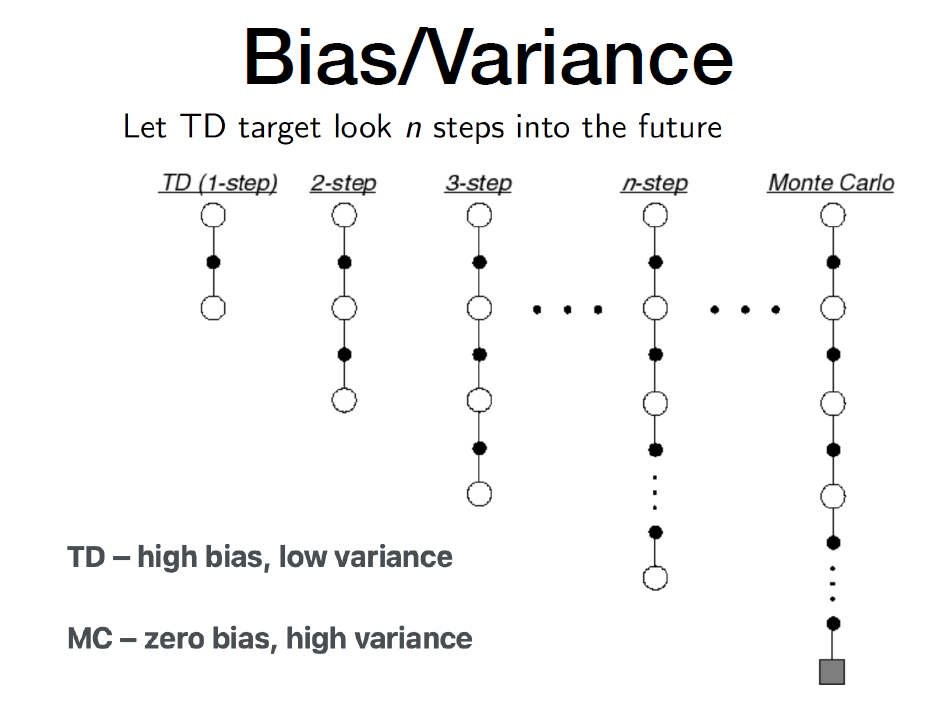
\includegraphics[keepaspectratio,alt={image.png}]{RL-DP-Algorithms_files/image.png}}
\pandocbounded{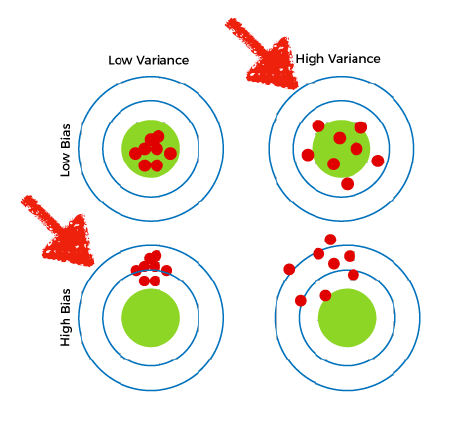
\includegraphics[keepaspectratio,alt={image-2.png}]{RL-DP-Algorithms_files/image-2.png}}

    \clearpage

✦ ✦ ✦

\subsection{Deep RL --- Value-Based}\label{deep-rl-value-based}

✦ ✦ ✦

    \phantomsection\label{dqn-naive}

    \subsubsection{DQN Naive (Deep Q-Network, no
tricks)}\label{dqn-naive-deep-q-network-no-tricks}

    \textbf{Notation:} - \(\theta\) --- neural network weights (learnable
parameters; \emph{not} a convergence threshold here) - \(Q(s,a;\theta)\)
--- Q-value approximated by a neural net with weights \(\theta\) -
\(\mathcal{L}(\theta)\) --- loss function (squared Bellman error) -
\(\nabla_\theta\) --- gradient with respect to \(\theta\)

    \phantomsection\label{intro-3-1}

    \textbf{Introduction:} Q-learning with a neural network
\(Q(s,a;\theta)\) in place of the tabular Q. \emph{Idea:} minimise the
squared one-step Bellman error
\(\mathcal{L}(\theta) = \bigl(r + \gamma \max_{a'} Q(s', a';\theta) - Q(s, a;\theta)\bigr)^2\)
via stochastic gradient descent. \emph{Why it helps:} scales Q-learning
to large/continuous state spaces (e.g.~pixel inputs) where a Q-table is
infeasible --- but this naive form is unstable because the target and
the prediction share the same rapidly changing weights \(\theta\).

    \textbf{Algorithm:}

\textbf{Input:} step size \(\alpha\), discount \(\gamma\), exploration
rate \(\varepsilon\), episodes \(n\)

\begin{enumerate}
\def\labelenumi{\arabic{enumi}.}
\item
  Initialize neural network \(Q(s,a;\theta)\) with random weights
  \(\theta\)
\item
  \textbf{For} episode \(= 1, 2, \ldots, n\) \emph{(outer loop ---
  episodes)}:

  \begin{itemize}
  \tightlist
  \item
    Initialize \(s\)
  \item
    \textbf{Repeat} for each step \emph{(inner loop --- time steps)}:

    \begin{itemize}
    \tightlist
    \item
      Choose \(a\) using \(\varepsilon\)-greedy w.r.t.
      \(Q(s,\cdot;\theta)\)
    \item
      Take action \(a\), observe \(r,\; s'\)
    \item
      \textbf{Compute target} \emph{(uses the \textbf{same} network
      \(\theta\))}:
      \[y \leftarrow r + \gamma \max_{a'} Q(s', a';\, \theta)\]
    \item
      \textbf{Gradient update:}
      \[\mathcal{L}(\theta) = \bigl(y - Q(s,a;\theta)\bigr)^2, \qquad \theta \leftarrow \theta - \alpha\,\nabla_\theta\,\mathcal{L}(\theta)\]
    \item
      \(s \leftarrow s'\)
    \end{itemize}
  \item
    Until \(s\) is terminal
  \end{itemize}
\item
  Return \(Q(\cdot,\cdot;\theta)\); derive
  \(\pi(s) = \arg\max_a Q(s,a;\theta)\)
\end{enumerate}

✦ ✦ ✦

\textbf{Problems with Naive DQN:}

\begin{itemize}
\tightlist
\item
  \textbf{Instability:} the target \(y\) depends on the same \(\theta\)
  being updated --- every gradient step shifts both the prediction and
  the target \(\Rightarrow\) \emph{moving target problem}.
\item
  \textbf{Correlated samples:} consecutive transitions \((s,a,r,s')\)
  are highly correlated; SGD assumes i.i.d. samples \(\Rightarrow\) this
  assumption is violated.
\item
  These two issues cause divergence or oscillation in practice.
\end{itemize}

\(\Rightarrow\) Fixed by \textbf{Target Network} and \textbf{Experience
Replay} (see below).

    \phantomsection\label{tricks-3-1}

    \textbf{Additional Known Engineering Tricks}

\begin{itemize}
\item
  \phantomsection\label{trick-3-1-1}\textbf{Reward clipping to
  \([-1, +1]\)} \emph{(Mnih et al., 2013)} --- clip the per-step reward
  into a fixed range before the TD target is computed. \emph{Why it
  helps:} puts all Atari games (or other tasks with wildly different
  reward magnitudes) on a single learning-rate scale; prevents a single
  jackpot reward from blowing up the gradient. \emph{Interaction:}
  changes the \emph{value of \(\gamma\) effectively} (since rewards are
  bounded), so combine with the standard \(\gamma=0.99\).
\item
  \phantomsection\label{trick-3-1-2}\textbf{Frame skipping / action
  repeat} --- repeat the same action for \(k=4\) environment steps and
  only call the network on every \(k\)-th frame. \emph{Why it helps:}
  cuts the inference cost by \(k\) and increases the effective discount
  horizon at no quality cost in environments with high temporal
  correlation between successive frames.
\item
  \phantomsection\label{trick-3-1-3}\textbf{Frame stacking} ---
  concatenate the last \(k=4\) pre-processed frames into a single
  \(k\)-channel observation. \emph{Why it helps:} injects a velocity
  signal into an otherwise-Markovian-in-pixels state; the Q-network can
  then infer motion without recurrence. \emph{Interaction:} combines
  tightly with frame skipping --- the stack contains \(k\) skipped
  frames, giving a \(k^2\)-frame temporal window.
\item
  \phantomsection\label{trick-3-1-4}\textbf{Atari pre-processing
  pipeline} --- grayscale, resize to \(84\times 84\), and take the
  \emph{pixel-wise max} over two adjacent raw frames to handle Atari's
  odd--even sprite flickering. \emph{Why it helps:} drops input
  dimensionality by \(\sim 30\times\) and removes sprite-flicker noise
  that would otherwise look like a non-Markovian observation.
\item
  \phantomsection\label{trick-3-1-5}\textbf{Huber loss (smooth L1)}
  instead of MSE --- quadratic for \(|y - Q|\le 1\), linear beyond.
  \emph{Why it helps:} equivalent to clipping the TD error gradient at
  \(\pm 1\) --- bounds the magnitude of a single bad target so a noisy
  \(y\) cannot blow up the parameters of the value head.
\item
  \phantomsection\label{trick-3-1-6}\textbf{RMSProp with low learning
  rate} \emph{(Mnih et al., 2013 --- \(\alpha=2.5\!\times\!10^{-4}\),
  momentum \(0.95\), \(\epsilon=10^{-2}\))} --- explicit per-parameter
  step normalisation. \emph{Why it helps:} compensates for
  highly-variable gradient scales across the conv stack; the specific
  small-\(\alpha\) + large-\(\epsilon\) combo is what made the
  \emph{naive} (no target net, no replay) DQN converge at all on simple
  Atari games. \emph{Interaction:} once target net + replay are added
  (next sections), Adam with \(\alpha\!\sim\!10^{-4}\) works fine and
  supersedes this choice.
\end{itemize}

    \phantomsection\label{pseudo-3-1}

    Algorithm 3.1 DQN (naive --- no target net, no replay) --- Raw
Pseudocode (without additional tricks) {[}Mnih et al., 2013{]}

Here is the pseudocode for the DQN (naive) core (base) algorithm without
any further additions and engineering tricks (also mentioned above)
added:

\textbf{Input:} step size \(\alpha\), discount \(\gamma\), exploration
rate \(\varepsilon\), episodes \(n\)\\
Initialize \(Q\)-network \(Q(s, a;\, \theta)\) with random weights
\(\theta\)\\
\textbf{for} \(\text{episode} = 1, 2, \ldots, n\) \textbf{do}\\
 Initialize \(s\)\\
 \textbf{repeat} (for each step of episode)\\
  Choose \(a\) from \(s\) using \(\varepsilon\)-greedy w.r.t.
\(Q(s, \cdot;\, \theta)\)\\
  Take action \(a\); observe \(r,\; s'\)\\
  \(y \leftarrow r + \gamma\, \max_{a'} Q(s', a';\, \theta)\)
\emph{(bootstrap from same network)}\\
  \(\mathcal{L}(\theta) \leftarrow \bigl(\, y - Q(s, a;\, \theta) \,\bigr)^{2}\)\\
  \(\theta \leftarrow \theta - \alpha\, \nabla_{\theta}\, \mathcal{L}(\theta)\)\\
  \(s \leftarrow s'\)\\
 \textbf{until} \(s\) is terminal\\
\textbf{end for}

    Algorithm 3.1 DQN (naive --- no target net, no replay) --- Pseudocode
with Additions (Engineering Tricks) {[}Mnih et al., 2013{]}

Here is the pseudocode for the DQN (naive) algorithm with also employing
all of the additions and engineering tricks mentioned above:

\textbf{Input:} ✦ RMSProp with \(\alpha\!=\!2.5\!\times\!10^{-4}\),
momentum \(0.95\), \(\epsilon_\text{opt}\!=\!10^{-2}\) ✦
(\hyperref[trick-3-1-6]{RMSProp with low learning rate}), discount
\(\gamma\), exploration \(\varepsilon\), episodes \(n\), ✦ action repeat
\(k\!=\!4\) ✦ (\hyperref[trick-3-1-2]{Frame skipping / action repeat})\\
Initialise \(Q\)-network \(Q(s, a;\, \theta)\) with random weights
\(\theta\)\\
\textbf{for} \(\text{episode} = 1, 2, \ldots, n\) \textbf{do}\\
 Initialise \(s\)\\
 ✦ Pre-process \(s\): grayscale, resize to \(84\!\times\!84\), pixel-max
over last 2 raw frames ✦ (\hyperref[trick-3-1-4]{Atari pre-processing
pipeline})\\
 ✦ Stack last \(k\!=\!4\) pre-processed frames as channels ✦
(\hyperref[trick-3-1-3]{Frame stacking})\\
 \textbf{repeat} (for each step of episode)\\
  Choose \(a\) from \(s\) using \(\varepsilon\)-greedy w.r.t.
\(Q(s, \cdot;\, \theta)\)\\
  ✦ Repeat action \(a\) for \(k\!=\!4\) environment steps; accumulate
reward ✦ (\hyperref[trick-3-1-2]{Frame skipping / action repeat})\\
  Take action \(a\); observe \(r,\; s'\)\\
  ✦ \(r \leftarrow \mathrm{clip}(r,\, -1,\, +1)\) ✦
(\hyperref[trick-3-1-1]{Reward clipping to \([-1,+1]\)})\\
  ✦ Pre-process and frame-stack \(s'\) ✦ (\hyperref[trick-3-1-4]{Atari
pre-processing pipeline} / \hyperref[trick-3-1-3]{Frame stacking})\\
  \(y \leftarrow r + \gamma\, \max_{a'} Q(s', a';\, \theta)\)\\
  ✦
\(\mathcal{L}(\theta) \leftarrow \mathrm{Huber}\bigl(y - Q(s, a;\, \theta)\bigr)\)
\emph{(smooth L1 --- linear for \(|e|>1\), quadratic otherwise)} ✦
(\hyperref[trick-3-1-5]{Huber loss (smooth L1)})\\
  ✦
\(\theta \leftarrow \theta - \mathrm{RMSProp}(\nabla_\theta\, \mathcal{L})\)
✦ (\hyperref[trick-3-1-6]{RMSProp with low learning rate})\\
  \(s \leftarrow s'\)\\
 \textbf{until} \(s\) is terminal\\
\textbf{end for}

    ✦✦✦✦✦✦✦✦✦✦✦✦✦✦✦✦✦✦✦✦✦✦✦✦✦✦✦✦✦✦✦✦✦✦✦✦✦✦✦✦✦✦✦✦✦✦✦✦✦✦

    \clearpage

\phantomsection\label{dqn-target-network}

    \subsubsection{DQN + Target Network
(DQN+TN)}\label{dqn-target-network-dqntn}

    \textbf{Notation:} - \(\theta^-\) --- frozen target network weights (a
periodic hard copy of \(\theta\); never updated by gradients) -
\(\hat{Q}(s,a;\theta^-)\) --- target network (separate from the online
network \(Q\)) - \(C\) --- target update frequency (gradient steps
between hard copies \(\theta^- \leftarrow \theta\)) - \(t\) --- global
step counter

    \phantomsection\label{intro-3-2}

    \textbf{Introduction:} DQN with a \textbf{\emph{separate frozen target
network}} \(\hat{Q}(s,a;\theta^-)\) used to compute the Bellman target;
\(\theta^-\) is a periodic hard copy of the online weights \(\theta\).
\emph{Idea:} compute the target with \(\theta^-\) instead of \(\theta\)
so the target stays still while the online network chases it, then sync
\(\theta^- \leftarrow \theta\) every \(C\) steps. \emph{Why it helps:}
fixes the moving-target problem that destabilises naive DQN ---
divergence/oscillation are replaced by a steady (if slightly stale)
regression target.

    \textbf{Algorithm:}

\textbf{Input:} \(\alpha\), \(\gamma\), \(\varepsilon\), episodes \(n\),
target update frequency \(C\)

\begin{enumerate}
\def\labelenumi{\arabic{enumi}.}
\item
  Initialize \textbf{online network} \(Q(s,a;\theta)\) with random
  weights \(\theta\)

  Initialize \textbf{target network} \(\hat{Q}(s,a;\theta^-)\) with
  \(\theta^- \leftarrow \theta\) \emph{(copy of online network)}

  Initialize step counter \(t \leftarrow 0\)
\item
  \textbf{For} episode \(= 1, 2, \ldots, n\) \emph{(outer loop ---
  episodes)}:

  \begin{itemize}
  \tightlist
  \item
    Initialize \(s\)
  \item
    \textbf{Repeat} for each step \emph{(inner loop --- time steps)}:

    \begin{itemize}
    \tightlist
    \item
      Choose \(a\) using \(\varepsilon\)-greedy w.r.t.
      \(Q(s,\cdot;\theta)\)
    \item
      Take action \(a\), observe \(r,\; s'\)
    \item
      \textbf{Compute target using frozen target network}
      \emph{(\(\theta^-\) is NOT updated here)}:
      \[y \leftarrow r + \gamma \max_{a'} \hat{Q}(s', a';\, \theta^-)\]
    \item
      \textbf{Update online network:}
      \[\mathcal{L}(\theta) = \bigl(y - Q(s,a;\theta)\bigr)^2, \qquad \theta \leftarrow \theta - \alpha\,\nabla_\theta\,\mathcal{L}(\theta)\]
    \item
      \(t \leftarrow t + 1\); if \(\;t \bmod C = 0\):
      \(\;\theta^- \leftarrow \theta\) \emph{(hard copy every \(C\)
      steps)}
    \item
      \(s \leftarrow s'\)
    \end{itemize}
  \item
    Until \(s\) is terminal
  \end{itemize}
\item
  Return \(Q(\cdot,\cdot;\theta)\); derive
  \(\pi(s) = \arg\max_a Q(s,a;\theta)\)
\end{enumerate}

✦ ✦ ✦

\textbf{Notes:}

\begin{itemize}
\tightlist
\item
  \(\theta^-\) is \textbf{frozen} between updates \(\Rightarrow\) target
  \(y\) does not shift with every gradient step \(\Rightarrow\)
  stabilizes learning.
\item
  Alternative: \textbf{soft update}
  \(\theta^- \leftarrow \tau\theta + (1-\tau)\theta^-\) with small
  \(\tau\) (e.g., \(\tau = 0.005\)) every step.
\item
  This alone still suffers from correlated samples \(\Rightarrow\)
  combine with Experience Replay.
\end{itemize}

    \phantomsection\label{tricks-3-2}

    \textbf{Additional Known Engineering Tricks}

\begin{itemize}
\item
  \phantomsection\label{trick-3-2-1}\textbf{Polyak (soft) target update}
  --- \(\theta^-\leftarrow \tau\theta + (1-\tau)\theta^-\) every step
  with small \(\tau\) (e.g., \(0.005\)). \emph{Why it helps:} smoothly
  tracks the online network with controlled lag instead of taking a
  sudden jump every \(C\) steps; the effective time constant is
  \(1/\tau\approx 200\). \emph{Interaction:} mathematically interpolates
  between hard-sync (\(\tau=1\) every step) and frozen target
  (\(\tau=0\)); pick one of hard/soft, not both. Mandatory in DDPG/SAC
  where the actor's gradient flows through the target critic and sudden
  jumps would destabilise the actor.
\item
  \phantomsection\label{trick-3-2-2}\textbf{Target network \emph{only}
  for \(\max_{a'} Q\), not for action selection at \(s\)} --- keep
  \(a\sim\varepsilon\text{-greedy}(Q(s,\cdot;\theta))\) from the
  \emph{online} net. \emph{Why it helps:} using \(\theta^-\) for
  behaviour too would make exploration stale by \(C\) steps; using
  \(\theta\) for behaviour and \(\theta^-\) only inside the regression
  target gives both fresh exploration and a stable regression problem.
\item
  \phantomsection\label{trick-3-2-3}\textbf{Asymmetric \(C\) scheduling}
  --- start with small \(C\) (≈100) during the noisy early phase and
  increase to large \(C\) later. \emph{Why it helps:} early on, the
  network is changing fast and a tight \(C\) tracks reality; later,
  learning is finer and benefits from longer-frozen targets to reduce
  target jitter.
\item
  \phantomsection\label{trick-3-2-4}\textbf{Decoupling the max}
  \emph{(precursor to Double DQN)} --- when the target network is in
  place, you have two networks lying around; use the online net to
  \emph{select} the maximising action and the target net to
  \emph{evaluate} it:
  \(y = r + \gamma\,\hat{Q}(s', \arg\max_{a'} Q(s',a';\theta);\theta^-)\).
  \emph{Why it helps:} same maximisation-bias fix as Double Q-learning,
  free from the existing two-network setup; ships as \textbf{Double DQN}
  in the full algorithm.
\item
  \phantomsection\label{trick-3-2-5}\textbf{Target net for \(V(s')\) in
  \(n\)-step bootstraps} --- when extending to \(n\)-step DQN, evaluate
  the bootstrap leaf \(Q(s_{t+n}, \cdot)\) with \(\theta^-\) but compute
  the running sum of rewards with no network involvement. \emph{Why it
  helps:} keeps the only network call in the target stable; the reward
  sum is data-only.
\end{itemize}

    \phantomsection\label{pseudo-3-2}

    Algorithm 3.2 DQN with target network --- Raw Pseudocode (without
additional tricks) {[}Mnih et al., 2015{]}

Here is the pseudocode for the DQN with target network core (base)
algorithm without any further additions and engineering tricks (also
mentioned above) added:

\textbf{Input:} \(\alpha\), \(\gamma\), \(\varepsilon\), episodes \(n\),
target update frequency \(C\)\\
Initialize online network \(Q(s, a;\, \theta)\)\\
Initialize target network \(\hat{Q}(s, a;\, \theta^{-})\) with
\(\theta^{-} \leftarrow \theta\)\\
Step counter \(t \leftarrow 0\)\\
\textbf{for} \(\text{episode} = 1, 2, \ldots, n\) \textbf{do}\\
 Initialize \(s\)\\
 \textbf{repeat} (for each step of episode)\\
  Choose \(a\) from \(s\) using \(\varepsilon\)-greedy w.r.t.
\(Q(s, \cdot;\, \theta)\)\\
  Take action \(a\); observe \(r,\; s'\)\\
  \(y \leftarrow r + \gamma\, \max_{a'} \hat{Q}(s', a';\, \theta^{-})\)
\emph{(target from frozen net)}\\
  \(\mathcal{L}(\theta) \leftarrow \bigl(\, y - Q(s, a;\, \theta) \,\bigr)^{2}\)\\
  \(\theta \leftarrow \theta - \alpha\, \nabla_{\theta}\, \mathcal{L}(\theta)\)\\
  \(s \leftarrow s';\quad t \leftarrow t + 1\)\\
  \textbf{if} \(t \bmod C = 0\) \textbf{then}
\(\theta^{-} \leftarrow \theta\)\\
 \textbf{until} \(s\) is terminal\\
\textbf{end for}

    Algorithm 3.2 DQN with target network --- Pseudocode with Additions
(Engineering Tricks) {[}Mnih et al., 2015{]}

Here is the pseudocode for the DQN with target network algorithm with
also employing all of the additions and engineering tricks mentioned
above:

\textbf{Input:} \(\alpha\), \(\gamma\), \(\varepsilon\), episodes \(n\),
✦ soft-update \(\tau\) ✦ (\hyperref[trick-3-2-1]{Polyak (soft) target
update}), ✦ initial \(C_0\), final \(C_\text{final}\) ✦
(\hyperref[trick-3-2-3]{Asymmetric \(C\) scheduling}), ✦ bootstrap steps
\(m\) ✦ (\hyperref[trick-3-2-5]{Target net for \(V(s')\) in \(n\)-step
bootstraps})\\
Initialise online network \(Q(s, a;\, \theta)\)\\
Initialise target network \(\hat{Q}(s, a;\, \theta^{-})\) with
\(\theta^{-} \leftarrow \theta\)\\
Step counter \(t \leftarrow 0\)\\
\textbf{for} \(\text{episode} = 1, 2, \ldots, n\) \textbf{do}\\
 Initialise \(s\)\\
 \textbf{repeat} (for each step of episode)\\
  ✦ Choose \(a\) from \(s\) using \(\varepsilon\)-greedy w.r.t.
\(Q(s, \cdot;\, \theta)\) \emph{(online net for behaviour, not target)}
✦ (\hyperref[trick-3-2-2]{Target network \emph{only} for
\(\max_{a'} Q\), not for action selection at \(s\)})\\
  Take action \(a\); observe \(r,\; s'\)\\
  ✦ \(a^* \leftarrow \arg\max_{a'} Q(s', a';\, \theta)\) \emph{(online
net selects)} ✦ (\hyperref[trick-3-2-4]{Decoupling the max})\\
  ✦ \(y \leftarrow r + \gamma\, \hat{Q}(s', a^*;\, \theta^{-})\)
\emph{(target net evaluates --- Double DQN)} ✦
(\hyperref[trick-3-2-4]{Decoupling the max})\\
  ✦ \emph{(For \(m\)-step bootstrap:
\(y \leftarrow \sum_{k=0}^{m-1}\gamma^k r_{t+k} + \gamma^m \hat{Q}(s_{t+m}, \cdot;\, \theta^{-})\))}
✦ (\hyperref[trick-3-2-5]{Target net for \(V(s')\) in \(n\)-step
bootstraps})\\
  \(\mathcal{L}(\theta) \leftarrow \bigl(\, y - Q(s, a;\, \theta) \,\bigr)^{2}\)\\
  \(\theta \leftarrow \theta - \alpha\, \nabla_{\theta}\, \mathcal{L}(\theta)\)\\
  \(s \leftarrow s';\quad t \leftarrow t + 1\)\\
  ✦ \(\theta^{-} \leftarrow \tau\,\theta + (1 - \tau)\,\theta^{-}\)
\emph{(Polyak soft update every step)} ✦ (\hyperref[trick-3-2-1]{Polyak
(soft) target update})\\
  ✦ \emph{(Alternative: hard sync every \(C\) steps, with \(C\)
increasing over training)} ✦ (\hyperref[trick-3-2-3]{Asymmetric \(C\)
scheduling})\\
 \textbf{until} \(s\) is terminal\\
\textbf{end for}

    ✦✦✦✦✦✦✦✦✦✦✦✦✦✦✦✦✦✦✦✦✦✦✦✦✦✦✦✦✦✦✦✦✦✦✦✦✦✦✦✦✦✦✦✦✦✦✦✦✦✦

    \clearpage

\phantomsection\label{dqn-experience-replay}

    \subsubsection{DQN + Experience Replay
(DQN+ER)}\label{dqn-experience-replay-dqner}

    \textbf{Notation:} - \(\mathcal{D}\) --- replay buffer storing past
transitions - \(M\) --- buffer capacity (max transitions stored; oldest
discarded when \(|\mathcal{D}| > M\)) - \(B\) --- minibatch size
(transitions sampled per gradient update) - \(\text{done}\) --- boolean
terminal flag: \(\text{true}\) iff \(s'\) is a terminal state

Same as DQN+TN above: - \(\theta^-\) --- frozen target network weights
(a periodic hard copy of \(\theta\); never updated by gradients) -
\(\hat{Q}(s,a;\theta^-)\) --- target network (separate from the online
network \(Q\)) - \(C\) --- target update frequency (gradient steps
between hard copies \(\theta^- \leftarrow \theta\)) - \(t\) --- global
step counter

    \phantomsection\label{intro-3-3}

    \textbf{Introduction:} The full DQN (Mnih et al., 2015). Adds an
\textbf{\emph{experience replay}} buffer on top of the target network:
every transition \((s,a,r,s',\text{done})\) is stored in a FIFO buffer
\(\mathcal{D}\), and minibatches are sampled uniformly at random for
each gradient update. \emph{Idea:} train on shuffled past transitions
instead of consecutive ones, and reuse each transition many times.
\emph{Why it helps:} decorrelates samples (consecutive trajectories
badly violate the i.i.d. assumption SGD relies on) and dramatically
improves sample efficiency by recycling data.

    \textbf{Algorithm:}

\textbf{Input:} \(\alpha\), \(\gamma\), \(\varepsilon\), episodes \(n\),
buffer capacity \(M\), minibatch size \(B\), target update freq \(C\)

\begin{enumerate}
\def\labelenumi{\arabic{enumi}.}
\item
  Initialize \textbf{online network} \(Q(s,a;\theta)\); \textbf{target
  network} \(\hat{Q}(s,a;\theta^-)\) with \(\theta^- \leftarrow \theta\)

  Initialize replay buffer \(\mathcal{D}\) with capacity \(M\); step
  counter \(t \leftarrow 0\)
\item
  \textbf{For} episode \(= 1, 2, \ldots, n\) \emph{(outer loop ---
  episodes)}:

  \begin{itemize}
  \tightlist
  \item
    Initialize \(s\)
  \item
    \textbf{Repeat} for each step \emph{(inner loop --- time steps)}:

    \begin{itemize}
    \tightlist
    \item
      Choose \(a\) using \(\varepsilon\)-greedy w.r.t.
      \(Q(s,\cdot;\theta)\)
    \item
      Take action \(a\), observe \(r,\; s',\; \text{done}\)
    \item
      Store \((s, a, r, s', \text{done})\) in \(\mathcal{D}\)
      \emph{(FIFO: oldest removed if \(|\mathcal{D}| > M\))}
    \item
      Sample \(B\) transitions
      \(\{(s_j, a_j, r_j, s'_j, \text{done}_j)\}\) uniformly from
      \(\mathcal{D}\)
    \item
      \textbf{Compute targets} for each \(j\) in minibatch:
      \[y_j = \begin{cases} r_j & \text{if } \text{done}_j \\ r_j + \gamma \max_{a'} \hat{Q}(s'_j, a';\, \theta^-) & \text{otherwise} \end{cases}\]
    \item
      \textbf{Gradient update:}
      \[\mathcal{L}(\theta) = \frac{1}{B}\sum_j \bigl(y_j - Q(s_j, a_j;\theta)\bigr)^2, \qquad \theta \leftarrow \theta - \alpha\,\nabla_\theta\,\mathcal{L}(\theta)\]
    \item
      \(t \leftarrow t+1\); if \(\;t \bmod C = 0\):
      \(\;\theta^- \leftarrow \theta\)
    \item
      \(s \leftarrow s'\)
    \end{itemize}
  \item
    Until \(s\) is terminal (\(\text{done} = \text{true}\))
  \end{itemize}
\item
  Return \(Q(\cdot,\cdot;\theta)\); derive
  \(\pi(s) = \arg\max_a Q(s,a;\theta)\)
\end{enumerate}

✦ ✦ ✦

\textbf{Notes:}

\begin{itemize}
\tightlist
\item
  \textbf{Experience Replay} breaks temporal correlation: the minibatch
  contains transitions from different episodes and time steps
  \(\Rightarrow\) approximately i.i.d. samples for SGD.
\item
  Each transition can be reused many times \(\Rightarrow\) better sample
  efficiency.
\item
  \(\mathcal{D}\) is a fixed-size FIFO queue (e.g., \(M = 10^6\)).
\item
  \(\varepsilon\) is often annealed: start at \(1.0\) (pure exploration)
  \(\to\) decay to \(0.01\) over training.
\item
  This is the standard \textbf{full DQN} algorithm. In practice, both
  tricks are always used together.
\end{itemize}

    \phantomsection\label{tricks-3-3}

    \textbf{Additional Known Engineering Tricks}

\begin{itemize}
\item
  \phantomsection\label{trick-3-3-1}\textbf{Prioritized Experience
  Replay (PER)} \emph{(Schaul et al., 2016)} --- sample transition \(j\)
  with probability \(\propto |\delta_j|^\alpha\) (the magnitude of its
  last TD error); correct the bias with importance-sampling weights
  \(w_j = (1/(N P_j))^\beta\). \emph{Why it helps:} high-error
  transitions carry more learning signal, so prioritising them speeds up
  training \(\sim 2\times\) on Atari. \emph{Interaction:} the IS weight
  is essential --- without it the \(Q\) estimate becomes biased;
  sum-trees give \(O(\log N)\) sampling.
\item
  \phantomsection\label{trick-3-3-2}\textbf{Double DQN} \emph{(van
  Hasselt, Guez \& Silver, 2016)} --- change the target to
  \(y_j = r_j + \gamma\,\hat{Q}(s'_j, \arg\max_{a'} Q(s'_j,a';\theta);\,\theta^-)\)
  --- online net selects, target net evaluates. \emph{Why it helps:}
  removes the systematic overestimation bias of \(\max_{a'} \hat{Q}\)
  for free (no extra parameters). \emph{Interaction:} needs a target
  network already, so combines trivially with the trick from the
  previous section.
\item
  \phantomsection\label{trick-3-3-3}\textbf{Dueling network
  architecture} \emph{(Wang et al., 2016)} --- split the head into a
  state-value stream \(V(s)\) and an advantage stream \(A(s,a)\),
  combine as
  \(Q(s,a) = V(s) + (A(s,a) - \tfrac{1}{|A|}\sum_{a'} A(s,a'))\).
  \emph{Why it helps:} lets the network learn the \emph{value of being
  in a state} without committing to any particular action --- important
  when actions don't affect the immediate value (e.g., navigating an
  empty corridor).
\item
  \phantomsection\label{trick-3-3-4}\textbf{Noisy Networks for
  exploration} \emph{(Fortunato et al., 2018)} --- replace the linear
  layers in the Q-network with
  \(y = (\mu_w + \sigma_w \odot \varepsilon_w)x + (\mu_b + \sigma_b \odot \varepsilon_b)\),
  with \(\varepsilon\) resampled each forward pass. \emph{Why it helps:}
  learnable \emph{parameter} noise replaces \(\varepsilon\)-greedy;
  exploration becomes state-conditional and self-tuning.
  \emph{Interaction:} makes \(\varepsilon\)-greedy unnecessary and is
  required for Rainbow.
\item
  \phantomsection\label{trick-3-3-5}\textbf{n-step bootstrap returns in
  the buffer} --- store transitions as
  \((s_t, a_t, R^{(n)}_t, s_{t+n})\) with
  \(R^{(n)}_t=\sum_{k=0}^{n-1}\gamma^k r_{t+k+1}\). \emph{Why it helps:}
  faster reward propagation, same trade-off as \(n\)-step TD; typical
  \(n=3\) on Atari. \emph{Interaction:} technically makes the target
  \emph{slightly} off-policy when combined with \(\varepsilon\)-greedy,
  but in practice the small bias is dominated by faster convergence.
\item
  \phantomsection\label{trick-3-3-6}\textbf{Distributional RL --- C51 /
  QR-DQN / IQN} \emph{(Bellemare et al., 2017; Dabney et al., 2018a,b)}
  --- replace the scalar \(Q(s,a)\) with a \emph{distribution} over
  returns (51-bin categorical for C51; quantile regression for QR-DQN;
  implicit quantile for IQN). \emph{Why it helps:} the network learns a
  richer signal (variance, skew, multimodality of returns), which
  empirically yields large gains; the policy is still
  \(\arg\max_a \mathbb{E}[Z(s,a)]\).
\item
  \phantomsection\label{trick-3-3-7}\textbf{Rainbow} \emph{(Hessel et
  al., 2018)} --- combines all six tricks above (PER + Double + Dueling
  + Noisy + n-step + Distributional) plus the basic target net + replay.
  \emph{Why it helps:} every component fixes a different failure mode of
  naive DQN; ablation studies show they are largely complementary.
\item
  \phantomsection\label{trick-3-3-8}\textbf{Replay warm-up / minimum
  buffer fill} --- collect \(\sim\!50\text{k}\) random-policy
  transitions before any gradient update. \emph{Why it helps:} ensures
  the very first minibatches are diverse enough not to overfit on a
  near-empty buffer; standard \(|\mathcal{D}|=10^6\) FIFO with min-size
  \(\sim\!5\%\) of capacity.
\end{itemize}

    \phantomsection\label{pseudo-3-3}

    Algorithm 3.3 Deep Q-learning with experience replay (full DQN) --- Raw
Pseudocode (without additional tricks) {[}Mnih et al., 2015{]}

Here is the pseudocode for the DQN with experience replay (full DQN)
core (base) algorithm without any further additions and engineering
tricks (also mentioned above) added:

\textbf{Input:} \(\alpha\), \(\gamma\), \(\varepsilon\), episodes \(n\),
buffer capacity \(M\), minibatch size \(B\), target update freq \(C\)\\
Initialize online network \(Q(s, a;\, \theta)\); target network
\(\hat{Q}(s, a;\, \theta^{-})\) with \(\theta^{-} \leftarrow \theta\)\\
Initialize replay buffer \(\mathcal{D}\) with capacity \(M\); step
counter \(t \leftarrow 0\)\\
\textbf{for} \(\text{episode} = 1, 2, \ldots, n\) \textbf{do}\\
 Initialize \(s\)\\
 \textbf{repeat} (for each step of episode)\\
  Choose \(a\) from \(s\) using \(\varepsilon\)-greedy w.r.t.
\(Q(s, \cdot;\, \theta)\)\\
  Take action \(a\); observe \(r,\; s',\; \text{done}\)\\
  Store transition \((s, a, r, s', \text{done})\) in \(\mathcal{D}\)\\
  Sample minibatch
\(\{(s_j, a_j, r_j, s'_j, \text{done}_j)\}_{j=1}^{B} \sim \mathcal{D}\)\\
  \textbf{for each} \(j\) \textbf{do}\\
   \(y_j \leftarrow r_j + \gamma\,(1 - \text{done}_j)\, \max_{a'} \hat{Q}(s'_j, a';\, \theta^{-})\)\\
  \textbf{end for}\\
  \(\mathcal{L}(\theta) \leftarrow \dfrac{1}{B}\, \sum_{j=1}^{B} \bigl(\, y_j - Q(s_j, a_j;\, \theta) \,\bigr)^{2}\)\\
  \(\theta \leftarrow \theta - \alpha\, \nabla_{\theta}\, \mathcal{L}(\theta)\)\\
  \(s \leftarrow s';\quad t \leftarrow t + 1\)\\
  \textbf{if} \(t \bmod C = 0\) \textbf{then}
\(\theta^{-} \leftarrow \theta\)\\
 \textbf{until} \(\text{done} = \mathbf{true}\)\\
\textbf{end for}

    Algorithm 3.3 Deep Q-learning with experience replay (full DQN) ---
Pseudocode with Additions (Engineering Tricks) {[}Mnih et al., 2015{]}

Here is the pseudocode for the DQN with experience replay (full DQN)
algorithm with also employing all of the additions and engineering
tricks mentioned above:

\textbf{Input:} \(\alpha\), \(\gamma\), episodes \(n\), buffer capacity
\(M\), minibatch \(B\), target update freq \(C\), ✦ PER exponent
\(\alpha_\text{per}\), IS exponent \(\beta_\text{per}\) ✦
(\hyperref[trick-3-3-1]{Prioritized Experience Replay (PER)}), ✦
bootstrap steps \(m\) ✦ (\hyperref[trick-3-3-5]{n-step bootstrap returns
in the buffer}), ✦ warm-up steps \(W\) ✦ (\hyperref[trick-3-3-8]{Replay
warm-up / minimum buffer fill})\\
✦ Initialise \(Q\)-network with dueling architecture:
\(Q(s,a) = V(s;\theta_V) + \bigl(A(s,a;\theta_A) - \tfrac{1}{|A|}\sum_{a'}A(s,a';\theta_A)\bigr)\)
✦ (\hyperref[trick-3-3-3]{Dueling network architecture})\\
✦ Replace linear layers with noisy layers:
\(y = (\mu_w + \sigma_w \odot \varepsilon)x + (\mu_b + \sigma_b \odot \varepsilon_b)\)
✦ (\hyperref[trick-3-3-4]{Noisy Networks for exploration})\\
Initialise target \(\hat{Q}\) with \(\theta^{-} \leftarrow \theta\)\\
Initialise prioritised replay buffer \(\mathcal{D}\) with capacity \(M\)
(sum-tree)\\
Step counter \(t \leftarrow 0\)\\
✦ \textbf{for} \(t = 1, \ldots, W\) \textbf{do} collect random-policy
transitions into \(\mathcal{D}\) \textbf{end for} ✦
(\hyperref[trick-3-3-8]{Replay warm-up / minimum buffer fill})\\
\textbf{for} \(\text{episode} = 1, 2, \ldots, n\) \textbf{do}\\
 Initialise \(s\)\\
 \textbf{repeat} (for each step of episode)\\
  ✦ \(a \leftarrow \arg\max_a Q(s, a;\, \theta)\)
\emph{(\(\varepsilon\)-greedy unnecessary with noisy nets)} ✦
(\hyperref[trick-3-3-4]{Noisy Networks for exploration})\\
  Take action \(a\); observe \(r,\; s',\; \text{done}\)\\
  ✦ Store \(m\)-step transition \((s_t, a_t, R^{(m)}_t, s_{t+m})\) with
\(R^{(m)}=\sum_{k=0}^{m-1}\gamma^k r_{t+k+1}\) ✦
(\hyperref[trick-3-3-5]{n-step bootstrap returns in the buffer})\\
  ✦ Sample minibatch
\(j \sim P(j) \propto |\delta_j|^{\alpha_\text{per}}\) from
\(\mathcal{D}\); compute IS weights
\(w_j = (N\,P_j)^{-\beta_\text{per}}\) ✦
(\hyperref[trick-3-3-1]{Prioritized Experience Replay (PER)})\\
  \textbf{for each} \(j\) \textbf{do}\\
   ✦ \(a^*_j \leftarrow \arg\max_{a'} Q(s'_j, a';\, \theta)\);
\(\;y_j \leftarrow R^{(m)}_j + \gamma^m(1-\text{done}_j)\,\hat{Q}(s'_j, a^*_j;\, \theta^{-})\)
\emph{(Double DQN + \(m\)-step)} ✦ (\hyperref[trick-3-3-2]{Double DQN} /
\hyperref[trick-3-3-5]{n-step bootstrap returns in the buffer})\\
  \textbf{end for}\\
  ✦
\(\mathcal{L}(\theta) \leftarrow \frac{1}{B}\sum_j w_j\bigl(\, y_j - Q(s_j, a_j;\, \theta) \,\bigr)^{2}\)
\emph{(IS-weighted loss)} ✦ (\hyperref[trick-3-3-1]{Prioritized
Experience Replay (PER)})\\
  ✦ Update priorities \(|\delta_j|\) in \(\mathcal{D}\) ✦
(\hyperref[trick-3-3-1]{Prioritized Experience Replay (PER)})\\
  ✦ \emph{(Full Rainbow: all above + distributional C51/QR-DQN head
replacing scalar \(Q\))} ✦ (\hyperref[trick-3-3-6]{Distributional RL ---
C51 / QR-DQN / IQN} / \hyperref[trick-3-3-7]{Rainbow})\\
  \(\theta \leftarrow \theta - \alpha\, \nabla_{\theta}\, \mathcal{L}(\theta);\quad s \leftarrow s';\quad t \leftarrow t + 1\)\\
  \textbf{if} \(t \bmod C = 0\) \textbf{then}
\(\theta^{-} \leftarrow \theta\)\\
 \textbf{until} \(\text{done} = \mathbf{true}\)\\
\textbf{end for}

    ✦✦✦✦✦✦✦✦✦✦✦✦✦✦✦✦✦✦✦✦✦✦✦✦✦✦✦✦✦✦✦✦✦✦✦✦✦✦✦✦✦✦✦✦✦✦✦✦✦✦

    \clearpage

✦ ✦ ✦

\subsection{Deep RL --- Policy Gradient
Methods}\label{deep-rl-policy-gradient-methods}

✦ ✦ ✦

    \phantomsection\label{vanilla-pg-loss}

\subsubsection{What Is the Vanilla Policy Gradient
Loss?}\label{what-is-the-vanilla-policy-gradient-loss}

All policy gradient methods share a common ancestor: the \textbf{policy
gradient theorem}, which gives the gradient of the expected return
\(J(\theta) = \mathbb{E}_{\pi_\theta}[R]\) with respect to the policy
parameters:

\[\nabla_\theta J(\theta) \;=\; \mathbb{E}_{\pi_\theta}\!\left[\sum_{t=0}^{T}\nabla_\theta \log\pi_\theta(a_t \mid s_t)\;\Psi_t\right]\]

The \textbf{vanilla policy gradient loss} is the objective whose
gradient recovers this formula:

\[\boxed{\;\mathcal{L}^{\text{VPG}}(\theta) \;=\; -\,\mathbb{E}\!\left[\sum_{t}\log\pi_\theta(a_t \mid s_t)\;\Psi_t\right]\;}\]

where \(\Psi_t\) is a scalar \textbf{signal} that tells the gradient
\emph{how good} action \(a_t\) was. Different choices of \(\Psi_t\)
yield different algorithms while preserving the same loss structure:

{\def\LTcaptype{none} % do not increment counter
\begin{longtable}[]{@{}
  >{\raggedright\arraybackslash}p{(\linewidth - 2\tabcolsep) * \real{0.5000}}
  >{\raggedright\arraybackslash}p{(\linewidth - 2\tabcolsep) * \real{0.5000}}@{}}
\toprule\noalign{}
\begin{minipage}[b]{\linewidth}\raggedright
\(\Psi_t\)
\end{minipage} & \begin{minipage}[b]{\linewidth}\raggedright
Algorithm
\end{minipage} \\
\midrule\noalign{}
\endhead
\bottomrule\noalign{}
\endlastfoot
\(G_t\) (full Monte-Carlo return) & REINFORCE \\
\(G_t - b(s_t)\) (baseline-subtracted return) & REINFORCE with
baseline \\
\(\delta_t = r_t + \gamma V(s_{t+1}) - V(s_t)\) (TD error) &
Actor-Critic \\
\(A_t = Q(s_t, a_t) - V(s_t)\) (advantage) & A2C / A3C \\
\end{longtable}
}

\textbf{Intuition:} increase the log-probability of actions that led to
above-average outcomes; decrease it for below-average ones. The vanilla
loss implements this idea in its simplest form --- no surrogate
objectives, no clipping, no entropy augmentation, no importance-sampling
correction.

Methods that \textbf{depart} from this vanilla template each replace or
augment the objective in a fundamental way: PPO introduces a clipped
importance-sampling surrogate, SAC adds a maximum-entropy bonus to the
reward, DDPG bypasses stochastic log-probabilities entirely via the
deterministic policy gradient, and CQL adds a conservative regulariser
for offline learning.

    {✦ Vanilla Policy Gradient}

    \clearpage

\phantomsection\label{reinforce}

    \subsubsection{REINFORCE (Monte Carlo Policy
Gradient)}\label{reinforce-monte-carlo-policy-gradient}

    \emph{Model-free, on-policy, Monte Carlo policy gradient; learns from}
\textbf{\emph{complete}} \emph{episodes.} \emph{Instead of learning
\(Q/V\), directly parameterize and optimize the} \textbf{\emph{policy}}
\(\pi(a \mid s;\theta)\)\emph{.}

    \textbf{Notation:} - \(\theta\) --- policy network weights (\emph{not} a
convergence threshold; learnable parameters of \(\pi\)) - \(J(\theta)\)
--- performance objective: expected total discounted return under policy
\(\pi(\cdot;\theta)\) - \(G_t\) --- discounted return from step \(t\) to
episode end: \(\;G_t = \sum_{k=0}^{T-t-1}\gamma^k r_{t+k+1}\) - \(T\)
--- terminal time step of the episode - \(b(s_t)\) --- baseline (any
function of \(s_t\), e.g.~\(V(s_t)\)); subtracted to reduce gradient
variance

    \phantomsection\label{intro-4-1}

    \textbf{Introduction:} Model-free, on-policy \textbf{\emph{Monte Carlo
policy gradient}} --- directly parameterises and optimises the policy
\(\pi(a \mid s;\theta)\) rather than a value function. Learns from
\textbf{\emph{complete}} episodes. \emph{Idea:} the gradient of expected
return is
\(\nabla J(\theta) = \mathbb{E}\!\left[\sum_t G_t\, \nabla\log\pi(a_t \mid s_t;\theta)\right]\)
--- increase the log-probability of actions weighted by the return that
followed them. \emph{Why it helps:} works natively for continuous and
stochastic policies, where \(\max_a Q\) is intractable; learns
stochastic policies in their own right. \emph{Cost:} high variance ---
typically reduced with a learned baseline (see Actor--Critic).

    \textbf{Algorithm:}

\textbf{Input:} policy network \(\pi(a \mid s;\theta)\), learning rate
\(\alpha\), discount \(\gamma\), episodes \(n\)

\begin{enumerate}
\def\labelenumi{\arabic{enumi}.}
\item
  Initialize policy network \(\pi(a \mid s;\theta)\) with random weights
  \(\theta\)
\item
  \textbf{For} episode \(= 1, 2, \ldots, n\) \emph{(outer loop ---
  episodes)}:

  \begin{itemize}
  \tightlist
  \item
    \textbf{--- Generate full episode using current \(\pi\) ---}
  \end{itemize}

  \[s_0,\, a_0,\, r_1,\; s_1,\, a_1,\, r_2,\; \ldots,\; s_{T-1},\, a_{T-1},\, r_T \quad \text{(run until terminal)}\]

  \begin{itemize}
  \item
    \textbf{--- Compute returns ---}
  \item
    For \(t = 0, 1, \ldots, T-1\):
    \[G_t = \sum_{k=0}^{T-t-1} \gamma^k\, r_{t+k+1}\]
  \item
    \textbf{--- Policy gradient update ---}
  \end{itemize}

  \[\theta \leftarrow \theta + \alpha \sum_{t=0}^{T-1} \gamma^t\, G_t\, \nabla_\theta \log \pi(a_t \mid s_t;\theta)\]
\item
  Return \(\pi(\cdot \mid \cdot;\theta)\)
\end{enumerate}

✦ ✦ ✦

\textbf{Policy gradient theorem:}

\[\nabla_\theta J(\theta) = \mathbb{E}_\pi\!\left[\sum_t \gamma^t\, G_t\, \nabla_\theta \log \pi(a_t \mid s_t;\theta)\right]\]

\textbf{Intuition:}

\begin{itemize}
\tightlist
\item
  \(G_t\) high \(\Rightarrow\) increase \(\log\pi(a_t \mid s_t;\theta)\)
  \(\Rightarrow\) make \(a_t\) \textbf{more likely}
\item
  \(G_t\) low \(\Rightarrow\) decrease \(\log\pi(a_t \mid s_t;\theta)\)
  \(\Rightarrow\) make \(a_t\) \textbf{less likely}
\end{itemize}

\textbf{Notes:}

\begin{itemize}
\tightlist
\item
  Must wait for a \textbf{complete} episode before updating (like MC)
  --- cannot learn online.
\item
  \textbf{High variance:} \(G_t\) can vary wildly across episodes
  \(\Rightarrow\) noisy gradient estimates.
\item
  Common fix --- subtract a \textbf{baseline} \(b(s_t)\) from \(G_t\)
  (reduces variance without adding bias):
  \[\theta \leftarrow \theta + \alpha \sum_t \gamma^t\,\bigl(G_t - b(s_t)\bigr)\,\nabla_\theta \log \pi(a_t \mid s_t;\theta)\]
  A common baseline is \(V(s_t)\) \(\Rightarrow\) this leads to
  \textbf{Actor-Critic} methods (see below).
\item
  Outputs a \textbf{stochastic} policy \(\pi(a \mid s;\theta)\), unlike
  Q-learning which outputs a deterministic policy.
\end{itemize}

    \phantomsection\label{tricks-4-1}

    \textbf{Additional Known Engineering Tricks}

\begin{itemize}
\item
  \phantomsection\label{trick-4-1-1}\textbf{Baseline subtraction} ---
  replace \(G_t\) in the gradient with \(G_t - b(s_t)\) where \(b\) is
  any function of state (commonly \(b(s)=V(s)\) from a learned critic).
  \emph{Why it helps:} \(\mathbb{E}_a[b(s)\nabla\log\pi(a\mid s)] = 0\),
  so subtracting a baseline reduces variance \emph{without adding bias}
  --- by far the most impactful single trick for REINFORCE.
  \emph{Interaction:} learning \(b=V\) alongside \(\pi\) gives
  Actor-Critic --- see Algorithm 4.2.
\item
  \phantomsection\label{trick-4-1-2}\textbf{Return standardisation
  (whitening)} --- within each episode (or batch of episodes), shift and
  scale: \(G_t \leftarrow (G_t - \mu_G) / (\sigma_G + 10^{-8})\).
  \emph{Why it helps:} removes the dependence on absolute reward scale
  and stabilises the gradient magnitude for Adam/SGD; the learning rate
  becomes scale-invariant. \emph{Interaction:} using \emph{both}
  whitening and a learned baseline subtracts the mean twice --- usually
  pick one; whitening is the cheap drop-in if no critic is trained.
\item
  \phantomsection\label{trick-4-1-3}\textbf{Adam with low learning rate
  (\(10^{-4}\,\text{–}\,10^{-3}\))} --- REINFORCE's gradient variance is
  enormous, so a small adaptive step size is essential. \emph{Why it
  helps:} Adam's per-parameter normalisation hides much of the gradient
  variance from the optimiser, allowing the small effective step to
  still make progress.
\item
  \phantomsection\label{trick-4-1-4}\textbf{Global-norm gradient
  clipping} --- if \(\|\nabla\theta\| > c\), scale to norm \(c\)
  (typical \(c\in[0.5, 5]\)). \emph{Why it helps:} a single high-return
  outlier episode can blow up the gradient; clipping caps the damage one
  bad batch can do.
\end{itemize}

    \phantomsection\label{pseudo-4-1}

    Algorithm 4.1 REINFORCE (Monte Carlo policy gradient) --- Raw Pseudocode
(without additional tricks) {[}Williams, 1992; Sutton \& Barto, §13.3{]}

Here is the pseudocode for the REINFORCE core (base) algorithm without
any further additions and engineering tricks (also mentioned above)
added:

\textbf{Input:} policy network \(\pi(a \mid s;\, \theta)\), learning
rate \(\alpha\), discount \(\gamma\), episodes \(n\)\\
Initialize \(\theta\) randomly\\
\textbf{for} \(\text{episode} = 1, 2, \ldots, n\) \textbf{do}\\
 Generate an episode using \(\pi_\theta\):
\(\;s_0, a_0, r_1,\, s_1, a_1, r_2,\, \ldots,\, s_{T-1}, a_{T-1}, r_T\)\\
 \textbf{for} \(t = 0, 1, \ldots, T - 1\) \textbf{do}\\
  \(G_t \leftarrow \displaystyle\sum_{k = t + 1}^{T} \gamma^{\,k - t - 1}\, r_k\)\\
  \(\theta \leftarrow \theta + \alpha\, \gamma^{\,t}\, G_t\, \nabla_{\theta} \log \pi(a_t \mid s_t;\, \theta)\)\\
 \textbf{end for}\\
\textbf{end for}

    Algorithm 4.1 REINFORCE (Monte Carlo policy gradient) --- Pseudocode
with Additions (Engineering Tricks) {[}Williams, 1992; Sutton \& Barto,
§13.3{]}

Here is the pseudocode for the REINFORCE algorithm with also employing
all of the additions and engineering tricks mentioned above:

\textbf{Input:} policy network \(\pi(a \mid s;\, \theta)\), ✦ Adam
optimiser with \(\alpha \in [10^{-4},\, 10^{-3}]\) ✦
(\hyperref[trick-4-1-3]{Adam with low learning rate
(\(10^{-4}\,\text{–}\,10^{-3}\))}), discount \(\gamma\), episodes \(n\),
✦ gradient clip norm \(c\) ✦ (\hyperref[trick-4-1-4]{Global-norm
gradient clipping})\\
Initialise \(\theta\) randomly\\
✦ \emph{(Optionally initialise a baseline \(b(s)\) --- e.g., a learned
\(V(s;w)\))} ✦ (\hyperref[trick-4-1-1]{Baseline subtraction})\\
\textbf{for} \(\text{episode} = 1, 2, \ldots, n\) \textbf{do}\\
 Generate an episode using \(\pi_\theta\):
\(\;s_0, a_0, r_1,\, s_1, a_1, r_2,\, \ldots,\, s_{T-1}, a_{T-1}, r_T\)\\
 \textbf{for} \(t = 0, 1, \ldots, T - 1\) \textbf{do}\\
  \(G_t \leftarrow \displaystyle\sum_{k = t + 1}^{T} \gamma^{\,k - t - 1}\, r_k\)\\
 \textbf{end for}\\
 ✦ Standardise returns:
\(G_t \leftarrow (G_t - \mu_G)/(\sigma_G + 10^{-8})\) over
\(\{G_0, \ldots, G_{T-1}\}\) ✦ (\hyperref[trick-4-1-2]{Return
standardisation (whitening)})\\
 \textbf{for} \(t = 0, 1, \ldots, T - 1\) \textbf{do}\\
  ✦
\(\theta \leftarrow \theta + \alpha\, \gamma^{\,t}\,(G_t - b(s_t))\, \nabla_{\theta} \log \pi(a_t \mid s_t;\, \theta)\)
\emph{(baseline-subtracted gradient)} ✦ (\hyperref[trick-4-1-1]{Baseline
subtraction})\\
 \textbf{end for}\\
 ✦ \textbf{if} \(\lVert\nabla\theta\rVert > c\) \textbf{then}
\(\nabla\theta \leftarrow c \cdot \nabla\theta / \lVert\nabla\theta\rVert\)
✦ (\hyperref[trick-4-1-4]{Global-norm gradient clipping})\\
 ✦ Apply Adam step ✦ (\hyperref[trick-4-1-3]{Adam with low learning rate
(\(10^{-4}\,\text{–}\,10^{-3}\))})\\
\textbf{end for}

    ✦✦✦✦✦✦✦✦✦✦✦✦✦✦✦✦✦✦✦✦✦✦✦✦✦✦✦✦✦✦✦✦✦✦✦✦✦✦✦✦✦✦✦✦✦✦✦✦✦✦

    \clearpage

\phantomsection\label{actor-critic}

    \subsubsection{Actor-Critic (AC)}\label{actor-critic-ac}

    \textbf{Notation:} - \(w\) --- critic (value network) weights -
\(\alpha_\theta\) --- actor learning rate - \(\alpha_w\) --- critic
learning rate - \(G_t\) --- discounted return from step \(t\) (same as
REINFORCE) - \(\gamma^t\) --- discounting applied to the policy gradient
at time \(t\)

    \phantomsection\label{intro-4-2}

    \textbf{Introduction:} Combines a policy gradient
(\textbf{\emph{Actor}}, \(\pi(a\mid s;\theta)\)) with a learned value
function (\textbf{\emph{Critic}}, \(V(s;w)\)). The Critic's TD error
\(\delta = r + \gamma V(s';w) - V(s;w)\) replaces the Monte Carlo return
\(G_t\) as the policy-gradient signal.

\begin{itemize}
\tightlist
\item
  \textbf{Actor:} policy network \(\pi(a \mid s;\theta)\) --- decides
  which action to take
\item
  \textbf{Critic:} value network \(V(s;w)\) --- evaluates how good the
  current state is
\end{itemize}

\emph{Idea:} let the Actor choose actions and the Critic score the
resulting states; use the Critic's verdict to push the Actor's
log-probabilities. \emph{Why it helps over REINFORCE:} much lower
variance (TD error / advantage instead of full return), and updates can
happen \textbf{\emph{online}} at every step --- no need to wait for
episode termination.

    \textbf{Algorithm:}

\textbf{Input:} actor rate \(\alpha_\theta\), critic rate \(\alpha_w\),
discount \(\gamma\), episodes \(n\)

\begin{enumerate}
\def\labelenumi{\arabic{enumi}.}
\item
  Initialize Actor \(\pi(a \mid s;\theta)\) and Critic \(V(s;w)\) with
  random weights
\item
  \textbf{For} episode \(= 1, 2, \ldots, n\) \emph{(outer loop ---
  episodes)}:

  \begin{itemize}
  \tightlist
  \item
    Initialize \(s\)
  \item
    \textbf{Repeat} for each step \emph{(inner loop --- time steps)}:

    \begin{itemize}
    \tightlist
    \item
      \(a \sim \pi(\cdot \mid s;\theta)\) \emph{(Actor chooses action)}
    \item
      Take action \(a\), observe \(r,\; s'\)
    \item
      \textbf{TD error (Critic's evaluation):}
      \[\delta \leftarrow r + \gamma V(s';w) - V(s;w)\]
      \emph{(\(\delta > 0\): outcome was better than expected;
      \(\;\delta < 0\): worse than expected)}
    \item
      \textbf{Update Critic} \emph{(minimize TD error)}:
      \[w \leftarrow w + \alpha_w\, \delta\, \nabla_w V(s;w)\]
    \item
      \textbf{Update Actor} \emph{(policy gradient with \(\delta\) as
      advantage)}:
      \[\theta \leftarrow \theta + \alpha_\theta\, \gamma^t\, \delta\, \nabla_\theta \log \pi(a \mid s;\theta)\]
      \emph{(\(\delta\) replaces \(G_t\) from REINFORCE)}
    \item
      \(s \leftarrow s'\)
    \end{itemize}
  \item
    Until \(s\) is terminal
  \end{itemize}
\item
  Return \(\pi(\cdot \mid \cdot;\theta)\)
\end{enumerate}

✦ ✦ ✦

\textbf{Notes:}

\begin{itemize}
\tightlist
\item
  Can update \textbf{every step} (online), not just at episode end.
\item
  The TD error \(\delta = r + \gamma V(s') - V(s)\) estimates the
  \textbf{advantage} \(A(s,a)\) = ``how much better was this action than
  what I expected from this state?''
\item
  \textbf{Lower variance} than REINFORCE (\(\delta\) is less noisy than
  \(G_t\)), but introduces \textbf{bias} (because \(V(s';w)\) is an
  approximation).
\item
  Two separate networks: Actor (\(\theta\)) and Critic (\(w\)), each
  with its own learning rate. They can optionally share lower layers for
  feature extraction.
\end{itemize}

    \phantomsection\label{tricks-4-2}

    \textbf{Additional Known Engineering Tricks}

\begin{itemize}
\item
  \phantomsection\label{trick-4-2-1}\textbf{Shared trunk + two heads}
  --- let actor and critic share the bulk of the network (conv stack for
  images, MLP body for state vectors), branching only at the last layer
  into a policy head and a value head. \emph{Why it helps:} one feature
  extractor is forced to encode information useful for both objectives,
  which acts as a regulariser; halves parameter count and forward-pass
  cost. \emph{Interaction:} if the actor and critic learning rates
  differ by orders of magnitude, the shared trunk's gradient can be
  dominated by one head --- fix with separate optimisers per head or
  per-head loss-scale weights.
\item
  \phantomsection\label{trick-4-2-2}\textbf{Target value network for the
  critic} --- keep a slow-moving copy \(V(s;w^-)\) and use
  \(\delta = r + \gamma V(s';w^-) - V(s;w)\) instead of \(V(s';w)\).
  \emph{Why it helps:} same logic as DQN+TN --- prevents the critic's
  bootstrap target from chasing its own moving estimate; particularly
  important when the actor and critic share weights, because actor
  gradients perturb the critic indirectly.
\item
  \phantomsection\label{trick-4-2-3}\textbf{\(n\)-step / multi-step
  bootstrapped returns} --- replace the one-step \(\delta\) with
  \(\delta^{(n)} = \sum_{k=0}^{n-1}\gamma^k r_{t+k+1} + \gamma^n V(s_{t+n};w) - V(s_t;w)\).
  \emph{Why it helps:} the same bias-variance dial as \(n\)-step TD, but
  inside the actor's advantage signal; recovers the full episode return
  at \(n=T\) (REINFORCE-style) and one-step TD at \(n=1\).
\item
  \phantomsection\label{trick-4-2-4}\textbf{Entropy regularisation}
  \(\beta\,H(\pi(\cdot\mid s))\) --- add a small positive bonus on
  policy entropy to the actor's objective. \emph{Why it helps:} prevents
  premature collapse of the stochastic policy onto a single action; on
  small problems the basic AC can converge to a near-deterministic
  suboptimal policy quickly without it. \emph{Interaction:} this is what
  A2C/A3C and PPO inherit as a non-negotiable component.
\item
  \phantomsection\label{trick-4-2-5}\textbf{Eligibility traces ---
  AC(\(\lambda\))} --- maintain traces \(e_\theta, e_w\) on both
  networks and update with \(\delta\) scaled by the trace. \emph{Why it
  helps:} offline-equivalent of the \(\lambda\)-return for both actor
  and critic, with \(O(1)\) amortised cost per step.
\item
  \phantomsection\label{trick-4-2-6}\textbf{Pop-Art / adaptive reward
  normalisation} \emph{(van Hasselt et al., 2016)} --- predict
  normalised values \(\tilde V\) and adapt the output layer's affine to
  preserve \(V\)'s scale as the running stats change. \emph{Why it
  helps:} lets the critic learn across tasks with wildly different
  reward scales without retuning the learning rate; the actor sees a
  stable advantage signal regardless.
\end{itemize}

    \phantomsection\label{pseudo-4-2}

    Algorithm 4.2 One-step Actor--Critic --- Raw Pseudocode (without
additional tricks) {[}Sutton \& Barto, §13.5{]}

Here is the pseudocode for the Actor--Critic core (base) algorithm
without any further additions and engineering tricks (also mentioned
above) added:

\textbf{Input:} actor lr \(\alpha_\theta\), critic lr \(\alpha_w\),
discount \(\gamma\), episodes \(n\)\\
Initialize policy parameters \(\theta\) and value parameters \(w\)
randomly\\
\textbf{for} \(\text{episode} = 1, 2, \ldots, n\) \textbf{do}\\
 Initialize \(s\)\\
 \(I \leftarrow 1\)\\
 \textbf{repeat} (for each step of episode)\\
  Sample \(a \sim \pi(\cdot \mid s;\, \theta)\)\\
  Take action \(a\); observe \(r,\; s'\)\\
  \(\delta \leftarrow r + \gamma\, V(s';\, w) - V(s;\, w)\) \emph{(TD
error / advantage)}\\
  \(w \leftarrow w + \alpha_w\, \delta\, \nabla_{w}\, V(s;\, w)\)\\
  \(\theta \leftarrow \theta + \alpha_\theta\, I\, \delta\, \nabla_{\theta} \log \pi(a \mid s;\, \theta)\)\\
  \(I \leftarrow \gamma\, I\)\\
  \(s \leftarrow s'\)\\
 \textbf{until} \(s\) is terminal\\
\textbf{end for}

    Algorithm 4.2 One-step Actor--Critic --- Pseudocode with Additions
(Engineering Tricks) {[}Sutton \& Barto, §13.5{]}

Here is the pseudocode for the Actor--Critic algorithm with also
employing all of the additions and engineering tricks mentioned above:

\textbf{Input:} actor lr \(\alpha_\theta\), critic lr \(\alpha_w\),
discount \(\gamma\), ✦ trace decay \(\lambda\) ✦
(\hyperref[trick-4-2-5]{Eligibility traces --- AC(\(\lambda\))}), ✦
entropy coefficient \(\beta\) ✦ (\hyperref[trick-4-2-4]{Entropy
regularisation}), ✦ bootstrap steps \(m\) ✦
(\hyperref[trick-4-2-3]{n-step / multi-step bootstrapped returns}),
episodes \(n\)\\
✦ Initialise shared-trunk network with actor head
\(\pi(\cdot\mid s;\theta)\) and critic head \(V(s;w)\) ✦
(\hyperref[trick-4-2-1]{Shared trunk + two heads})\\
✦ Initialise target critic \(V(s;w^-)\) with \(w^- \leftarrow w\) ✦
(\hyperref[trick-4-2-2]{Target value network for the critic})\\
✦ Initialise Pop-Art running stats \((\mu_r,\sigma_r)\) ✦
(\hyperref[trick-4-2-6]{Pop-Art / adaptive reward normalisation})\\
\textbf{for} \(\text{episode} = 1, 2, \ldots, n\) \textbf{do}\\
 Initialise \(s\); \(\;I \leftarrow 1\)\\
 ✦ \(e_\theta \leftarrow 0,\;e_w \leftarrow 0\) \emph{(eligibility
traces)} ✦ (\hyperref[trick-4-2-5]{Eligibility traces ---
AC(\(\lambda\))})\\
 \textbf{repeat} (for each step of episode)\\
  Sample \(a \sim \pi(\cdot \mid s;\, \theta)\)\\
  Take action \(a\); observe \(r,\; s'\)\\
  ✦ \(r \leftarrow (r - \mu_r)/\sigma_r\); update running stats
\emph{(Pop-Art)} ✦ (\hyperref[trick-4-2-6]{Pop-Art / adaptive reward
normalisation})\\
  ✦
\(\delta^{(m)} \leftarrow \sum_{k=0}^{m-1}\gamma^k r_{t+k+1} + \gamma^m V(s_{t+m};\, w^-) - V(s_t;\, w)\)
\emph{(\(m\)-step TD error via target critic)} ✦
(\hyperref[trick-4-2-3]{n-step / multi-step bootstrapped returns} /
\hyperref[trick-4-2-2]{Target value network for the critic})\\
  ✦ \(e_w \leftarrow \gamma\lambda\,e_w + \nabla_w V(s;w)\);
\(\;w \leftarrow w + \alpha_w\,\delta^{(m)}\,e_w\) ✦
(\hyperref[trick-4-2-5]{Eligibility traces --- AC(\(\lambda\))})\\
  ✦
\(e_\theta \leftarrow \gamma\lambda\,e_\theta + I\,\nabla_\theta\log\pi(a\mid s;\theta)\)
✦ (\hyperref[trick-4-2-5]{Eligibility traces --- AC(\(\lambda\))})\\
  ✦
\(\theta \leftarrow \theta + \alpha_\theta\,\delta^{(m)}\,e_\theta + \beta\,\nabla_\theta H\bigl(\pi(\cdot\mid s)\bigr)\)
\emph{(+ entropy bonus)} ✦ (\hyperref[trick-4-2-5]{Eligibility traces
--- AC(\(\lambda\))} / \hyperref[trick-4-2-4]{Entropy regularisation})\\
  \(I \leftarrow \gamma\, I\); \(\;s \leftarrow s'\)\\
 \textbf{until} \(s\) is terminal\\
\textbf{end for}

    ✦✦✦✦✦✦✦✦✦✦✦✦✦✦✦✦✦✦✦✦✦✦✦✦✦✦✦✦✦✦✦✦✦✦✦✦✦✦✦✦✦✦✦✦✦✦✦✦✦✦

    \clearpage

\phantomsection\label{a2c}

    \subsubsection{A2C (Advantage
Actor-Critic)}\label{a2c-advantage-actor-critic}

    \textbf{Notation:} - \(K\) --- number of parallel environment workers -
\(n\) --- rollout length (steps each worker collects before a gradient
update) - \(\beta\) --- entropy regularisation coefficient -
\(H(\pi(\cdot \mid s;\theta))\) --- policy entropy at state \(s\):
\(\;{-\sum_a \pi(a \mid s)\log\pi(a \mid s)}\); higher \(\Rightarrow\)
more uniform distribution \(\Rightarrow\) more exploration -
\(\mathrm{Adv}_i^k\) --- advantage estimate for worker \(k\) at step
\(i\): \(\;R - V(s_i^k;w)\)

Same as Actor-Critic above: - \(w\) --- critic (value network) weights -
\(\alpha_\theta\) --- actor learning rate - \(\alpha_w\) --- critic
learning rate

    \phantomsection\label{intro-4-3}

    \textbf{Introduction:} Synchronous advantage actor--critic. Runs \(K\)
parallel environment workers under a shared Actor and Critic;
\textbf{\emph{all workers finish their \(n\)-step rollouts}} before a
single combined gradient update is applied. \emph{Idea:} use the
\(n\)-step advantage \(\mathrm{Adv}_i = R_i - V(s_i;w)\) (lower variance
than the MC return, less biased than the 1-step TD) to drive the policy
gradient, and rely on parallel rollouts in different states for
decorrelation. \emph{Why it helps:} batches of decorrelated experiences
stabilise training (no replay buffer needed) and parallelism keeps GPU
utilisation high; in practice often matches A3C while being simpler and
avoiding stale-gradient issues.

    \textbf{Algorithm:}

\textbf{Input:} \(\alpha_\theta\), \(\alpha_w\), \(\gamma\), rollout
length \(n\), parallel workers \(K\), entropy coefficient \(\beta\)

\begin{enumerate}
\def\labelenumi{\arabic{enumi}.}
\item
  Initialize shared Actor \(\pi(a \mid s;\theta)\) and shared Critic
  \(V(s;w)\)

  Launch \(K\) parallel environment copies:
  \(\text{env}_1, \text{env}_2, \ldots, \text{env}_K\)
\item
  \textbf{Repeat} until convergence \emph{(outer loop --- updates)}:

  \begin{itemize}
  \item
    \textbf{--- Each worker \(k\) collects \(n\) steps in parallel
    (synchronously) ---}
  \item
    For each worker \(k = 1, \ldots, K\) and step \(i = 1, \ldots, n\):

    \begin{itemize}
    \tightlist
    \item
      \(a_i^k \sim \pi(\cdot \mid s_i^k;\theta)\); take \(a_i^k\) in
      \(\text{env}_k\), observe \(r_i^k,\; s_i^{\prime k}\)
    \end{itemize}
  \item
    \textbf{--- Compute \(n\)-step returns and advantages ---}
  \item
    For each worker \(k\):
    \[R \leftarrow \begin{cases} 0 & \text{if } s_n^k \text{ is terminal} \\ V(s_n^k;w) & \text{otherwise (bootstrap from Critic)} \end{cases}\]

    \begin{itemize}
    \tightlist
    \item
      For \(i = n{-}1, \ldots, 0\) (backwards):
      \(\quad R \leftarrow r_{i+1}^k + \gamma R\);
      \(\quad \mathrm{Adv}_i^k \leftarrow R - V(s_i^k;w)\)
    \end{itemize}
  \item
    \textbf{--- Aggregate losses across all \(K\) workers ---}
  \end{itemize}

  \[\mathcal{L}_\text{actor}(\theta) = -\frac{1}{K}\sum_k\sum_i \mathrm{Adv}_i^k \cdot \log\pi(a_i^k \mid s_i^k;\theta) \;-\; \beta\, H\!\bigl(\pi(\cdot \mid s_i^k;\theta)\bigr)\]

  \[\mathcal{L}_\text{critic}(w) = \frac{1}{K}\sum_k\sum_i \bigl(R - V(s_i^k;w)\bigr)^2\]

  \begin{itemize}
  \tightlist
  \item
    \textbf{--- Single synchronous gradient update ---}
  \end{itemize}

  \[\theta \leftarrow \theta - \alpha_\theta\,\nabla_\theta\,\mathcal{L}_\text{actor}, \qquad w \leftarrow w - \alpha_w\,\nabla_w\,\mathcal{L}_\text{critic}\]
\item
  Return \(\pi(\cdot \mid \cdot;\theta)\)
\end{enumerate}

✦ ✦ ✦

\textbf{Notes:}

\begin{itemize}
\tightlist
\item
  \textbf{Synchronous:} all \(K\) workers finish their rollouts, then
  ONE gradient update happens. Simpler and more stable than A3C. No
  stale gradients.
\item
  \textbf{Entropy bonus} \(\beta H(\pi)\) encourages exploration by
  penalizing overly deterministic policies:
  \(H(\pi(\cdot \mid s)) = -\sum_a \pi(a \mid s)\log\pi(a \mid s)\).
  Higher entropy \(\Rightarrow\) more uniform \(\Rightarrow\) more
  exploration.
\item
  \(K\) parallel envs \(\Rightarrow\) each update uses \(K \times n\)
  transitions \(\Rightarrow\) lower-variance gradient estimates.
\item
  \(n\)-step returns combine TD bootstrapping with multi-step actual
  rewards (like \(n\)-step TD).
\item
  In practice, actor and critic often share a neural network body with
  two output heads.
\end{itemize}

    \phantomsection\label{tricks-4-3}

    \textbf{Additional Known Engineering Tricks}

\begin{itemize}
\item
  \phantomsection\label{trick-4-3-1}\textbf{Generalised Advantage
  Estimation --- GAE(\(\lambda\))} \emph{(Schulman et al., 2016)} ---
  replace \(R - V(s)\) with
  \(\hat A_t = \sum_{l\geq 0}(\gamma\lambda)^l \delta_{t+l}\). \emph{Why
  it helps:} the same bias-variance dial as \(\lambda\)-returns, applied
  directly to the advantage; \(\lambda\!\in\![0.9, 0.97]\) is the
  empirical sweet spot in continuous-control benchmarks.
\item
  \phantomsection\label{trick-4-3-2}\textbf{Orthogonal weight
  initialisation, gain \(\sqrt{2}\)} \emph{(Saxe et al., 2014; ICLR-blog
  standard for PPO/A2C)} --- orthogonal init on hidden layers, gain
  \(0.01\) on the policy logits head, gain \(1.0\) on the value head.
  \emph{Why it helps:} the tiny gain on the logits keeps the initial
  policy nearly uniform (high entropy) so exploration starts broad;
  orthogonal weights preserve gradient norm across depth.
\item
  \phantomsection\label{trick-4-3-3}\textbf{Observation normalisation
  with running mean/std} --- maintain online estimates of per-feature
  \((\mu, \sigma)\) across all workers and feed \((s - \mu)/\sigma\) to
  the network. \emph{Why it helps:} removes the dependence on the raw
  observation scale; critical for MuJoCo-style proprioceptive inputs
  whose features differ by orders of magnitude.
\item
  \phantomsection\label{trick-4-3-4}\textbf{Advantage normalisation per
  batch} ---
  \(\hat A \leftarrow (\hat A - \mu_A)/(\sigma_A + 10^{-8})\). \emph{Why
  it helps:} the loss is then scale-invariant in advantage units; this
  is the \emph{single} most commonly-cited `magic' trick separating a
  working A2C/PPO from a broken one.
\item
  \phantomsection\label{trick-4-3-5}\textbf{Global-norm gradient
  clipping (typically \(0.5\))} --- clip \(\|\nabla(\theta,w)\|_2\) at a
  fixed norm before the optimiser step. \emph{Why it helps:} one
  anomalous rollout (e.g., a sudden mega-reward) cannot blow up the
  parameters in a single step.
\item
  \phantomsection\label{trick-4-3-6}\textbf{Frame stacking + frame
  skipping (Atari)} --- inherits the four-frame stack and
  action-repeat-4 pre-processing from DQN. \emph{Why it helps:} provides
  a velocity signal in pixel input and cuts per-decision compute,
  exactly as in value-based methods.
\end{itemize}

    \phantomsection\label{pseudo-4-3}

    Algorithm 4.3 A2C (synchronous advantage actor--critic) --- Raw
Pseudocode (without additional tricks) {[}Mnih et al., 2016 (synchronous
variant){]}

Here is the pseudocode for the A2C core (base) algorithm without any
further additions and engineering tricks (also mentioned above) added:

\textbf{Input:} \(\alpha_\theta\), \(\alpha_w\), \(\gamma\), rollout
length \(n\), parallel workers \(K\), entropy coefficient \(\beta\)\\
Initialize global parameters \(\theta\) and \(w\)\\
\textbf{repeat} until convergence\\
 \emph{// Each worker collects \(n\) steps with current
\(\pi_\theta\)}\\
 \textbf{for} \(k = 1, 2, \ldots, K\) in parallel \textbf{do}\\
  \textbf{for} \(i = 0, 1, \ldots, n - 1\) \textbf{do}\\
   Sample \(a_i^{k} \sim \pi(\cdot \mid s_i^{k};\, \theta)\); observe
\(r_{i+1}^{k},\, s_{i+1}^{k}\)\\
  \textbf{end for}\\
 \textbf{end for}\\
 \emph{// Compute \(n\)-step returns and advantages}\\
 \textbf{for} \(k = 1, 2, \ldots, K\) \textbf{do}\\
  \(R \leftarrow 0\) if \(s_n^{k}\) terminal else \(V(s_n^{k};\, w)\)\\
  \textbf{for} \(i = n - 1\) \textbf{down to} \(0\) \textbf{do}\\
   \(R \leftarrow r_{i+1}^{k} + \gamma\, R\)\\
   \(\hat{A}_i^{k} \leftarrow R - V(s_i^{k};\, w)\);\(\quad R_i^{k} \leftarrow R\)\\
  \textbf{end for}\\
 \textbf{end for}\\
 \emph{// Joint update over all \(K n\) samples}\\
 \(\mathcal{L}_\theta \leftarrow -\dfrac{1}{K n} \sum_{k, i} \bigl[\, \log \pi(a_i^{k} \mid s_i^{k};\, \theta)\, \hat{A}_i^{k} + \beta\, \mathcal{H}\bigl(\pi(\cdot \mid s_i^{k};\, \theta)\bigr) \,\bigr]\)\\
 \(\mathcal{L}_w \leftarrow \dfrac{1}{K n} \sum_{k, i} \bigl(\, R_i^{k} - V(s_i^{k};\, w) \,\bigr)^{2}\)\\
 \(\theta \leftarrow \theta - \alpha_\theta\, \nabla_{\theta}\, \mathcal{L}_\theta;\quad w \leftarrow w - \alpha_w\, \nabla_{w}\, \mathcal{L}_w\)\\
\textbf{end repeat}

    Algorithm 4.3 A2C (synchronous advantage actor--critic) --- Pseudocode
with Additions (Engineering Tricks) {[}Mnih et al., 2016 (synchronous
variant){]}

Here is the pseudocode for the A2C algorithm with also employing all of
the additions and engineering tricks mentioned above:

\textbf{Input:} \(\alpha_\theta\), \(\alpha_w\), \(\gamma\), rollout
length \(n\), parallel workers \(K\), entropy coefficient \(\beta\), ✦
GAE \(\lambda\) ✦ (\hyperref[trick-4-3-1]{Generalised Advantage
Estimation --- GAE(\(\lambda\))}), ✦ gradient clip norm \(c = 0.5\) ✦
(\hyperref[trick-4-3-5]{Global-norm gradient clipping (typically
\(0.5\))})\\
✦ Initialise shared Actor and Critic with orthogonal weights (gain
\(\sqrt{2}\) hidden, gain \(0.01\) policy head, gain \(1.0\) value head)
✦ (\hyperref[trick-4-3-2]{Orthogonal weight initialisation, gain
\(\sqrt{2}\)})\\
✦ Initialise running observation statistics \((\mu_s, \sigma_s)\) across
all workers ✦ (\hyperref[trick-4-3-3]{Observation normalisation with
running mean/std})\\
\textbf{repeat} until convergence\\
 \textbf{for} \(k = 1, 2, \ldots, K\) in parallel \textbf{do}\\
  \textbf{for} \(i = 0, 1, \ldots, n - 1\) \textbf{do}\\
   ✦ Pre-process: frame-stack + frame-skip (Atari) or normalise
\(s \leftarrow (s - \mu_s)/\sigma_s\) ✦ (\hyperref[trick-4-3-6]{Frame
stacking + frame skipping (Atari)} / \hyperref[trick-4-3-3]{Observation
normalisation with running mean/std})\\
   Sample \(a_i^{k} \sim \pi(\cdot \mid s_i^{k};\, \theta)\); observe
\(r_{i+1}^{k},\, s_{i+1}^{k}\)\\
  \textbf{end for}\\
 \textbf{end for}\\
 ✦ \emph{// Compute GAE advantages} ✦
(\hyperref[trick-4-3-1]{Generalised Advantage Estimation ---
GAE(\(\lambda\))})\\
 \textbf{for} \(k = 1, 2, \ldots, K\) \textbf{do}\\
  \(\delta_i^k \leftarrow r_{i+1}^k + \gamma\, V(s_{i+1}^k;\, w) - V(s_i^k;\, w)\)\\
  ✦
\(\hat{A}_i^{k} \leftarrow \sum_{l \geq 0}(\gamma\lambda)^l\, \delta_{i+l}^k\)
✦ (\hyperref[trick-4-3-1]{Generalised Advantage Estimation ---
GAE(\(\lambda\))})\\
  \(R_i^{k} \leftarrow \hat{A}_i^{k} + V(s_i^{k};\, w)\)\\
 \textbf{end for}\\
 ✦
\(\hat{A} \leftarrow (\hat{A} - \mu_{\hat{A}})/(\sigma_{\hat{A}} + 10^{-8})\)
✦ (\hyperref[trick-4-3-4]{Advantage normalisation per batch})\\
 \(\mathcal{L}_\theta \leftarrow -\dfrac{1}{K n} \sum_{k, i} \bigl[\, \log \pi(a_i^{k} \mid s_i^{k};\, \theta)\, \hat{A}_i^{k} + \beta\, \mathcal{H}\bigl(\pi(\cdot \mid s_i^{k};\, \theta)\bigr) \,\bigr]\)\\
 \(\mathcal{L}_w \leftarrow \dfrac{1}{K n} \sum_{k, i} \bigl(\, R_i^{k} - V(s_i^{k};\, w) \,\bigr)^{2}\)\\
 ✦ \textbf{if} \(\lVert\nabla(\theta,w)\rVert_2 > c\) \textbf{then}
rescale to norm \(c\) ✦ (\hyperref[trick-4-3-5]{Global-norm gradient
clipping (typically \(0.5\))})\\
 \(\theta \leftarrow \theta - \alpha_\theta\, \nabla_{\theta}\, \mathcal{L}_\theta;\quad w \leftarrow w - \alpha_w\, \nabla_{w}\, \mathcal{L}_w\)\\
\textbf{end repeat}

    ✦✦✦✦✦✦✦✦✦✦✦✦✦✦✦✦✦✦✦✦✦✦✦✦✦✦✦✦✦✦✦✦✦✦✦✦✦✦✦✦✦✦✦✦✦✦✦✦✦✦

    \clearpage

\phantomsection\label{a3c}

    \subsubsection{A3C (Asynchronous Advantage
Actor-Critic)}\label{a3c-asynchronous-advantage-actor-critic}

    \textbf{Notation:} - \(\theta_\text{local},\, w_\text{local}\) ---
worker-local copies of global \(\theta, w\); pulled at the start of each
rollout - \(d\theta,\, dw\) --- gradient increments computed locally and
asynchronously pushed to global params - \(K\) --- number of parallel
asynchronous workers - \(n\) --- rollout length (steps each worker
collects before pushing \(d\theta, dw\)) - \(\beta\) --- entropy
regularisation coefficient in the actor loss -
\(H(\pi(\cdot\mid s;\theta_\text{local})) = -\sum_a \pi(a\mid s;\theta_\text{local})\log\pi(a\mid s;\theta_\text{local})\)
--- policy entropy under the worker's local policy -
\(\mathrm{Adv}_i = R_i - V_{w_\text{local}}(s_i)\) --- \(n\)-step
advantage at step \(i\) within a rollout, with \(R_i\) the bootstrapped
\(n\)-step return

    \phantomsection\label{intro-4-4}

    \textbf{Introduction:} Asynchronous advantage actor--critic. \(K\)
worker threads run independent environments and
\textbf{\emph{asynchronously}} push gradient updates to a shared global
\((\theta, w)\) --- each worker pushes its gradients independently
without waiting for others. \emph{Idea:} replace experience replay with
parallelism: the diversity of states across asynchronous workers
naturally decorrelates updates, and each worker uses an \(n\)-step
advantage as in A2C. \emph{Why it helps (historically):} enabled deep
policy-gradient methods on CPU-only multi-core machines pre-GPU-friendly
batching; now largely superseded by A2C (simpler, equally fast, no stale
gradients).

    \textbf{Algorithm:}

\textbf{Input:} \(\alpha_\theta\), \(\alpha_w\), \(\gamma\), rollout
length \(n\), parallel workers \(K\), entropy coefficient \(\beta\)

\begin{enumerate}
\def\labelenumi{\arabic{enumi}.}
\item
  Initialize shared (global) Actor \(\pi(a \mid s;\theta)\) and Critic
  \(V(s;w)\)
\item
  \textbf{For each worker} \(k = 1, \ldots, K\) running
  \textbf{asynchronously} in parallel:

  \begin{itemize}
  \item
    \textbf{Repeat} \emph{(worker loop)}:

    \begin{itemize}
    \item
      \textbf{Sync:} \(\theta_\text{local} \leftarrow \theta\);
      \(\quad w_\text{local} \leftarrow w\) \emph{(pull latest global
      weights)}
    \item
      \textbf{Collect} \(n\)-step rollout using
      \(\pi(\cdot;\theta_\text{local})\):

      \begin{itemize}
      \tightlist
      \item
        For \(i = 1, \ldots, n\) (or until terminal):

        \begin{itemize}
        \tightlist
        \item
          \(a_i \sim \pi(\cdot \mid s_i;\theta_\text{local})\); take
          \(a_i\), observe \(r_i,\; s'_i\)
        \end{itemize}
      \end{itemize}
    \item
      \textbf{Compute \(n\)-step returns and advantages:}
      \[R \leftarrow \begin{cases} 0 & s_n \text{ is terminal} \\ V(s_n;w_\text{local}) & \text{otherwise (bootstrap)} \end{cases}\]

      \begin{itemize}
      \tightlist
      \item
        For \(i = n{-}1, \ldots, 0\):
        \(\quad R \leftarrow r_{i+1} + \gamma R\);
        \(\quad \mathrm{Adv}_i \leftarrow R - V(s_i;w_\text{local})\)
      \end{itemize}
    \item
      \textbf{Compute local gradients:}
      \[d\theta \leftarrow \nabla_{\theta_\text{local}}\!\left[-\sum_i \mathrm{Adv}_i \cdot \log\pi(a_i \mid s_i;\theta_\text{local}) \;-\; \beta\, H\!\bigl(\pi(\cdot \mid s_i;\theta_\text{local})\bigr)\right]\]
      \[dw \leftarrow \nabla_{w_\text{local}}\!\left[\sum_i \bigl(R - V(s_i;w_\text{local})\bigr)^2\right]\]
    \item
      \textbf{Async push to global params} \emph{(no lock --- atomic
      add)}:
      \[\theta \leftarrow \theta - \alpha_\theta\, d\theta, \qquad w \leftarrow w - \alpha_w\, dw\]
    \end{itemize}
  \item
    Until global step count reaches maximum
  \end{itemize}
\item
  Return \(\pi(\cdot \mid \cdot;\theta)\)
\end{enumerate}

✦ ✦ ✦

\textbf{Key differences from A2C:}

\begin{itemize}
\tightlist
\item
  \textbf{Asynchronous:} each worker updates global params as soon as it
  finishes its rollout, \textbf{without waiting} for other workers.
  Workers run at different speeds.
\item
  Workers may compute gradients using \textbf{stale params}
  (\(\theta_\text{local}\) may be outdated by the time the gradient is
  applied to \(\theta\)).
\item
  No replay buffer needed: the diversity of experience from \(K\) async
  workers in different states naturally decorrelates updates.
\item
  In practice, \textbf{A2C (synchronous) is often preferred} ---
  simpler, equally fast on GPU, and avoids the stale gradient issue.
\end{itemize}

    \phantomsection\label{tricks-4-4}

    \textbf{Additional Known Engineering Tricks}

\begin{itemize}
\item
  \phantomsection\label{trick-4-4-1}\textbf{HOGWILD!-style lock-free
  async updates} \emph{(Recht et al., 2011; adopted by Mnih et al.,
  2016)} --- each worker thread reads \((\theta, w)\) without a lock and
  atomically adds its gradient. \emph{Why it helps:} eliminates the
  global synchronisation barrier that bottlenecks A2C, so wall-clock
  scaling is near-linear in CPU cores. \emph{Interaction:} relies on
  gradient updates being sparse / commutative-enough that occasional
  races don't destabilise --- the entire raison d'être of A3C over A2C.
\item
  \phantomsection\label{trick-4-4-2}\textbf{Worker-local optimizer state
  (RMSProp accumulators)} --- each thread keeps its own moving-average
  squared-gradient buffer, but the parameters \(\theta\) are global.
  \emph{Why it helps:} without local optimizer state, every async write
  contaminates a single global accumulator with stale gradients and the
  adaptive step size collapses.
\item
  \phantomsection\label{trick-4-4-3}\textbf{Per-worker exploration
  parameters} --- assign each thread a \emph{different} \(\varepsilon\)
  (e.g., sampled from a log-uniform distribution) or different entropy
  bonus, drawn once per worker lifetime. \emph{Why it helps:} explicit
  diversity in the data-collecting policies replaces the experience
  replay that on-policy AC cannot use; the global parameter sees
  gradients from many exploration regimes simultaneously.
\item
  \phantomsection\label{trick-4-4-4}\textbf{LSTM policy for partial
  observability} \emph{(original A3C paper)} --- replace the
  feed-forward policy head with an LSTM whose hidden state is reset at
  episode boundaries and carried within a rollout. \emph{Why it helps:}
  lets the agent remember information beyond the current frame stack;
  the recurrent state is naturally per-worker. \emph{Interaction:} the
  asynchronous setup makes recurrent training tractable because gradient
  noise is high --- you cannot afford a tiny effective batch with BPTT
  on a single worker.
\item
  \phantomsection\label{trick-4-4-5}\textbf{Atomic gradient
  accumulation} --- push gradients via atomic-add CPU instructions
  rather than locking; on GPU implementations, fall back to small-batch
  synchronous updates because GPU memory isn't truly shared lock-freely.
  \emph{Why it helps:} the CPU-friendly version of HOGWILD! that makes
  A3C a CPU-first algorithm; on GPUs the synchronous A2C variant is
  almost always preferred.
\end{itemize}

    \phantomsection\label{pseudo-4-4}

    Algorithm 4.4 A3C --- asynchronous advantage actor--critic (per
actor-learner thread) --- Raw Pseudocode (without additional tricks)
{[}Mnih et al., 2016{]}

Here is the pseudocode for the A3C core (base) algorithm without any
further additions and engineering tricks (also mentioned above) added:

\textbf{Input:} global shared parameter vectors \(\theta\) and \(\phi\);
global shared counter \(T = 0\)\\
Assume thread-specific parameter vectors \(\theta'\) and \(\phi'\)\\
Initialize thread step counter \(t \leftarrow 1\)\\
\textbf{repeat}\\
 Reset gradients: \(d\theta \leftarrow 0\) and \(d\phi \leftarrow 0\)\\
 Synchronize thread-specific parameters \(\theta' = \theta\) and
\(\phi' = \phi\)\\
 \(t_{\text{start}} \leftarrow t\)\\
 Get state \(s_t\)\\
 \textbf{repeat}\\
  Perform \(a_t\) according to policy \(\pi(a_t \mid s_t;\, \theta')\)\\
  Receive reward \(r_t\) and new state \(s_{t+1}\)\\
  \(t \leftarrow t + 1\)\\
  \(T \leftarrow T + 1\)\\
 \textbf{until} terminal \(s_t\) \textbf{or}
\(t - t_{\text{start}} = t_{\max}\)\\
 \(R \leftarrow \begin{cases} 0 & \text{for terminal } s_t \\ V(s_t,\, \phi') & \text{for non-terminal } s_t \end{cases}\)
\emph{(bootstrap from last state)}\\
 \textbf{for} \(i \in \{t - 1, \ldots, t_{\text{start}}\}\)
\textbf{do}\\
  \(R \leftarrow r_i + \gamma\, R\)\\
  Accumulate gradients wrt \(\theta'\):
\(\;d\theta \leftarrow d\theta + \nabla_{\theta'} \log \pi(a_i \mid s_i;\, \theta')\,\bigl(R - V(s_i;\, \phi')\bigr)\)\\
  Accumulate gradients wrt \(\phi'\):
\(\;d\phi \leftarrow d\phi + \partial\bigl(R - V(s_i;\, \phi')\bigr)^{2} / \partial \phi'\)\\
 \textbf{end for}\\
 Perform asynchronous update of \(\theta\) using \(d\theta\) and of
\(\phi\) using \(d\phi\) ~HOGWILD!-style lock-free async update\\
\textbf{until} \(T > T_{\max}\)

    Algorithm 4.4 A3C --- asynchronous advantage actor--critic (per
actor-learner thread) --- Pseudocode with Additions (Engineering Tricks)
{[}Mnih et al., 2016{]}

Here is the pseudocode for the A3C algorithm with also employing all of
the additions and engineering tricks mentioned above:

\textbf{Input:} global shared parameter vectors \(\theta\) and \(\phi\);
global shared counter \(T = 0\)\\
✦ Each worker \(k\) draws its own
\(\varepsilon_k \sim \text{LogUniform}\) (or distinct entropy bonus) ✦
(\hyperref[trick-4-4-3]{Per-worker exploration parameters})\\
✦ Each worker maintains local RMSProp accumulators
\((g^2_\theta, g^2_\phi)\) ✦ (\hyperref[trick-4-4-2]{Worker-local
optimizer state (RMSProp accumulators)})\\
Assume thread-specific parameter vectors \(\theta'\) and \(\phi'\)\\
Initialise thread step counter \(t \leftarrow 1\)\\
\textbf{repeat}\\
 Reset gradients: \(d\theta \leftarrow 0\) and \(d\phi \leftarrow 0\)\\
 Synchronise thread-specific parameters \(\theta' = \theta\) and
\(\phi' = \phi\)\\
 \(t_{\text{start}} \leftarrow t\)\\
 Get state \(s_t\)\\
 ✦ Reset LSTM hidden state \(h\) at episode boundaries; carry within
rollout ✦ (\hyperref[trick-4-4-4]{LSTM policy for partial
observability})\\
 \textbf{repeat}\\
  ✦ Perform \(a_t\) according to policy
\(\pi(a_t \mid s_t, h;\, \theta')\) \emph{(LSTM policy)} ✦
(\hyperref[trick-4-4-4]{LSTM policy for partial observability})\\
  Receive reward \(r_t\) and new state \(s_{t+1}\)\\
  \(t \leftarrow t + 1\)\\
  \(T \leftarrow T + 1\)\\
 \textbf{until} terminal \(s_t\) \textbf{or}
\(t - t_{\text{start}} = t_{\max}\)\\
 \(R \leftarrow \begin{cases} 0 & \text{for terminal } s_t \\ V(s_t,\, \phi') & \text{for non-terminal } s_t \end{cases}\)\\
 \textbf{for} \(i \in \{t - 1, \ldots, t_{\text{start}}\}\)
\textbf{do}\\
  \(R \leftarrow r_i + \gamma\, R\)\\
  Accumulate gradients wrt \(\theta'\):
\(\;d\theta \leftarrow d\theta + \nabla_{\theta'} \log \pi(a_i \mid s_i;\, \theta')\,\bigl(R - V(s_i;\, \phi')\bigr)\)\\
  Accumulate gradients wrt \(\phi'\):
\(\;d\phi \leftarrow d\phi + \partial\bigl(R - V(s_i;\, \phi')\bigr)^{2} / \partial \phi'\)\\
 \textbf{end for}\\
 ✦ Atomically add \(d\theta\) to global \(\theta\) and \(d\phi\) to
global \(\phi\) \emph{(lock-free HOGWILD! update via atomic CPU
instructions)} ✦ (\hyperref[trick-4-4-1]{HOGWILD!-style lock-free async
updates} / \hyperref[trick-4-4-5]{Atomic gradient accumulation})\\
 ✦ Update worker-local RMSProp accumulators ✦
(\hyperref[trick-4-4-2]{Worker-local optimizer state (RMSProp
accumulators)})\\
\textbf{until} \(T > T_{\max}\)

    ✦✦✦✦✦✦✦✦✦✦✦✦✦✦✦✦✦✦✦✦✦✦✦✦✦✦✦✦✦✦✦✦✦✦✦✦✦✦✦✦✦✦✦✦✦✦✦✦✦✦

    {✦ Advanced Policy Optimization}

    \clearpage

\phantomsection\label{ddpg}

    \subsubsection{DDPG (Deep Deterministic Policy
Gradient)}\label{ddpg-deep-deterministic-policy-gradient}

    \emph{Off-policy, actor-critic for} \textbf{\emph{continuous action
spaces}}. \emph{Combines DPG with DQN tricks (target networks +
replay).} \emph{Like DQN but the \(\max_a Q\) is replaced by the actor's
output \(\mu(s)\), since enumerating \(a\) is infeasible in
\(\mathbb{R}^d\).}

    \textbf{Notation:} - \(\mu(s;\theta^\mu)\) --- \textbf{deterministic}
actor (policy network); outputs a single continuous action vector, not a
distribution - \(Q(s,a;\theta^Q)\) --- critic (state-action value
network) - \(\theta^{\mu-},\,\theta^{Q-}\) --- target actor and target
critic weights (slow-moving copies of \(\theta^\mu, \theta^Q\)) -
\(\tau\) --- Polyak soft-update coefficient (e.g., \(\tau = 0.005\)):
\(\;\theta^- \leftarrow \tau\theta + (1-\tau)\theta^-\) -
\(\mathcal{N}_t\) --- exploration noise added to actions (e.g.,
Ornstein-Uhlenbeck or Gaussian) - \(\mathcal{D},\,B,\,M\) --- replay
buffer, minibatch size, capacity (same as DQN+ER)

    \phantomsection\label{intro-4-5}

    \textbf{Introduction:} Off-policy actor--critic for
\textbf{\emph{continuous action spaces}}. Combines the deterministic
policy gradient (DPG) with DQN-style tricks (target networks + replay
buffer). \emph{Idea:} learn a \textbf{\emph{deterministic}} actor
\(\mu(s;\theta^\mu)\) alongside a Q-critic \(Q(s,a;\theta^Q)\). Since
\(\max_a Q\) is intractable in \(\mathbb{R}^d\), replace it with
\(Q(s, \mu(s))\) and update the actor by gradient ascent on this --- the
chain rule pushes \(\mu\) toward actions that the critic rates highly.
\emph{Why it helps:} brings DQN-style off-policy learning to continuous
control, where Q-learning's \(\arg\max\) cannot be enumerated.

    \textbf{Algorithm:}

\textbf{Input:} actor rate \(\alpha_\mu\), critic rate \(\alpha_Q\),
discount \(\gamma\), soft-update \(\tau\), buffer capacity \(M\),
minibatch size \(B\), episodes \(n\)

\begin{enumerate}
\def\labelenumi{\arabic{enumi}.}
\item
  Initialize Actor \(\mu(s;\theta^\mu)\) and Critic \(Q(s,a;\theta^Q)\)
  with random weights

  Initialize target networks \(\theta^{\mu-} \leftarrow \theta^\mu\),
  \(\;\theta^{Q-} \leftarrow \theta^Q\)

  Initialize replay buffer \(\mathcal{D}\) with capacity \(M\)
\item
  \textbf{For} episode \(= 1, 2, \ldots, n\) \emph{(outer loop ---
  episodes)}:

  \begin{itemize}
  \tightlist
  \item
    Initialize \(s\) and exploration noise process \(\mathcal{N}\)
  \item
    \textbf{Repeat} for each step \emph{(inner loop --- time steps)}:

    \begin{itemize}
    \tightlist
    \item
      \(a \leftarrow \mu(s;\theta^\mu) + \mathcal{N}_t\)
      \emph{(deterministic action + exploration noise)}
    \item
      Take action \(a\), observe \(r,\; s',\; \text{done}\)
    \item
      Store \((s, a, r, s', \text{done})\) in \(\mathcal{D}\)
    \item
      Sample \(B\) transitions
      \(\{(s_j, a_j, r_j, s'_j, \text{done}_j)\}\) uniformly from
      \(\mathcal{D}\)
    \item
      \textbf{Compute critic target} \emph{(uses target actor and target
      critic)}:
      \[y_j = \begin{cases} r_j & \text{if } \text{done}_j \\ r_j + \gamma\, Q\!\bigl(s'_j,\, \mu(s'_j;\theta^{\mu-});\, \theta^{Q-}\bigr) & \text{otherwise} \end{cases}\]
    \item
      \textbf{Update Critic} \emph{(minimize squared Bellman error)}:
      \[\mathcal{L}(\theta^Q) = \frac{1}{B}\sum_j \bigl(y_j - Q(s_j, a_j;\theta^Q)\bigr)^2, \qquad \theta^Q \leftarrow \theta^Q - \alpha_Q\,\nabla_{\theta^Q}\,\mathcal{L}(\theta^Q)\]
    \item
      \textbf{Update Actor} \emph{(deterministic policy gradient ---
      chain rule through Q)}:
      \[\nabla_{\theta^\mu} J \approx \frac{1}{B}\sum_j \nabla_a Q(s_j, a;\theta^Q)\big|_{a=\mu(s_j)} \cdot \nabla_{\theta^\mu} \mu(s_j;\theta^\mu)\]
      \[\theta^\mu \leftarrow \theta^\mu + \alpha_\mu\,\nabla_{\theta^\mu} J\]
    \item
      \textbf{Soft-update target networks} \emph{(Polyak averaging)}:
      \[\theta^{Q-} \leftarrow \tau\theta^Q + (1-\tau)\theta^{Q-}, \qquad \theta^{\mu-} \leftarrow \tau\theta^\mu + (1-\tau)\theta^{\mu-}\]
    \item
      \(s \leftarrow s'\)
    \end{itemize}
  \item
    Until \(s\) is terminal
  \end{itemize}
\item
  Return \(\mu(\cdot;\theta^\mu)\)
\end{enumerate}

✦ ✦ ✦

\textbf{Notes:}

\begin{itemize}
\tightlist
\item
  \textbf{Continuous actions:} the \(\max_{a'}\) in DQN's Bellman target
  is replaced by \(Q(s', \mu(s';\theta^{\mu-}))\) --- the actor
  \emph{approximates} the argmax over continuous \(a\).
\item
  \textbf{Deterministic policy gradient} (Silver et al., 2014): for a
  deterministic \(\mu\), the policy gradient simplifies to
  \(\nabla_a Q \cdot \nabla_{\theta^\mu} \mu\) (chain rule through the
  critic).
\item
  \textbf{Exploration is external:} since \(\mu\) is deterministic,
  exploration is injected via additive noise \(\mathcal{N}_t\) on the
  action (Ornstein-Uhlenbeck for temporally correlated noise, or simple
  Gaussian).
\item
  \textbf{Soft target updates:} rather than hard copies every \(C\)
  steps (DQN), target networks slowly track the online networks:
  \(\theta^- \leftarrow \tau\theta + (1-\tau)\theta^-\).
\item
  \textbf{Known weaknesses:} brittle to hyperparameters, \textbf{critic
  Q-value overestimation} (similar to DQN max bias). Fixed by
  \textbf{TD3} (twin critics + delayed actor updates + target action
  smoothing) and \textbf{SAC} (entropy regularisation, stochastic
  policy).
\end{itemize}

    \phantomsection\label{tricks-4-5}

    \textbf{Additional Known Engineering Tricks}

\begin{itemize}
\item
  \phantomsection\label{trick-4-5-1}\textbf{Layer normalisation in
  critic and actor} --- apply LayerNorm after each hidden layer; the
  original DDPG paper used BatchNorm but it interacts badly with replay
  (running stats drift). \emph{Why it helps:} normalises feature scales,
  which is critical because state vectors in continuous control span
  very different magnitudes per dimension.
\item
  \phantomsection\label{trick-4-5-2}\textbf{Parameter-space noise for
  exploration} \emph{(Plappert et al., 2017)} --- perturb \(\theta^\mu\)
  itself with Gaussian noise (re-sampled every \(K\) steps) instead of
  adding \(\mathcal{N}_t\) to the action. \emph{Why it helps:} yields
  state-consistent exploration (the same state evokes the same perturbed
  action within a rollout), which acts as a primitive over
  time-correlated noise; combine with action-space noise via an adaptive
  scale schedule.
\item
  \phantomsection\label{trick-4-5-3}\textbf{Tanh action squashing +
  reward/state scaling} --- pass the actor output through \(\tanh\) and
  rescale to \([a_\text{low}, a_\text{high}]\); centre and unit-scale
  rewards via running stats. \emph{Why it helps:} keeps actions bounded
  without clipping (clipping kills the gradient); reward scaling means
  the same learning rate works across tasks with wildly different reward
  magnitudes.
\item
  \phantomsection\label{trick-4-5-4}\textbf{TD3 extensions}
  \emph{(Fujimoto et al., 2018)} --- three drop-in fixes for DDPG's
  instability: (i) \textbf{twin critics} with target
  \(y = r + \gamma\,\min_{i=1,2} Q_{\theta_i^-}(s', \mu(s';\theta^{\mu-}))\);
  (ii) \textbf{delayed actor \& target updates} every 2 critic steps;
  (iii) \textbf{target action smoothing}
  \(\tilde a = \mu(s';\theta^{\mu-}) + \mathrm{clip}(\epsilon, -c, c)\),
  \(\epsilon\sim\mathcal{N}(0,\sigma_t^2)\). \emph{Why each helps:}
  twin-min combats critic overestimation; delayed actor updates wait for
  the critic to catch up before changing the policy; target smoothing
  forces the critic to be smooth in the action input, killing
  exploitable sharp critic peaks. \emph{Interaction:} these are
  essentially \emph{the} fix to DDPG and are almost always applied ---
  bare DDPG is rarely used.
\item
  \phantomsection\label{trick-4-5-5}\textbf{Replay warm-up with random
  actor} --- for the first \(\sim\!10\text{k}\) steps, sample uniformly
  from the action space instead of using \(\mu(s)\). \emph{Why it
  helps:} the freshly-initialised critic has uninformative Q-values;
  sampling random actions gives diverse coverage to bootstrap learning,
  similar to DQN's \(\varepsilon\!=\!1\) warm-up.
\end{itemize}

    \phantomsection\label{pseudo-4-5}

    Algorithm 4.5 DDPG (deep deterministic policy gradient) --- Raw
Pseudocode (without additional tricks) {[}Lillicrap et al., 2016{]}

Here is the pseudocode for the DDPG core (base) algorithm without any
further additions and engineering tricks (also mentioned above) added:

\textbf{Input:} actor lr \(\alpha_\mu\), critic lr \(\alpha_Q\),
discount \(\gamma\), soft-update \(\tau\), buffer capacity \(M\),
minibatch size \(B\), episodes \(n\)\\
Initialize critic \(Q(s, a;\, \theta^{Q})\) and actor
\(\mu(s;\, \theta^{\mu})\) with random weights\\
Initialize target networks:
\(\theta^{Q'} \leftarrow \theta^{Q},\;\theta^{\mu'} \leftarrow \theta^{\mu}\)\\
Initialize replay buffer \(\mathcal{D}\) with capacity \(M\)\\
\textbf{for} \(\text{episode} = 1, 2, \ldots, n\) \textbf{do}\\
 Initialize exploration noise process \(\mathcal{N}\)\\
 Initialize \(s\)\\
 \textbf{repeat} (for each step of episode)\\
  \(a \leftarrow \mu(s;\, \theta^{\mu}) + \mathcal{N}_t\)\\
  Take action \(a\); observe \(r,\; s',\; \text{done}\)\\
  Store \((s, a, r, s', \text{done})\) in \(\mathcal{D}\)\\
  Sample minibatch
\(\{(s_j, a_j, r_j, s'_j, \text{done}_j)\}_{j=1}^{B} \sim \mathcal{D}\)\\
  \(y_j \leftarrow r_j + \gamma\,(1 - \text{done}_j)\, Q\bigl(s'_j,\, \mu(s'_j;\, \theta^{\mu'});\, \theta^{Q'}\bigr)\)\\
  \(\mathcal{L}_Q \leftarrow \dfrac{1}{B} \sum_j \bigl(\, y_j - Q(s_j, a_j;\, \theta^{Q}) \,\bigr)^{2}\)\\
  \(\theta^{Q} \leftarrow \theta^{Q} - \alpha_Q\, \nabla_{\theta^{Q}}\, \mathcal{L}_Q\)\\
  \(\nabla_{\theta^{\mu}} J \approx \dfrac{1}{B} \sum_j \nabla_a\, Q(s_j, a;\, \theta^{Q})\bigr|_{a = \mu(s_j;\, \theta^{\mu})}\, \nabla_{\theta^{\mu}}\, \mu(s_j;\, \theta^{\mu})\)\\
  \(\theta^{\mu} \leftarrow \theta^{\mu} + \alpha_\mu\, \nabla_{\theta^{\mu}} J\)\\
  \emph{// Soft target updates (Polyak averaging)}\\
  \(\theta^{Q'} \leftarrow \tau\, \theta^{Q} + (1 - \tau)\, \theta^{Q'}\)\\
  \(\theta^{\mu'} \leftarrow \tau\, \theta^{\mu} + (1 - \tau)\, \theta^{\mu'}\)\\
  \(s \leftarrow s'\)\\
 \textbf{until} \(s\) is terminal\\
\textbf{end for}

    Algorithm 4.5 DDPG (deep deterministic policy gradient) --- Pseudocode
with Additions (Engineering Tricks) {[}Lillicrap et al., 2016{]}

Here is the pseudocode for the DDPG algorithm with also employing all of
the additions and engineering tricks mentioned above:

\textbf{Input:} actor lr \(\alpha_\mu\), critic lr \(\alpha_Q\),
discount \(\gamma\), soft-update \(\tau\), buffer capacity \(M\),
minibatch size \(B\), episodes \(n\), ✦ warm-up steps
\(W\!\approx\!10\text{k}\) ✦ (\hyperref[trick-4-5-5]{Replay warm-up with
random actor}), ✦ TD3 smoothing noise \(\sigma_t\), clip \(c\) ✦
(\hyperref[trick-4-5-4]{TD3 extensions})\\
✦ Initialise twin critics \(Q_{\theta_1^Q}, Q_{\theta_2^Q}\) with
LayerNorm after each hidden layer ✦ (\hyperref[trick-4-5-1]{Layer
normalisation in critic and actor} / \hyperref[trick-4-5-4]{TD3
extensions})\\
✦ Initialise actor \(\mu(s;\,\theta^\mu)\) with LayerNorm; output
through \(\tanh\) rescaled to \([a_\text{low}, a_\text{high}]\) ✦
(\hyperref[trick-4-5-1]{Layer normalisation in critic and actor} /
\hyperref[trick-4-5-3]{Tanh action squashing + reward/state scaling})\\
Initialise targets:
\(\theta_i^{Q'} \leftarrow \theta_i^Q,\;\theta^{\mu'} \leftarrow \theta^\mu\)\\
Initialise replay buffer \(\mathcal{D}\) with capacity \(M\)\\
✦ Maintain running reward/state statistics
\((\mu_r,\sigma_r),(\mu_s,\sigma_s)\) ✦ (\hyperref[trick-4-5-3]{Tanh
action squashing + reward/state scaling})\\
✦ \textbf{for} first \(W\) steps \textbf{do} sample
\(a \sim \mathrm{Uniform}(a_\text{low}, a_\text{high})\), store in
\(\mathcal{D}\) \textbf{end for} ✦ (\hyperref[trick-4-5-5]{Replay
warm-up with random actor})\\
\textbf{for} \(\text{episode} = 1, 2, \ldots, n\) \textbf{do}\\
 Initialise \(s\)\\
 ✦ \emph{(Optionally perturb \(\theta^\mu\) with Gaussian noise for
parameter-space exploration)} ✦ (\hyperref[trick-4-5-2]{Parameter-space
noise for exploration})\\
 \textbf{repeat} (for each step of episode)\\
  ✦
\(a \leftarrow \tanh\!\bigl(\mu((s-\mu_s)/\sigma_s;\,\theta^\mu)\bigr) \cdot \text{scale} + \mathcal{N}_t\)
\emph{(or use parameter-space noise)} ✦ (\hyperref[trick-4-5-3]{Tanh
action squashing + reward/state scaling} /
\hyperref[trick-4-5-2]{Parameter-space noise for exploration})\\
  Take action \(a\); observe \(r,\; s',\; \text{done}\)\\
  ✦ \(r \leftarrow r / \sigma_r\) \emph{(reward scaling)} ✦
(\hyperref[trick-4-5-3]{Tanh action squashing + reward/state scaling})\\
  Store \((s, a, r, s', \text{done})\) in \(\mathcal{D}\)\\
  Sample minibatch
\(\{(s_j, a_j, r_j, s'_j, \text{done}_j)\}_{j=1}^{B} \sim \mathcal{D}\)\\
  ✦
\(\tilde{a}' \leftarrow \mu(s'_j;\,\theta^{\mu'}) + \mathrm{clip}(\epsilon,\, -c,\, c),\;\epsilon\sim\mathcal{N}(0,\sigma_t^2)\)
\emph{(target action smoothing)} ✦ (\hyperref[trick-4-5-4]{TD3
extensions})\\
  ✦
\(y_j \leftarrow r_j + \gamma\,(1-\text{done}_j)\,\min_{i=1,2} Q_{\theta_i^{Q'}}(s'_j, \tilde{a}')\)
\emph{(twin-min target)} ✦ (\hyperref[trick-4-5-4]{TD3 extensions})\\
  \textbf{for} \(i = 1, 2\) \textbf{do}
\(\;\theta_i^Q \leftarrow \theta_i^Q - \alpha_Q\,\nabla_{\theta_i^Q}\,\frac{1}{B}\sum_j(y_j - Q_{\theta_i^Q}(s_j,a_j))^2\)
\textbf{end for}\\
  ✦ \textbf{if} \(t \bmod 2 = 0\) \textbf{then} \emph{(delayed actor +
target updates)} ✦ (\hyperref[trick-4-5-4]{TD3 extensions})\\
   \(\nabla_{\theta^{\mu}} J \approx \dfrac{1}{B} \sum_j \nabla_a\, Q_{\theta_1^Q}(s_j, a)\bigr|_{a = \mu(s_j;\, \theta^{\mu})}\, \nabla_{\theta^{\mu}}\, \mu(s_j;\, \theta^{\mu})\)\\
   \(\theta^{\mu} \leftarrow \theta^{\mu} + \alpha_\mu\, \nabla_{\theta^{\mu}} J\)\\
   \(\theta_i^{Q'} \leftarrow \tau\, \theta_i^Q + (1 - \tau)\, \theta_i^{Q'};\quad \theta^{\mu'} \leftarrow \tau\, \theta^{\mu} + (1 - \tau)\, \theta^{\mu'}\)\\
  ✦ \textbf{end if} ✦ (\hyperref[trick-4-5-4]{TD3 extensions})\\
  \(s \leftarrow s'\)\\
 \textbf{until} \(s\) is terminal\\
\textbf{end for}

    ✦✦✦✦✦✦✦✦✦✦✦✦✦✦✦✦✦✦✦✦✦✦✦✦✦✦✦✦✦✦✦✦✦✦✦✦✦✦✦✦✦✦✦✦✦✦✦✦✦✦

    \clearpage

\phantomsection\label{sac}

    \subsubsection{SAC (Soft Actor-Critic)}\label{sac-soft-actor-critic}

    \emph{Off-policy, actor-critic for continuous actions. Builds on DDPG
with:} \textbf{\emph{stochastic policy}}, \textbf{\emph{twin critics}}
\emph{(min combats overestimation, as in TD3), and a}
\textbf{\emph{maximum-entropy objective}} \emph{that explicitly rewards
exploration.}

    \textbf{Notation:} - \(\pi(a \mid s;\phi)\) --- \textbf{stochastic}
Gaussian actor (typically \(\tanh\)-squashed): outputs
\((\mu_\phi(s), \sigma_\phi(s))\); action
\(a = \tanh(\mu_\phi(s) + \sigma_\phi(s) \odot \xi),\; \xi \sim \mathcal{N}(0, I)\)
- \(Q_{\theta_1}, Q_{\theta_2}\) --- \textbf{twin critics} (two
independent Q-networks; using the min combats overestimation) -
\(\theta_1^-,\,\theta_2^-\) --- target critic weights (Polyak soft
updates with coefficient \(\tau\)) - \(\alpha\) --- \textbf{entropy
temperature}: trades off expected return vs.~policy entropy (can be
tuned automatically toward a target entropy \(\bar{H}\)) -
\(H(\pi(\cdot \mid s)) = -\mathbb{E}_{a\sim\pi}[\log\pi(a \mid s)]\) ---
policy entropy at state \(s\) - \(\mathcal{D},\,B,\,\tau\) --- replay
buffer, minibatch size, soft-update coefficient (as in DDPG)

    \phantomsection\label{intro-4-6}

    \textbf{Introduction:} Off-policy actor--critic for continuous actions.
Builds on DDPG with three key changes: a \textbf{\emph{stochastic}}
(Gaussian, \(\tanh\)-squashed) actor, \textbf{\emph{twin critics}} that
take the min to combat overestimation (as in TD3), and a
\textbf{\emph{maximum-entropy objective}} that explicitly rewards
exploration.

\textbf{Maximum-entropy objective:}

\[J(\pi) = \mathbb{E}\!\left[\sum_t \gamma^t \bigl(r_t + \alpha\, H(\pi(\cdot \mid s_t))\bigr)\right]\]

\emph{The agent maximises reward} \textbf{\emph{plus}} \emph{expected
entropy --- staying as random as possible while still solving the task.
Why it helps:} the stochastic policy explores natively (no external
noise needed), twin critics tame the overestimation that destabilises
DDPG, and the entropy bonus prevents premature collapse to a
deterministic local optimum --- yielding state-of-the-art sample
efficiency on continuous control.

    \textbf{Algorithm:}

\textbf{Input:} actor rate \(\alpha_\phi\), critic rate \(\alpha_Q\),
discount \(\gamma\), soft-update \(\tau\), temperature \(\alpha\),
buffer capacity \(M\), minibatch size \(B\), episodes \(n\)

\begin{enumerate}
\def\labelenumi{\arabic{enumi}.}
\item
  Initialize twin critics \(Q_{\theta_1}, Q_{\theta_2}\) and stochastic
  actor \(\pi(a \mid s;\phi)\)

  Initialize target critics \(\theta_1^- \leftarrow \theta_1\),
  \(\;\theta_2^- \leftarrow \theta_2\)

  Initialize replay buffer \(\mathcal{D}\) with capacity \(M\)
\item
  \textbf{For} episode \(= 1, 2, \ldots, n\) \emph{(outer loop ---
  episodes)}:

  \begin{itemize}
  \tightlist
  \item
    Initialize \(s\)
  \item
    \textbf{Repeat} for each step \emph{(inner loop --- time steps)}:

    \begin{itemize}
    \item
      \(a \sim \pi(\cdot \mid s;\phi)\) \emph{(sample from stochastic
      policy --- exploration is built in)}
    \item
      Take action \(a\), observe \(r,\; s',\; \text{done}\); store
      \((s, a, r, s', \text{done})\) in \(\mathcal{D}\)
    \item
      Sample \(B\) transitions
      \(\{(s_j, a_j, r_j, s'_j, \text{done}_j)\}\) from \(\mathcal{D}\)
    \item
      \textbf{--- Critic targets (entropy-augmented, with twin min) ---}
    \item
      Sample \(\tilde{a}'_j \sim \pi(\cdot \mid s'_j;\phi)\) for each
      \(j\) \emph{(fresh sample from current actor)}
    \item
      \[y_j = r_j + \gamma\,(1-\text{done}_j)\Bigl[\min_{i=1,2} Q_{\theta_i^-}(s'_j, \tilde{a}'_j) \;-\; \alpha\, \log\pi(\tilde{a}'_j \mid s'_j;\phi)\Bigr]\]
    \item
      \textbf{--- Update both critics ---}

      \[\mathcal{L}(\theta_i) = \frac{1}{B}\sum_j \bigl(y_j - Q_{\theta_i}(s_j, a_j)\bigr)^2,\quad \theta_i \leftarrow \theta_i - \alpha_Q\,\nabla_{\theta_i}\,\mathcal{L}(\theta_i),\quad i=1,2\]
    \item
      \textbf{--- Update actor (reparameterised --- gradient flows
      through sample) ---}
    \item
      Sample
      \(\tilde{a}_j = \tanh(\mu_\phi(s_j) + \sigma_\phi(s_j) \odot \xi_j),\; \xi_j \sim \mathcal{N}(0,I)\)
      \[\mathcal{L}(\phi) = \frac{1}{B}\sum_j \Bigl[\alpha\,\log\pi(\tilde{a}_j \mid s_j;\phi) \;-\; \min_{i=1,2} Q_{\theta_i}(s_j, \tilde{a}_j)\Bigr]\]
      \[\phi \leftarrow \phi - \alpha_\phi\,\nabla_\phi\,\mathcal{L}(\phi)\]
    \item
      \textbf{(Optional) Auto-tune temperature} \(\alpha\) toward target
      entropy \(\bar{H}\):
      \[\mathcal{L}(\alpha) = -\alpha\,\mathbb{E}_{a\sim\pi}\bigl[\log\pi(a \mid s) + \bar{H}\bigr],\qquad \alpha \leftarrow \alpha - \alpha_\alpha\,\nabla_\alpha\,\mathcal{L}(\alpha)\]
    \item
      \textbf{Soft-update target critics:}
      \(\;\theta_i^- \leftarrow \tau\theta_i + (1-\tau)\theta_i^-,\quad i=1,2\)
    \item
      \(s \leftarrow s'\)
    \end{itemize}
  \item
    Until \(s\) is terminal
  \end{itemize}
\item
  Return \(\pi(\cdot \mid \cdot;\phi)\)
\end{enumerate}

✦ ✦ ✦

\textbf{Notes:}

\begin{itemize}
\tightlist
\item
  \textbf{Stochastic policy} (unlike DDPG): exploration is intrinsic ---
  no need for external action noise. The \(\tanh\) squashes the Gaussian
  sample into a bounded action range.
\item
  \textbf{Twin critics + min} (clipped double-Q, as in TD3):
  \(\min(Q_{\theta_1}, Q_{\theta_2})\) in the target combats systematic
  Q-value overestimation.
\item
  \textbf{Reparameterisation trick}
  (\(a = \tanh(\mu + \sigma \odot \xi),\;\xi\sim\mathcal{N}\)): lets
  gradients flow through the sampled action into the actor, instead of
  using the high-variance score-function estimator.
\item
  \textbf{Entropy term} \(-\alpha \log\pi\) inside the critic target and
  actor loss rewards stochasticity \(\Rightarrow\) exploration is
  principled, not heuristic.
\item
  \textbf{Automatic temperature tuning} adjusts \(\alpha\) to keep
  policy entropy near a target \(\bar{H}\) (often \(\bar{H} = -|A|\))
  --- removes the most sensitive hyperparameter.
\item
  In practice, \textbf{SAC is among the most reliable continuous-control
  algorithms} --- strong sample efficiency, robust to hyperparameters.
\end{itemize}

    \phantomsection\label{tricks-4-6}

    \textbf{Additional Known Engineering Tricks}

\begin{itemize}
\item
  \phantomsection\label{trick-4-6-1}\textbf{Automatic temperature
  tuning} --- adjust \(\alpha\) by gradient descent on
  \(\mathcal{L}(\alpha) = -\alpha\,\mathbb{E}[\log\pi(a\mid s) + \bar H]\),
  with target entropy \(\bar H = -|A|\). \emph{Why it helps:} removes
  SAC's single most sensitive hyperparameter --- the entropy temperature
  now adapts to the task automatically. \emph{Interaction:} tied to the
  reparameterised \(\log\pi\) above; the Jacobian-corrected log-prob is
  what makes \(\bar H = -|A|\) a sensible target. \emph{Not shown in the
  pseudocode (treated as fixed \(\alpha\) there); enable as an extra
  optimiser on a learnable \(\log\alpha\).}
\item
  \phantomsection\label{trick-4-6-2}\textbf{Update-to-data (UTD) ratio
  \(\gg 1\)} --- perform \(G\) gradient updates per environment step
  (typical \(G=1\), but \(G=20\) in REDQ; recent work goes up to
  \(G=20\) with extra critics). \emph{Why it helps:} SAC's replay buffer
  hides huge sample efficiency that a single per-step update doesn't
  extract; increasing \(G\) trades wall-clock for sample efficiency at
  the cost of overfitting to recent buffer contents. \emph{Interaction:}
  large \(G\) amplifies overestimation, so it pairs with more critics or
  stronger regularisation.
\item
  \phantomsection\label{trick-4-6-3}\textbf{Layer normalisation in
  critic} --- apply LayerNorm after every critic hidden layer. \emph{Why
  it helps:} essential when twin critics share the same input but must
  produce diverse estimates --- LayerNorm decorrelates their
  representations and is part of why the min-of-two-Qs is informative
  rather than redundant.
\item
  \phantomsection\label{trick-4-6-4}\textbf{Random-policy warm-up to
  fill the buffer} --- first \(\sim\!10\text{k}\) env steps act
  uniformly random. \emph{Why it helps:} exactly as in DDPG/DQN --- the
  policy and critic start nowhere near useful, so random data gives
  broader bootstrap coverage than the
  entropy-maximising-but-still-untrained actor would.
\item
  \phantomsection\label{trick-4-6-5}\textbf{Reward scaling}
  \emph{(Haarnoja et al., 2018)} --- multiply rewards by a fixed
  constant (\(\sim\) 5 in MuJoCo tasks) before training. \emph{Why it
  helps:} shifts the relative weight of reward vs.~entropy in the
  objective; equivalent to picking a different fixed \(\alpha\), but
  easier to tune. \emph{Interaction:} superseded by auto-tuned
  \(\alpha\) when that trick is enabled.
\end{itemize}

    \phantomsection\label{pseudo-4-6}

    Algorithm 4.6 SAC (soft actor--critic) --- Raw Pseudocode (without
additional tricks) {[}Haarnoja et al., 2018{]}

Here is the pseudocode for the SAC core (base) algorithm without any
further additions and engineering tricks (also mentioned above) added:

\textbf{Input:} actor lr \(\alpha_\phi\), critic lr \(\alpha_Q\),
discount \(\gamma\), soft-update \(\tau\), temperature \(\alpha\),
buffer \(M\), minibatch \(B\), episodes \(n\)\\
Initialize twin critics \(Q_{\theta_1}, Q_{\theta_2}\) and actor
\(\pi_\phi\)\\
Initialize target critic weights
\(\bar{\theta}_1 \leftarrow \theta_1,\;\bar{\theta}_2 \leftarrow \theta_2\)\\
Initialize replay buffer \(\mathcal{D}\)\\
\textbf{for} \(\text{episode} = 1, 2, \ldots, n\) \textbf{do}\\
 Initialize \(s\)\\
 \textbf{repeat} (for each step of episode)\\
  Sample \(a \sim \pi_\phi(\cdot \mid s)\); take action \(a\); observe
\(r,\; s',\; \text{done}\)\\
  Store \((s, a, r, s', \text{done})\) in \(\mathcal{D}\)\\
  Sample minibatch
\(\{(s_j, a_j, r_j, s'_j, \text{done}_j)\}_{j=1}^{B} \sim \mathcal{D}\)\\
  \emph{// Critic update: twin-min target with entropy bonus}\\
  Sample \(\tilde{a}'_j \sim \pi_\phi(\cdot \mid s'_j)\) for each
\(j\)\\
  \(y_j \leftarrow r_j + \gamma\,(1 - \text{done}_j)\,\bigl[\, \min_{i = 1, 2} Q_{\bar{\theta}_i}(s'_j,\, \tilde{a}'_j) - \alpha\, \log \pi_\phi(\tilde{a}'_j \mid s'_j) \,\bigr]\)\\
  \textbf{for} \(i = 1, 2\) \textbf{do}\\
   \(\mathcal{L}_{Q_i} \leftarrow \dfrac{1}{B} \sum_j \bigl(\, y_j - Q_{\theta_i}(s_j, a_j) \,\bigr)^{2}\)\\
   \(\theta_i \leftarrow \theta_i - \alpha_Q\, \nabla_{\theta_i}\, \mathcal{L}_{Q_i}\)\\
  \textbf{end for}\\
  \emph{// Actor update via reparameterisation:
\(\tilde{a}_j = f_\phi(\varepsilon_j;\, s_j)\)}\\
  Sample \(\tilde{a}_j \sim \pi_\phi(\cdot \mid s_j)\) for each \(j\)\\
  \(\mathcal{L}_\pi \leftarrow \dfrac{1}{B} \sum_j \bigl[\, \alpha\, \log \pi_\phi(\tilde{a}_j \mid s_j) - \min_{i = 1, 2} Q_{\theta_i}(s_j,\, \tilde{a}_j) \,\bigr]\)\\
  \(\phi \leftarrow \phi - \alpha_\phi\, \nabla_{\phi}\, \mathcal{L}_\pi\)\\
  \emph{// Soft target updates}\\
  \(\bar{\theta}_i \leftarrow \tau\, \theta_i + (1 - \tau)\, \bar{\theta}_i\)
for \(i = 1, 2\)\\
  \(s \leftarrow s'\)\\
 \textbf{until} \(s\) is terminal\\
\textbf{end for}

    Algorithm 4.6 SAC (soft actor--critic) --- Pseudocode with Additions
(Engineering Tricks) {[}Haarnoja et al., 2018{]}

Here is the pseudocode for the SAC algorithm with also employing all of
the additions and engineering tricks mentioned above:

\textbf{Input:} actor lr \(\alpha_\phi\), critic lr \(\alpha_Q\),
discount \(\gamma\), soft-update \(\tau\), ✦ target entropy
\(\bar{H} = -|A|\) ✦ (\hyperref[trick-4-6-1]{Automatic temperature
tuning}), buffer \(M\), minibatch \(B\), episodes \(n\), ✦ UTD ratio
\(G\) ✦ (\hyperref[trick-4-6-2]{Update-to-data (UTD) ratio \(\gg 1\)}),
✦ warm-up steps \(W\) ✦ (\hyperref[trick-4-6-4]{Random-policy warm-up to
fill the buffer})\\
✦ Initialise twin critics \(Q_{\theta_1}, Q_{\theta_2}\) with LayerNorm
after each hidden layer ✦ (\hyperref[trick-4-6-3]{Layer normalisation in
critic})\\
Initialise actor \(\pi_\phi\)\\
Initialise target critic weights
\(\bar{\theta}_1 \leftarrow \theta_1,\;\bar{\theta}_2 \leftarrow \theta_2\)\\
✦ Initialise learnable log-temperature \(\log\alpha\) ✦
(\hyperref[trick-4-6-1]{Automatic temperature tuning})\\
Initialise replay buffer \(\mathcal{D}\)\\
✦ \textbf{for} first \(W\) steps \textbf{do} sample
\(a \sim \mathrm{Uniform}\), store in \(\mathcal{D}\) \textbf{end for} ✦
(\hyperref[trick-4-6-4]{Random-policy warm-up to fill the buffer})\\
\textbf{for} \(\text{episode} = 1, 2, \ldots, n\) \textbf{do}\\
 Initialise \(s\)\\
 \textbf{repeat} (for each step of episode)\\
  Sample \(a \sim \pi_\phi(\cdot \mid s)\); take action \(a\); observe
\(r,\; s',\; \text{done}\)\\
  ✦ \(r \leftarrow r \cdot \text{reward\_scale}\) ✦
(\hyperref[trick-4-6-5]{Reward scaling})\\
  Store \((s, a, r, s', \text{done})\) in \(\mathcal{D}\)\\
  ✦ \textbf{for} \(g = 1, \ldots, G\) \textbf{do} \emph{(multiple
gradient steps per env step)} ✦ (\hyperref[trick-4-6-2]{Update-to-data
(UTD) ratio \(\gg 1\)})\\
   Sample minibatch
\(\{(s_j, a_j, r_j, s'_j, \text{done}_j)\}_{j=1}^{B} \sim \mathcal{D}\)\\
   \(\alpha \leftarrow \exp(\log\alpha)\)\\
   Sample \(\tilde{a}'_j \sim \pi_\phi(\cdot \mid s'_j)\) for each
\(j\)\\
   \(y_j \leftarrow r_j + \gamma\,(1 - \text{done}_j)\,\bigl[\, \min_{i = 1, 2} Q_{\bar{\theta}_i}(s'_j,\, \tilde{a}'_j) - \alpha\, \log \pi_\phi(\tilde{a}'_j \mid s'_j) \,\bigr]\)\\
   \textbf{for} \(i = 1, 2\) \textbf{do}
\(\;\theta_i \leftarrow \theta_i - \alpha_Q\, \nabla_{\theta_i}\, \frac{1}{B}\sum_j(y_j - Q_{\theta_i}(s_j, a_j))^{2}\)
\textbf{end for}\\
   Sample \(\tilde{a}_j \sim \pi_\phi(\cdot \mid s_j)\) for each \(j\)\\
   \(\mathcal{L}_\pi \leftarrow \dfrac{1}{B} \sum_j \bigl[\, \alpha\, \log \pi_\phi(\tilde{a}_j \mid s_j) - \min_{i = 1, 2} Q_{\theta_i}(s_j,\, \tilde{a}_j) \,\bigr]\)\\
   \(\phi \leftarrow \phi - \alpha_\phi\, \nabla_{\phi}\, \mathcal{L}_\pi\)\\
   ✦
\(\log\alpha \leftarrow \log\alpha - \alpha_\alpha\, \nabla_{\log\alpha}\bigl(-\alpha\,(\log\pi_\phi(\tilde{a}_j \mid s_j) + \bar{H})\bigr)\)
\emph{(auto-tune temperature)} ✦ (\hyperref[trick-4-6-1]{Automatic
temperature tuning})\\
   \(\bar{\theta}_i \leftarrow \tau\, \theta_i + (1 - \tau)\, \bar{\theta}_i\)
for \(i = 1, 2\)\\
  ✦ \textbf{end for} ✦ (\hyperref[trick-4-6-2]{Update-to-data (UTD)
ratio \(\gg 1\)})\\
  \(s \leftarrow s'\)\\
 \textbf{until} \(s\) is terminal\\
\textbf{end for}

    ✦✦✦✦✦✦✦✦✦✦✦✦✦✦✦✦✦✦✦✦✦✦✦✦✦✦✦✦✦✦✦✦✦✦✦✦✦✦✦✦✦✦✦✦✦✦✦✦✦✦

    \clearpage

\phantomsection\label{ppo}

    \subsubsection{PPO (Proximal Policy
Optimization)}\label{ppo-proximal-policy-optimization}

    \emph{Model-free, on-policy, policy gradient; updates from}
\textbf{\emph{fixed-length rollouts}} \emph{(no need for full episodes).
The de-facto default for deep RL ---} \textbf{\emph{simple, stable,
sample-efficient}}. \emph{Solves the core trust-region problem (TRPO)
with a much simpler} \textbf{\emph{clipped surrogate objective}}
\emph{that prevents destructively large policy updates.}

    \textbf{Notation:} - \(\pi_\theta,\,\pi_{\theta_\text{old}}\) ---
current and previous policies (rollouts are collected with
\(\pi_{\theta_\text{old}}\), the fixed snapshot at the start of the
update) -
\(r_t(\theta) = \dfrac{\pi_\theta(a_t \mid s_t)}{\pi_{\theta_\text{old}}(a_t \mid s_t)}\)
--- \textbf{importance ratio} between new and old policies -
\(\hat{A}_t\) --- advantage \texttt{estimate} at step \(t\) (typically
\textbf{GAE} --- Generalized Advantage Estimation) - \(\epsilon\) ---
\textbf{clip range} (e.g., \(0.2\)): how far \(r_t(\theta)\) is allowed
to drift from \(1\) - \(K\) --- number of optimisation epochs per data
batch (each batch reused \(K\) times) - \(TD(0)\) (TD error
\(\delta_t\)) -- the one-step estimate, low variance \& high bias
\(A_t \approx r_t + \gamma\,V(s_{t+1}) - V(s_t)\) - \(MC\) -- Monte
Carlo, the full-trajectory estimate, low bias \& high variance
\(A_t \approx \left( r_t + \gamma r_{t+1} + \gamma^2 r_{t+2} + \dots \right) - V(s_t)\)

\begin{itemize}
\tightlist
\item
  \(\lambda\) --- GAE smoothing parameter \(\in[0,1]\) interpolates
  (tradeoff) between \(TD(0)\) (bias) and MC (variance) Same as
  \texttt{A2C} above:
\item
  \(\beta\) --- entropy regularisation coefficient added to PPO's
  clipped actor loss to keep \(\pi_\theta\) stochastic
\item
  \(H(\pi(\cdot\mid s;\theta)) = -\sum_a \pi(a\mid s;\theta)\log\pi(a\mid s;\theta)\)
  --- policy entropy at state \(s\); higher \(\Rightarrow\) more uniform
  \(\pi_\theta \Rightarrow\) more exploration
\item
  \(K_\text{workers}\) --- number of parallel environment workers each
  rolling out under \(\pi_{\theta_\text{old}}\) (renamed from A2C's
  \(K\) to disambiguate from PPO's \(K\) epochs over the collected
  rollout)
\item
  \(n\) --- rollout length per worker before each PPO update phase (so
  the per-update batch contains \(K_\text{workers}\cdot n\) transitions)
\end{itemize}

    \phantomsection\label{intro-4-7}

    \textbf{Introduction:}

Model-free, on-policy policy gradient that updates from
\textbf{\emph{fixed-length rollouts}} (no need for full episodes). The
de-facto default for deep RL --- \textbf{\emph{simple, stable,
sample-efficient}}. \emph{Idea:} solve the core trust-region problem of
TRPO with a much simpler \textbf{\emph{clipped surrogate objective}}
that prevents destructively large policy updates:

\[\mathcal{L}^{\text{CLIP}}(\theta) = \mathbb{E}_t\!\left[\min\bigl(r_t(\theta)\,\hat{A}_t,\;\; \mathrm{clip}\!\bigl(r_t(\theta),\, 1-\epsilon,\, 1+\epsilon\bigr)\,\hat{A}_t\bigr)\right]\]

\emph{Caps the incentive to push the importance ratio
\(r_t(\theta) = \pi_\theta/\pi_{\theta_\text{old}}\) beyond
\(1\pm\epsilon\):} \textbf{\emph{the min with the clipped term removes
the gradient}} \emph{as soon as the policy moves too far in either
direction. Why it helps:} preserves the ``small step'' property that
makes TRPO reliable while replacing its constrained optimisation with a
single scalar clip --- robust, fewer hyperparameters, and reusable data
via several epochs (\(K\)) per rollout.

    \textbf{Algorithm:}

\textbf{Input:} \(\alpha_\theta\), \(\alpha_w\), \(\gamma\), GAE
\(\lambda\), clip \(\epsilon\), epochs \(K\), minibatch size \(B\),
workers \(K_\text{workers}\), rollout length \(n\), entropy coefficient
\(\beta\)

\begin{enumerate}
\def\labelenumi{\arabic{enumi}.}
\item
  Initialize Actor \(\pi_\theta\) and Critic \(V_w\)
\item
  \textbf{Repeat} until convergence \emph{(outer loop --- updates)}:

  \begin{itemize}
  \item
    \textbf{--- Collect rollout with the} \textbf{\emph{current}}
    \textbf{policy} \(\pi_{\theta_\text{old}} \leftarrow \pi_\theta\)
    ---
  \item
    For each worker \(k = 1, \ldots, K_\text{workers}\), collect \(n\)
    steps using \(\pi_{\theta_\text{old}}\):

    \begin{itemize}
    \tightlist
    \item
      Store transitions
      \((s_t, a_t, r_t, s_{t+1},\, \log\pi_{\theta_\text{old}}(a_t \mid s_t),\, V_w(s_t))\)
    \end{itemize}
  \item
    \textbf{--- Compute advantages via GAE(\(\lambda\)) and returns ---}
  \item
    For \(t = n{-}1, \ldots, 0\) (backwards):
    \[\delta_t = r_t + \gamma\, V_w(s_{t+1}) - V_w(s_t), \qquad \hat{A}_t = \delta_t + \gamma\lambda\,\hat{A}_{t+1}\]
    \[\hat{R}_t = \hat{A}_t + V_w(s_t) \quad \text{(target for critic)}\]
  \item
    (Optionally) normalise \(\hat{A}_t\) across the batch:
    \(\;\hat{A}_t \leftarrow (\hat{A}_t - \mu_A)/\sigma_A\)
  \item
    \textbf{--- Optimise for} \(K\) \textbf{epochs over the}
    \textbf{\emph{same}} \textbf{batch ---}
  \item
    \textbf{For} epoch \(= 1, \ldots, K\):

    \begin{itemize}
    \tightlist
    \item
      Shuffle and split batch into minibatches of size \(B\)
    \item
      For each minibatch:

      \begin{itemize}
      \tightlist
      \item
        Compute ratio:
        \(\;r_t(\theta) = \exp\!\bigl(\log\pi_\theta(a_t \mid s_t) - \log\pi_{\theta_\text{old}}(a_t \mid s_t)\bigr)\)
      \item
        \textbf{Clipped policy loss:}
        \[\mathcal{L}^{\text{CLIP}}(\theta) = -\frac{1}{B}\sum_t \min\!\Bigl(r_t(\theta)\,\hat{A}_t,\;\; \mathrm{clip}(r_t(\theta), 1-\epsilon, 1+\epsilon)\,\hat{A}_t\Bigr)\]
      \item
        \textbf{Value loss:}
        \[\mathcal{L}^{\text{V}}(w) = \frac{1}{B}\sum_t \bigl(V_w(s_t) - \hat{R}_t\bigr)^2\]
      \item
        \textbf{Entropy bonus:}
        \(\;\mathcal{L}^{\text{H}}(\theta) = -\dfrac{1}{B}\sum_t H\!\bigl(\pi_\theta(\cdot \mid s_t)\bigr)\)
      \item
        \textbf{Total loss:}
        \(\;\mathcal{L}(\theta, w) = \mathcal{L}^{\text{CLIP}}(\theta) + c_v\,\mathcal{L}^{\text{V}}(w) + \beta\,\mathcal{L}^{\text{H}}(\theta)\)
      \item
        Gradient step:
        \(\;\theta \leftarrow \theta - \alpha_\theta\,\nabla_\theta\,\mathcal{L},\;\; w \leftarrow w - \alpha_w\,\nabla_w\,\mathcal{L}\)
      \end{itemize}
    \end{itemize}
  \end{itemize}
\item
  Return \(\pi_\theta\)
\end{enumerate}

✦ ✦ ✦

\textbf{Why the clip works --- intuition:}

\begin{itemize}
\tightlist
\item
  If \(\hat{A}_t > 0\) (action was better than average): we want to
  \textbf{increase} \(\pi_\theta(a_t \mid s_t)\). The clip caps the
  surrogate at \(r_t = 1+\epsilon\) \(\Rightarrow\) no incentive to push
  the ratio further \(\Rightarrow\) gradient vanishes once
  \(r_t > 1+\epsilon\).
\item
  If \(\hat{A}_t < 0\) (action was worse): we want to \textbf{decrease}
  \(\pi_\theta(a_t \mid s_t)\). The clip caps it at \(r_t = 1-\epsilon\)
  \(\Rightarrow\) no incentive to push \(r_t\) below \(1-\epsilon\).
\item
  The \(\min\) ensures the clipping only kicks in when it would make the
  objective \emph{easier} --- i.e., it's a \textbf{lower bound} on the
  unclipped surrogate, so optimisation is conservative.
\end{itemize}

\textbf{Notes:}

\begin{itemize}
\tightlist
\item
  \textbf{On-policy} but reuses each batch for \(K\) epochs (a few ---
  typically \(K = 4\)-\(10\)) \(\Rightarrow\) much more sample-efficient
  than vanilla policy gradient / A2C without the instability of
  off-policy methods.
\item
  \textbf{GAE(\(\lambda\))} smoothly interpolates between TD\((0)\)
  advantage (\(\lambda = 0\), low variance, high bias) and Monte Carlo
  advantage (\(\lambda = 1\), high variance, low bias). Typical
  \(\lambda \in [0.9, 0.97]\).
\item
  \textbf{No second-order optimisation} (unlike TRPO): just SGD/Adam on
  the clipped objective \(\Rightarrow\) simple to implement, well-suited
  to GPUs.
\item
  An older PPO variant uses an \textbf{adaptive KL penalty}
  \(-\beta_{KL}\,\mathrm{KL}(\pi_{\theta_\text{old}} \| \pi_\theta)\)
  instead of the clip; the clip variant is now standard.
\item
  \textbf{Works for both discrete and continuous actions} (Gaussian
  policy for continuous) --- one of the few RL algorithms that
  generalises across action spaces with minimal tuning.
\item
  In practice, \textbf{PPO is the default first choice} for new
  problems: robust, well-understood, strong baselines (used in OpenAI
  Five, ChatGPT RLHF, etc.).
\end{itemize}

    \phantomsection\label{tricks-4-7}

    \textbf{Additional Known Engineering Tricks}

\begin{itemize}
\item
  \phantomsection\label{trick-4-7-1}\textbf{GAE(\(\lambda\))}
  \emph{(Schulman et al., 2016)} --- replace the n-step advantage shown
  in the pseudocode with
  \(\hat A_t = \sum_{l\geq 0} (\gamma\lambda)^l\,\delta_{t+l}\), where
  \(\delta_t = r_t + \gamma V(s'_t;w) - V(s_t;w)\). \emph{Why it helps:}
  lower-variance advantage than Monte-Carlo returns, lower-bias than
  one-step TD; typical \(\lambda \in [0.9, 0.97]\) is the empirical
  sweet spot. \emph{Interaction:} the resulting \(\hat A\) values are
  normalised next.
\item
  \phantomsection\label{trick-4-7-2}\textbf{Advantage normalisation per
  minibatch} ---
  \(\hat A \leftarrow (\hat A - \mu_{\hat A})/(\sigma_{\hat A} + 10^{-8})\).
  \emph{Why it helps:} the loss is scale-invariant in advantage units,
  so the \emph{same} clip range \(\epsilon=0.2\) works across all
  environments. \emph{Interaction:} must be done \emph{after} advantage
  computation but \emph{before} the SGD epochs, so the same mean/std is
  reused within each batch.
\item
  \phantomsection\label{trick-4-7-3}\textbf{Value-loss clipping} ---
  clip \(V_w(s_t)\) around the old value:
  \(V^\text{clip} = V_\text{old} + \mathrm{clip}(V_w - V_\text{old}, -\epsilon, +\epsilon)\),
  then take \(\max((V_w - R_t)^2, (V^\text{clip} - R_t)^2)\). \emph{Why
  it helps:} mirrors the policy clip on the critic so a single bad batch
  can't drag \(V\) wildly; controversial --- \emph{(Andrychowicz et al.,
  2021)} found ablating it harmless on most tasks.
\item
  \phantomsection\label{trick-4-7-4}\textbf{Global-norm gradient
  clipping, threshold \(\sim 0.5\)} --- clip \(\|\nabla(\theta,w)\|_2\)
  before each Adam step. \emph{Why it helps:} the multi-epoch updates
  over a single batch can accumulate large gradients on the last epoch
  when the ratio \(r_t\) moves furthest; clipping caps the per-step
  damage.
\item
  \phantomsection\label{trick-4-7-5}\textbf{Orthogonal weight
  initialisation, scaled per-head} --- orthogonal init with gain
  \(\sqrt 2\) on hidden layers, \textbf{gain 0.01 on the policy logits
  head}, gain 1.0 on the value head. \emph{Why it helps:} the tiny gain
  on the policy head ensures the initial policy is nearly uniform
  \(\Rightarrow\) high initial entropy \(\Rightarrow\) broad initial
  exploration. This is one of the well-known \emph{implementation
  details} that separates a working PPO from a non-working one (see
  \emph{Engstrom et al., 2020} and \emph{Andrychowicz et al., 2021}).
\item
  \phantomsection\label{trick-4-7-6}\textbf{Linear learning-rate
  annealing} --- \(\alpha_t = \alpha_0 \cdot (1 - t/T)\). \emph{Why it
  helps:} the same recipe as supervised learning --- large steps early,
  fine steps late; reduces the risk of late-training instability when
  the policy is near-converged.
\item
  \phantomsection\label{trick-4-7-7}\textbf{Observation / reward
  normalisation with running stats} --- maintain running
  \((\mu, \sigma)\) over all parallel envs, feed \((s-\mu)/\sigma\) to
  the network, and divide rewards by the running std of discounted
  returns. \emph{Why it helps:} makes a single hyperparameter set work
  across tasks with completely different observation and reward scales
  --- a recurring theme; PPO without these is the canonical example of
  brittle deep RL.
\item
  \phantomsection\label{trick-4-7-8}\textbf{Early stopping by KL
  divergence} --- abort the \(K\)-epoch loop if
  \(\mathbb{E}_t[\mathrm{KL}(\pi_{\theta_\text{old}} \| \pi_\theta)] > 1.5\,\delta_\text{target}\).
  \emph{Why it helps:} the clip alone is not enough when the advantage
  sign is mixed; an explicit KL target gives a hard guard against
  destructive updates. \emph{Interaction:} combines naturally with the
  clip --- the clip handles the typical case and KL early-stop catches
  the rare runaway minibatch.
\end{itemize}

    \phantomsection\label{pseudo-4-7}

    Algorithm 4.7 PPO with clipped surrogate objective --- Raw Pseudocode
(without additional tricks) {[}Schulman et al., 2017{]}

Here is the pseudocode for the PPO core (base) algorithm without any
further additions and engineering tricks (also mentioned above) added:

\textbf{Input:} \(\alpha_\theta\), \(\alpha_w\), \(\gamma\), clip
\(\epsilon\), epochs \(K\), minibatch size \(B\), workers
\(K_{\text{w}}\), rollout length \(n\), entropy coefficient \(\beta\),
value coefficient \(c_v\)\\
Initialize policy parameters \(\theta\) and value parameters \(w\)\\
\textbf{repeat} until convergence\\
 \(\theta_{\text{old}} \leftarrow \theta\)\\
 \textbf{for each} worker \(k = 1, \ldots, K_{\text{w}}\) \textbf{do}\\
  Collect \(n\) steps using \(\pi_{\theta_{\text{old}}}\):
\((s_i, a_i, r_i, s'_i)\) for \(i = 0, \ldots, n - 1\)\\
 \textbf{end for}\\
 \emph{// Bootstrapped n-step return and advantage}\\
 \(R \leftarrow 0\) if \(s'_{n-1}\) terminal else \(V(s'_{n-1};\, w)\)\\
 \textbf{for} \(i = n - 1\) \textbf{down to} \(0\) \textbf{do}\\
  \(R \leftarrow r_i + \gamma\, R\)\\
  \(R_i \leftarrow R;\quad \hat{A}_i \leftarrow R_i - V(s_i;\, w)\)\\
 \textbf{end for}\\
 \emph{// Multi-epoch minibatch updates}\\
 \textbf{for} \(\text{epoch} = 1, 2, \ldots, K\) \textbf{do}
~multi-epoch reuse of one rollout\\
  \textbf{for each} minibatch of size \(B\) \textbf{do}\\
   \(r_t(\theta) \leftarrow \dfrac{\pi_\theta(a_t \mid s_t)}{\pi_{\theta_{\text{old}}}(a_t \mid s_t)}\)\\
   \(\mathcal{L}^{\text{CLIP}} \leftarrow \mathbb{E}_t\!\bigl[\, \min\!\bigl(r_t(\theta)\, \hat{A}_t,\;\; \mathrm{clip}(r_t(\theta),\, 1 - \epsilon,\, 1 + \epsilon)\, \hat{A}_t\bigr) \,\bigr]\)\\
   \(\mathcal{L}^{V} \leftarrow \mathbb{E}_t\!\bigl[\, (R_t - V(s_t;\, w))^{2} \,\bigr]\)\\
   \(\mathcal{L}^{H} \leftarrow \mathbb{E}_t\!\bigl[\, \mathcal{H}\bigl(\pi_\theta(\cdot \mid s_t)\bigr) \,\bigr]\)\\
   \(\mathcal{L} \leftarrow -\,\mathcal{L}^{\text{CLIP}} + c_v\, \mathcal{L}^{V} - \beta\, \mathcal{L}^{H}\)\\
   \(\theta \leftarrow \theta - \alpha_\theta\, \nabla_{\theta}\, \mathcal{L};\quad w \leftarrow w - \alpha_w\, \nabla_{w}\, \mathcal{L}\)\\
  \textbf{end for}\\
 \textbf{end for}\\
\textbf{end repeat}

    Algorithm 4.7 PPO with clipped surrogate objective --- Pseudocode with
Additions (Engineering Tricks) {[}Schulman et al., 2017{]}

Here is the pseudocode for the PPO algorithm with also employing all of
the additions and engineering tricks mentioned above:

\textbf{Input:} ✦ initial lr \(\alpha_0\) ✦
(\hyperref[trick-4-7-6]{Linear learning-rate annealing}), \(\alpha_w\),
\(\gamma\), clip \(\epsilon\), epochs \(K\), minibatch size \(B\),
workers \(K_{\text{w}}\), rollout length \(n\), entropy coefficient
\(\beta\), value coefficient \(c_v\), ✦ GAE \(\lambda\) ✦
(\hyperref[trick-4-7-1]{GAE(\(\lambda\))}), ✦ gradient clip \(c = 0.5\)
✦ (\hyperref[trick-4-7-4]{Global-norm gradient clipping, threshold
\(\sim 0.5\)}), ✦ KL target \(\delta_\text{KL}\) ✦
(\hyperref[trick-4-7-8]{Early stopping by KL divergence})\\
✦ Initialise Actor and Critic with orthogonal weights (gain \(\sqrt{2}\)
hidden, gain \(0.01\) policy logits head, gain \(1.0\) value head) ✦
(\hyperref[trick-4-7-5]{Orthogonal weight initialisation, scaled
per-head})\\
✦ Initialise running observation stats \((\mu_s,\sigma_s)\) and reward
normaliser ✦ (\hyperref[trick-4-7-7]{Observation / reward normalisation
with running stats})\\
\textbf{repeat} until convergence\\
 ✦ \(\alpha_t \leftarrow \alpha_0 \cdot (1 - t/T)\) \emph{(linear lr
annealing)} ✦ (\hyperref[trick-4-7-6]{Linear learning-rate annealing})\\
 \(\theta_{\text{old}} \leftarrow \theta\)\\
 \textbf{for each} worker \(k = 1, \ldots, K_{\text{w}}\) \textbf{do}\\
  ✦ Normalise observations: \(s \leftarrow (s - \mu_s)/\sigma_s\) ✦
(\hyperref[trick-4-7-7]{Observation / reward normalisation with running
stats})\\
  Collect \(n\) steps using \(\pi_{\theta_{\text{old}}}\):
\((s_i, a_i, r_i, s'_i)\) for \(i = 0, \ldots, n - 1\)\\
 \textbf{end for}\\
 ✦ \emph{// Compute GAE advantages} ✦
(\hyperref[trick-4-7-1]{GAE(\(\lambda\))})\\
 \(\delta_i \leftarrow r_i + \gamma\, V(s'_i;\, w) - V(s_i;\, w)\)\\
 ✦
\(\hat{A}_i \leftarrow \sum_{l \geq 0}(\gamma\lambda)^l\, \delta_{i+l}\)
✦ (\hyperref[trick-4-7-1]{GAE(\(\lambda\))})\\
 \(R_i \leftarrow \hat{A}_i + V(s_i;\, w)\)\\
 ✦
\(\hat{A} \leftarrow (\hat{A} - \mu_{\hat{A}})/(\sigma_{\hat{A}} + 10^{-8})\)
\emph{(advantage normalisation)} ✦ (\hyperref[trick-4-7-2]{Advantage
normalisation per minibatch})\\
 \emph{// Multi-epoch minibatch updates}\\
 \textbf{for} \(\text{epoch} = 1, 2, \ldots, K\) \textbf{do}\\
  ✦ \textbf{if}
\(\mathbb{E}_t[\mathrm{KL}(\pi_{\theta_\text{old}} \| \pi_\theta)] > 1.5\,\delta_\text{KL}\)
\textbf{then break} \emph{(early stopping)} ✦
(\hyperref[trick-4-7-8]{Early stopping by KL divergence})\\
  \textbf{for each} minibatch of size \(B\) \textbf{do}\\
   \(r_t(\theta) \leftarrow \dfrac{\pi_\theta(a_t \mid s_t)}{\pi_{\theta_{\text{old}}}(a_t \mid s_t)}\)\\
   \(\mathcal{L}^{\text{CLIP}} \leftarrow \mathbb{E}_t\!\bigl[\, \min\!\bigl(r_t(\theta)\, \hat{A}_t,\;\; \mathrm{clip}(r_t(\theta),\, 1 - \epsilon,\, 1 + \epsilon)\, \hat{A}_t\bigr) \,\bigr]\)\\
   ✦
\(V^{\text{clip}} \leftarrow V_\text{old} + \mathrm{clip}(V_w - V_\text{old},\, -\epsilon,\, +\epsilon)\)
✦ (\hyperref[trick-4-7-3]{Value-loss clipping})\\
   ✦
\(\mathcal{L}^{V} \leftarrow \mathbb{E}_t\!\bigl[\, \max\!\bigl((V_w - R_t)^{2},\; (V^{\text{clip}} - R_t)^{2}\bigr) \,\bigr]\)
✦ (\hyperref[trick-4-7-3]{Value-loss clipping})\\
   \(\mathcal{L}^{H} \leftarrow \mathbb{E}_t\!\bigl[\, \mathcal{H}\bigl(\pi_\theta(\cdot \mid s_t)\bigr) \,\bigr]\)\\
   \(\mathcal{L} \leftarrow -\,\mathcal{L}^{\text{CLIP}} + c_v\, \mathcal{L}^{V} - \beta\, \mathcal{L}^{H}\)\\
   ✦ \textbf{if} \(\lVert\nabla\mathcal{L}\rVert_2 > c\) \textbf{then}
rescale to norm \(c\) ✦ (\hyperref[trick-4-7-4]{Global-norm gradient
clipping, threshold \(\sim 0.5\)})\\
   ✦
\(\theta \leftarrow \theta - \alpha_t\, \nabla_{\theta}\, \mathcal{L};\quad w \leftarrow w - \alpha_t\, \nabla_{w}\, \mathcal{L}\)
\emph{(annealed lr)} ✦ (\hyperref[trick-4-7-6]{Linear learning-rate
annealing})\\
  \textbf{end for}\\
 \textbf{end for}\\
\textbf{end repeat}

    ✦✦✦✦✦✦✦✦✦✦✦✦✦✦✦✦✦✦✦✦✦✦✦✦✦✦✦✦✦✦✦✦✦✦✦✦✦✦✦✦✦✦✦✦✦✦✦✦✦✦

    \clearpage

✦ ✦ ✦

\subsection{Offline RL (Batch RL)}\label{offline-rl-batch-rl}

✦ ✦ ✦

    \phantomsection\label{cql}

    \subsubsection{CQL (Conservative
Q-Learning)}\label{cql-conservative-q-learning}

    \textbf{Notation:} - \(\mathcal{D}\) --- fixed offline dataset of
transitions (no new environment interactions during training) -
\(\lambda\) --- CQL regularisation weight; controls conservatism
strength - \(\mathcal{L}_\text{CQL}(\theta)\) --- conservative penalty:
pushes \(Q\) down for all actions (via logsumexp), up for actions
observed in \(\mathcal{D}\) - \(\pi_\beta\) --- behavior policy: the
(unknown) policy that originally collected \(\mathcal{D}\)

Same as DQN+ER above: - \(\theta^-\) --- frozen target network weights
(a periodic hard copy of \(\theta\); never updated by gradients) -
\(\hat{Q}(s,a;\theta^-)\) --- target network (separate from the online
network \(Q\)) - \(\mathcal{L}(\theta)\) --- loss function (squared
Bellman error) - \(B\) --- minibatch size (transitions sampled per
gradient update) - \(C\) --- target update frequency (gradient steps
between hard copies \(\theta^- \leftarrow \theta\))

    \phantomsection\label{intro-4-8}

    \textbf{Introduction:} Offline (batch) RL --- learns entirely from a
\textbf{\emph{fixed dataset}} \(\mathcal{D}\) with no environment
interaction during training. Builds on DQN+ER but adds a
\textbf{\emph{conservative regulariser}} to combat overestimation of
\textbf{\emph{out-of-distribution (OOD)}} actions. \emph{Why offline RL
is hard:} in online Q-learning, overestimation of \(Q\) for unseen
actions is self-correcting (the agent tries the action, gets a bad
reward, \(Q\) is corrected); offline there is no such correction, and
the \(\max_{a'}\) in the Bellman target latches onto inflated OOD
Q-values \(\Rightarrow\) divergence. \emph{CQL's fix:} push \(Q\) down
for \emph{all} actions (via a \(\log\sum_a \exp Q\) term) while pushing
it back up for actions actually observed in \(\mathcal{D}\) --- so OOD
Q-values become \emph{lower bounds} of their true values and the greedy
policy avoids them.

    \textbf{Algorithm:}

\textbf{Input:} fixed dataset
\(\mathcal{D} = \{(s_j, a_j, r_j, s'_j, \text{done}_j)\}\), discount
\(\gamma\), learning rate \(\alpha\), CQL weight \(\lambda\), minibatch
size \(B\), target update freq \(C\), training iterations \(n\)

\begin{enumerate}
\def\labelenumi{\arabic{enumi}.}
\item
  Initialize \textbf{online network} \(Q(s,a;\theta)\); \textbf{target
  network} \(\hat{Q}(s,a;\theta^-)\) with \(\theta^- \leftarrow \theta\)

  Initialize step counter \(t \leftarrow 0\)
\item
  \textbf{For} iteration \(= 1, 2, \ldots, n\) \emph{(training loop ---
  no environment interaction)}:

  \begin{itemize}
  \item
    Sample minibatch of \(B\) transitions
    \(\{(s_j, a_j, r_j, s'_j, \text{done}_j)\}\) from \(\mathcal{D}\)
  \item
    \textbf{Compute standard Bellman targets:}
    \[y_j = \begin{cases} r_j & \text{if } \text{done}_j \\ r_j + \gamma \max_{a'} \hat{Q}(s'_j, a';\, \theta^-) & \text{otherwise} \end{cases}\]
  \item
    \textbf{Compute CQL conservative penalty:}
    \[\mathcal{L}_\text{CQL}(\theta) = \underbrace{\mathbb{E}_{s \sim \mathcal{D}}\!\left[\log \sum_a \exp Q(s,a;\theta)\right]}_{\text{push down } Q \text{ for all actions (soft-max)}} \;-\; \underbrace{\mathbb{E}_{(s,a) \sim \mathcal{D}}\!\bigl[Q(s,a;\theta)\bigr]}_{\text{push up } Q \text{ for dataset actions}}\]
  \item
    \textbf{Compute total loss:}
    \[\mathcal{L}(\theta) = \underbrace{\lambda\,\mathcal{L}_\text{CQL}(\theta)}_{\text{conservative regulariser}} + \underbrace{\frac{1}{B}\sum_j \bigl(y_j - Q(s_j,a_j;\theta)\bigr)^2}_{\text{standard TD loss}}\]
  \item
    \textbf{Gradient update:}
    \[\theta \leftarrow \theta - \alpha\,\nabla_\theta\,\mathcal{L}(\theta)\]
  \item
    \(t \leftarrow t+1\); if \(\;t \bmod C = 0\):
    \(\;\theta^- \leftarrow \theta\) \emph{(sync target network)}
  \end{itemize}
\item
  Return \(Q(\cdot,\cdot;\theta)\); derive
  \(\pi(s) = \arg\max_a Q(s,a;\theta)\)
\end{enumerate}

✦ ✦ ✦

\textbf{Why offline RL is hard --- and how CQL helps:}

\begin{itemize}
\tightlist
\item
  In standard (online) Q-learning, overestimation of \(Q\) for unseen
  actions is self-correcting: the agent tries the action, gets a bad
  reward, and \(Q\) is corrected. In \textbf{offline RL there is no such
  correction} --- the agent never interacts with the environment.
\item
  Naive application of DQN to a fixed dataset leads to severe
  \textbf{overestimation for OOD actions} (actions not well-represented
  in \(\mathcal{D}\)). The \(\max_{a'}\) in the Bellman target selects
  these overestimated actions \(\Rightarrow\) divergence.
\item
  \textbf{CQL's fix:} the conservative penalty
  \(\mathcal{L}_\text{CQL}\) systematically \textbf{pushes \(Q\)-values
  down} for all state-action pairs (via the logsumexp term) while
  \textbf{pushing them back up} for actions actually observed in the
  dataset. Net effect: \(Q\) values for OOD actions are \emph{lower
  bounds} of their true values \(\Rightarrow\) the policy avoids OOD
  actions.
\item
  \(\lambda\) controls the strength of conservatism: larger \(\lambda\)
  \(\Rightarrow\) more conservative (safer but potentially suboptimal);
  smaller \(\lambda\) \(\Rightarrow\) closer to standard Q-learning
  (riskier).
\end{itemize}

\textbf{Notes:}

\begin{itemize}
\tightlist
\item
  \textbf{No exploration at all} --- the entire algorithm runs on the
  fixed dataset \(\mathcal{D}\).
\item
  \(\mathcal{D}\) can come from any source: expert demonstrations, a
  previous policy, random exploration, or a mix (any behavior policy
  \(\pi_\beta\)).
\item
  The logsumexp term \(\log\sum_a \exp Q(s,a;\theta)\) is a smooth
  approximation of \(\max_a Q(s,a;\theta)\).
\item
  CQL can also be combined with actor-critic methods (CQL-SAC variant
  for continuous actions).
\item
  Other offline RL approaches include \textbf{BCQ} (constrain policy to
  dataset support), \textbf{TD3+BC} (add behavioral cloning
  regularisation), and \textbf{IQL} (avoid querying OOD actions entirely
  via expectile regression).
\end{itemize}

    \phantomsection\label{tricks-4-8}

    \textbf{Additional Known Engineering Tricks}

\begin{itemize}
\item
  \phantomsection\label{trick-4-8-1}\textbf{Lagrangian dual for
  automatic \(\lambda\)} \emph{(CQL(H) variant)} --- define a constraint
  \(\mathbb{E}_{s\sim\mathcal{D}}[\log\sum_a \exp Q(s,a) - \mathbb{E}_{a\sim\pi_\beta}Q(s,a)] \le \tau\)
  and update \(\lambda\) by dual gradient ascent on the violation.
  \emph{Why it helps:} removes the single most sensitive hyperparameter
  --- \(\lambda\) now auto-adapts to the dataset's coverage;
  too-conservative when off-support actions get high \(Q\), relaxes once
  they don't.
\item
  \phantomsection\label{trick-4-8-2}\textbf{CQL-SAC: combine with twin
  critics + entropy-regularised actor} --- apply the CQL penalty to
  \emph{both} critics of a SAC base, and let the actor be the
  entropy-regularised SAC actor. \emph{Why it helps:} offline RL needs
  continuous-action support; the SAC base brings reparam + min-of-twin
  Qs, the CQL term brings out-of-distribution conservatism.
  \emph{Interaction:} this is the de-facto practical variant for
  continuous-control offline RL benchmarks (D4RL).
\item
  \phantomsection\label{trick-4-8-3}\textbf{Importance-weighted action
  sampling for the logsumexp} --- approximate \(\log\sum_a \exp Q(s,a)\)
  on continuous actions by sampling actions from three sources (uniform,
  current policy, dataset policy) and combining with importance weights.
  \emph{Why it helps:} the logsumexp over a continuous action space is
  intractable; sampling from a mixture covers the relevant support
  without bias. \emph{Interaction:} the \emph{uniform} branch is what
  pushes down OOD actions; the \emph{policy} branch focuses computation
  on the actions actually selected; the \emph{dataset} branch keeps
  things grounded in observed data.
\item
  \phantomsection\label{trick-4-8-4}\textbf{Behavioural cloning
  regulariser} --- add
  \(-\alpha_\text{BC}\,\mathbb{E}_{(s,a)\sim\mathcal{D}}[\log\pi(a\mid s)]\)
  to the actor loss. \emph{Why it helps:} explicitly keeps the learned
  policy close to \(\pi_\beta\) on the dataset's support, complementing
  CQL's \(Q\)-side conservatism; widely used in TD3+BC.
  \emph{Interaction:} with strong CQL the BC term is redundant; with
  weak CQL it's a useful safety net.
\item
  \phantomsection\label{trick-4-8-5}\textbf{State (and action)
  normalisation} --- apply running-stats normalisation to states and
  continuous actions before they enter the network. \emph{Why it helps:}
  offline RL has no exploration to compensate for badly-scaled inputs,
  so the network must extract every bit of signal from the fixed
  \(\mathcal{D}\); whitening makes that signal scale-invariant.
\item
  \phantomsection\label{trick-4-8-6}\textbf{Layer normalisation
  throughout} --- between every hidden layer of both \(Q\)-networks and
  the actor. \emph{Why it helps:} offline training does many gradient
  steps per data point and is prone to representational collapse;
  LayerNorm dramatically stabilises this regime --- a common ablation
  finding in modern offline RL papers (e.g., \emph{Ball et al., 2023}).
\item
  \phantomsection\label{trick-4-8-7}\textbf{Min-of-twin Bellman target}
  --- even before CQL, take
  \(\min(\hat Q_{\theta_1^-}, \hat Q_{\theta_2^-})\) in the standard TD
  target. \emph{Why it helps:} the same overestimation fix that TD3
  brings to online RL is \emph{especially} important offline, because
  the agent never gets to test its overestimates against the real
  environment.
\end{itemize}

    \phantomsection\label{pseudo-4-8}

    Algorithm 4.8 CQL (conservative Q-learning, offline) --- Raw Pseudocode
(without additional tricks) {[}Kumar et al., 2020{]}

Here is the pseudocode for the CQL core (base) algorithm without any
further additions and engineering tricks (also mentioned above) added:

\textbf{Input:} fixed dataset
\(\mathcal{D} = \{(s_j, a_j, r_j, s'_j, \text{done}_j)\}\), discount
\(\gamma\), learning rate \(\alpha\), CQL weight \(\lambda\), minibatch
size \(B\), target update freq \(C\), training iterations \(n\)\\
Initialize online network \(Q(s, a;\, \theta)\); target network
\(\hat{Q}(s, a;\, \theta^{-})\) with \(\theta^{-} \leftarrow \theta\)\\
\textbf{for} \(t = 1, 2, \ldots, n\) \textbf{do}\\
 Sample minibatch
\(\{(s_j, a_j, r_j, s'_j, \text{done}_j)\}_{j=1}^{B} \sim \mathcal{D}\)\\
 \emph{// Standard TD target (data only --- no environment
interaction)}\\
 \(y_j \leftarrow r_j + \gamma\,(1 - \text{done}_j)\, \max_{a'} \hat{Q}(s'_j, a';\, \theta^{-})\)\\
 \(\mathcal{L}_{\text{TD}} \leftarrow \dfrac{1}{B} \sum_j \bigl(\, y_j - Q(s_j, a_j;\, \theta) \,\bigr)^{2}\)\\
 \emph{// Conservative regulariser: push down OOD actions, push up data
actions}\\
 \(\mathcal{L}_{\text{CQL}} \leftarrow \dfrac{1}{B} \sum_j \Bigl[\, \log \sum_{a} \exp Q(s_j, a;\, \theta)\; -\; Q(s_j, a_j;\, \theta) \,\Bigr]\)\\
 \(\mathcal{L}(\theta) \leftarrow \mathcal{L}_{\text{TD}} + \lambda\, \mathcal{L}_{\text{CQL}}\)\\
 \(\theta \leftarrow \theta - \alpha\, \nabla_{\theta}\, \mathcal{L}(\theta)\)\\
 \textbf{if} \(t \bmod C = 0\) \textbf{then}
\(\theta^{-} \leftarrow \theta\)\\
\textbf{end for}

    Algorithm 4.8 CQL (conservative Q-learning, offline) --- Pseudocode with
Additions (Engineering Tricks) {[}Kumar et al., 2020{]}

Here is the pseudocode for the CQL algorithm with also employing all of
the additions and engineering tricks mentioned above:

\textbf{Input:} fixed dataset
\(\mathcal{D} = \{(s_j, a_j, r_j, s'_j, \text{done}_j)\}\), discount
\(\gamma\), lr \(\alpha\), ✦ initial \(\lambda\), constraint
\(\tau_\text{CQL}\) ✦ (\hyperref[trick-4-8-1]{Lagrangian dual for
automatic \(\lambda\)}), minibatch \(B\), target update freq \(C\),
iterations \(n\), ✦ BC weight \(\alpha_\text{BC}\) ✦
(\hyperref[trick-4-8-4]{Behavioural cloning regulariser}), ✦ entropy
temperature \(\alpha_\text{ent}\) ✦ (\hyperref[trick-4-8-2]{CQL-SAC:
combine with twin critics + entropy-regularised actor})\\
✦ Initialise twin online critics \(Q_{\theta_1}, Q_{\theta_2}\) and twin
target critics \(\hat{Q}_{\theta_1^-}, \hat{Q}_{\theta_2^-}\) with
LayerNorm ✦ (\hyperref[trick-4-8-2]{CQL-SAC: combine with twin critics +
entropy-regularised actor} / \hyperref[trick-4-8-6]{Layer normalisation
throughout})\\
✦ Initialise entropy-regularised stochastic actor \(\pi_\phi\) ✦
(\hyperref[trick-4-8-2]{CQL-SAC: combine with twin critics +
entropy-regularised actor})\\
✦ Initialise learnable \(\log\lambda\) ✦
(\hyperref[trick-4-8-1]{Lagrangian dual for automatic \(\lambda\)})\\
✦ Compute running stats \((\mu_s,\sigma_s)\) from \(\mathcal{D}\);
normalise all states and actions ✦ (\hyperref[trick-4-8-5]{State (and
action) normalisation})\\
\textbf{for} \(t = 1, 2, \ldots, n\) \textbf{do}\\
 Sample minibatch
\(\{(s_j, a_j, r_j, s'_j, \text{done}_j)\}_{j=1}^{B} \sim \mathcal{D}\)\\
 \emph{// TD target (CQL-SAC: twin-min + entropy)}\\
 Sample \(\tilde{a}' \sim \pi_\phi(\cdot \mid s'_j)\)\\
 ✦
\(y_j \leftarrow r_j + \gamma\,(1-\text{done}_j)\bigl[\min_{i=1,2}\hat{Q}_{\theta_i^-}(s'_j, \tilde{a}') - \alpha_\text{ent}\log\pi_\phi(\tilde{a}'\mid s'_j)\bigr]\)
\emph{(min-of-twin + SAC entropy)} ✦ (\hyperref[trick-4-8-7]{Min-of-twin
Bellman target} / \hyperref[trick-4-8-2]{CQL-SAC: combine with twin
critics + entropy-regularised actor})\\
 \(\mathcal{L}_{\text{TD}}^{(i)} \leftarrow \frac{1}{B}\sum_j(y_j - Q_{\theta_i}(s_j, a_j))^2\)\\
 \emph{// Conservative regulariser}\\
 ✦ Sample actions from three sources:
\(a^\text{unif}\!\sim\!\mathrm{Uniform}\),
\(a^\pi\!\sim\!\pi_\phi(\cdot\mid s_j)\), \(a^\beta\) from dataset ✦
(\hyperref[trick-4-8-3]{Importance-weighted action sampling for the
logsumexp})\\
 ✦
\(\mathcal{L}_\text{CQL}^{(i)} \leftarrow \frac{1}{B}\sum_j\bigl[\log\!\sum_{\tilde{a}} \exp Q_{\theta_i}(s_j,\tilde{a})\,/\,w(\tilde{a}) \;-\; Q_{\theta_i}(s_j,a_j)\bigr]\)
\emph{(IS-weighted logsumexp)} ✦
(\hyperref[trick-4-8-3]{Importance-weighted action sampling for the
logsumexp})\\
 ✦ \(\lambda \leftarrow \exp(\log\lambda)\);
\(\;\log\lambda \leftarrow \log\lambda + \alpha_\lambda\,(\mathcal{L}_\text{CQL} - \tau_\text{CQL})\)
\emph{(dual update)} ✦ (\hyperref[trick-4-8-1]{Lagrangian dual for
automatic \(\lambda\)})\\
 \textbf{for} \(i = 1, 2\) \textbf{do}
\(\;\theta_i \leftarrow \theta_i - \alpha\,\nabla_{\theta_i}\bigl(\mathcal{L}_\text{TD}^{(i)} + \lambda\,\mathcal{L}_\text{CQL}^{(i)}\bigr)\)
\textbf{end for}\\
 \emph{// Actor update (SAC-style + BC)}\\
 Sample \(\tilde{a}_j \sim \pi_\phi(\cdot \mid s_j)\)\\
 ✦
\(\mathcal{L}_\pi \leftarrow \frac{1}{B}\sum_j\bigl[\alpha_\text{ent}\log\pi_\phi(\tilde{a}_j\mid s_j) - \min_i Q_{\theta_i}(s_j,\tilde{a}_j)\bigr] - \alpha_\text{BC}\,\frac{1}{B}\sum_j\log\pi_\phi(a_j\mid s_j)\)
\emph{(+ BC regulariser)} ✦ (\hyperref[trick-4-8-2]{CQL-SAC: combine
with twin critics + entropy-regularised actor} /
\hyperref[trick-4-8-4]{Behavioural cloning regulariser})\\
 \(\phi \leftarrow \phi - \alpha_\phi\, \nabla_{\phi}\, \mathcal{L}_\pi\)\\
 \textbf{if} \(t \bmod C = 0\) \textbf{then}
\(\theta_i^{-} \leftarrow \theta_i\) for \(i = 1, 2\)\\
\textbf{end for}

    ✦✦✦✦✦✦✦✦✦✦✦✦✦✦✦✦✦✦✦✦✦✦✦✦✦✦✦✦✦✦✦✦✦✦✦✦✦✦✦✦✦✦✦✦✦✦✦✦✦✦


    % Add a bibliography block to the postdoc
    
    
    
\end{document}
